%==== Document Setup (usthesis)======================================
\listfiles
\documentclass[report,                       %... Document type
               12pt,oneside,openany,a4paper, %... Layout
               a5block,                      %... A5 type block
               british, UKEnglish,         %... English default language
               ]{usthesis}
               
%==== Page layout ===================================================

    %% ================
    %% Type block size:
    %% ================

    %% The standard page layout can be changed by setting the
    %% margins. If you are using the MEMOIR base class use the
    %% commands below. For other classes, use the GEOMETRY
    %% package.

    %% MEMOIR:
       %\setlrmarginsandblock{25mm}{25mm}{*} % Left/Right margins
       %\setulmarginsandblock{25mm}{25mm}{*} % Upper/Lower margins
       %\checkandfixthelayout
       %\setlength{\headwidth}{\textwidth}

    %% GEOMETRY:
        \usepackage[
           hmargin={30mm,20mm},
           vmargin={25mm,25mm}
        ]{geometry}

    %% ============
    %% Line spacing
    %% ============

    %% Environments for doing double and
    %% one-and-a-half spacing

%       \usepackage[onehalfspacing]{setspace}%...... Set linespacing (or [onehalfspacing])

    %% ============================
    %% Paragraph indent and spacing
    %% ============================

    %% Zero paragraph indent + non-zero spacing
    %% between paragraphs

       %\usepackage{parskip}%..................... Zero Parindent and non-zero Parskip
       
%==== Language setup ================================================

 %\usepackage[latin1]{inputenc}%................... Recognizes �, �, etc
\usepackage{babel}%.............................. Language setup (use global drivers)
       
%==== Math setup ====================================================

 \usepackage{amsmath}%............................ Advanced math (before fonts)
%\usepackage{amssymb}%............................ AMS Symbol fonts

%==== Font setup (default is Computer Modern) =======================

 \usepackage[T1]{fontenc}%........................
 \usepackage{textcomp}%........................... Additional text character
 \usepackage{bm}%................................. Bold math symbols (after fonts)

%==== SI units and numbers ==========================================

    %% Please use this package to format all NUMBERS, ANGLES and
    %% UNITS throughout your document. It is important, because
    %% it adheres to the SABS specification for numbers and units
    %% in South Africa and remember that a decimal comma and not
    %% the point is being used here.

 \usepackage{sistyle}%............................ SI units and numbers
    \SIstyle{S-Africa}
    \SIunitspace{{\cdot}}
    \SIunitdot{{\cdot}}
    %\SIdecimalsign{.}% Use decimal point in case of emergency

%==== USthesis Bib's ================================================

\usepackage{usbib}%.............................. Bibliography (local package)
%    \bibliographystyle{IEEEtran}
    \bibliographystyle{usmeg-n}
    \newcommand\bibfont{\small}

    %% For usmeg-a, the bib is a list of references. If you
    %% are using usmeg-n comment out the following lines
%    \addto{\captionsafrikaans}{\renewcommand{\bibname}{Lys van Verwysings}}
%    \addto{\captionsenglish}{\renewcommand{\bibname}{List of References}}

%==== Graphics and Color ============================================

% The dvips or pdftex driver is loaded globally with the TeX
% configuration file.

%\usepackage{graphics}%........................... Imported graphics (use global driver)
\usepackage{graphicx}
\usepackage{color}%.............................. Color setup       (use global driver)

%==== Additional US thesis packages =================================

\usepackage{usnomencl}%.......................... List of symbols (local pack)
\usepackage{ussummary}%.......................... Mech Eng summary page (local pack)


%==== Additional US thesis packages =================================

\usepackage{usnomencl}%.......................... List of symbols (local pack)


%==== Local Defs ====================================================
\makeatletter

%
% Please insert user defined commands here
% and NOT in the document itself!

%Package to display code listings in LaTeX
\usepackage{listings}
\definecolor{listinggray}{gray}{0.9}
%

\usepackage{booktabs}
\usepackage{parskip}

\makeatother

%==== Title Page ====================================================

\title{World of Warcraft Player Tracking Software}

\author{F.A.\ Nolte}
       {Francois Archibald Nolte\\
           15363260}

\subject{Project (E) 448}
        {Project (E) 448}

\ReportDescript{
Report submitted in partial fulfilment of the requirements of the module Project (E) 448 for the degree
Baccalaureus in Engineering in the Department of Electrical and Electronic Engineering at the University of
Stellenbosch}

\adress{Department of Electrical and Electronic Engineering\\
        Stellenbosch University\\
        Privatebag X1, 7602 Matieland\\
        South Africa}

\studyleader{Mr J.S.\ Gilmore}

\setdate{10}{2011}

%====================================================================%
%                 T H E   M A I N   D O C U M E N T                  %
%====================================================================%

\begin{document}

\frontmatter%========================================================
\TitlePage

\chapter{Acknowledgements}
The author would like to thank the following persons for their contribution towards this project:
\begin{itemize}
    \item Mr J.S.\ Gilmore, for all his help and direction given throughout the project and for his \LaTeX template.
    \item Tom van der Kolf, for his assistance in getting \LaTeX to work properly.
    \item Dr. H.\ Engelbrecht, for providing encouraging advice when needed.
    \item Van Zyl Van Vuuren, for motivating me to work hard by working hard.
    \item All the people from the Memory Editing section on OwnedCore.com without whom this project would have been impossible.
    \item My parents for proof reading the text.
\end{itemize}
\newpage
\chapter{Declaration}

I, the undersigned, hereby declare that the work contained in this report is my own original
work unless indicated otherwise.\par
\vspace{3cm}

\noindent%
\parbox{.5\textwidth}{%
  Signature:\quad\dotfill\par
  \hfill F.A.\ Nolte\hspace{1.2cm}\null}


\vspace{1.5cm}
\noindent%
\parbox{.5\textwidth}{%
  Date:\quad\dotfill\par}

%\CopyrightPage

\newpage

\chapter{Abstract}
In this project the location data of human players in a simulated game world is accurately and efficiently extracted, logged and saved for further future analysis. The locations are also visually displayed in relation to the current player. This is done with a program written in C\# that reads the information from the game memory. In addition, the database of a private server for WoW is  analysed in order to characterise how the data storage methods of a mature MMORPG game works. The project looks at what can be learned from this data and goes on to provide recommendations for improving the software that tracks players and for future work that can be done after the project.


\chapter{Opsomming}
In hierdie projek word die lokasie informasie van menslike spelers in 'n gesimuleerde rekenaarspeletjie w�reld akkuraat en effektief onttrek, aangemeld en gestoor vir verdere toekomstige analisering. Die lokasies word ook visueel vertoon relatief tot die huidige speler. Dit word gedoen deur 'n program wat in C\# geskryf is, wat die informasie vanaf die speletjie se geheue lees. Verder is die databasis van 'n private bediener vir WoW geanaliseer om die data bergings metodes van 'n gevestigde MMORPG speletjie te karakteriseer. Die projek ondersoek wat vanaf hierdie data geleer kan word en gaan voort om aanbevelings te maak oor hoe om die opsporing sagteware te verbeter en watter werk in die toekoms aan die projek gedoen kan word.


\newpage

\tableofcontents
\newpage

\chapter{Abbreviations}
\begin{itemize}
    \item WoW - World of Warcraft
	\item MMORPG - Massively multiplayer online role-playing game
	\item MMOG - Massively multiplayer online game
	\item PC - Personal Computer
	%\item mob - mobile RC4?!
	\item GUID - Globally unique identifier
	\item NPC - Non-player character
%	\item MUD - Multi-User Dungeons
%	\item RPG - Role-playing game
	\item MySQL - My Structured Query Language %(My is the name of the developers' daughter)
    %\item RAM - Random Access Memory
    %\item PE - Portable Executable
    \item PID - Process Identifier
    \item ASLR - Address space layout randomization
    \item rad - radians
    \item deg - degrees
    \item ms - milliseconds
    \item P2P - Peer-to-peer
    \item C/S - Client/Server
    \item RC4 - Rivest Cipher 4
 %   \item PvP - Player versus Player
 %   \item PvE - Player versus Environment
    \item UI - User Interface.
    \item GUI - Graphical User Interface
    %\item CPU - Central Processing Unit
\end{itemize}
\clearpage

\listoffigures
\listoftables
%\include{nomenkl}

\mainmatter%=========================================================

\numberwithin{equation}{section}%(from amsmath)
\numberwithin{figure}{section}  %
\numberwithin{table}{section}   %

\chapter{Introduction}		%Kyk maar weer later na hierdie afdeling
\label{ch1}
\section{Background}

This project was proposed by Mr. John Gilmore,  who %to be done under the co-supervision of Mr J.\ Gilmore. 
%Mr. Gilmore 
is currently working on a project that aims to create an improved, state persistent architecture to be implemented in peer-to-peer(P2P) massively multiplayer online role-playing games (MMORPGs), that would be more effective, use less bandwidth and cause less latency than the current architectures in place~\cite{gilmore}. Persistency here refers to the game data on all the clients being consistent, especially when it comes to  game events. There are still many problems with the implementation of a P2P massively multiplayer online game (MMOG), but one of the biggest problems is state percistency. %To be able to create a solution to this problem, research is required into the characteristics of data stored by MMOGs. The best way to characterise the data stored by MMOGs is to gain access to and analyse the database of an MMOG. 

Another challenge for P2P systems is the peer bandwidth required. \citet{p2p} found that today's networks are not able to host P2P MMOGs with the required bandwidth and latency constraints currently in place. This was concluded by creating a packet simulator to implement P2P communication in a popular MMORPG called World of Warcraft (WoW)~\cite{p2p}. This result needs verification, but indicates that reducing bandwidth and latency should be an important design requirement for P2P MMOGs.

To be able to find possible solutions to the problems that currently face the P2P MMOG architectures, research is required into both the general characteristics of Client/Server (C/S) type MMOGs, and into the characteristics of data stored by C/S MMOGs~\cite{gilmore}. This research will see the creation of models that show how frequently game objects are stored as well as the size of these objects. The models can then be used in order to determine the performance that is required for P2P MMOG storage mechanisms. Models of player movement in the game also needs to be created to better understand to what extent different peers move together and to model how the data must be spread across the system. 

In order to create models of player movement in MMOGs, a tool is required that is able to collect player location data on the client side of an MMOG that is currently populated by many players. This project is about the creation of software that can effectively and accurately capture the location data of players in an MMOG. This data can then be used to create movement models of players that can in turn be used in creating a persistent P2P MMOG architecture. 

%With the current system there is only one server with a big database, and all the players have to log into that server to be able to play the game. Since this server could be on the other side of the world, latency can become a problem. The system he is working on would be distributed across the computers of players currently in the same area, and will potentially cause much less latency and thus faster gameplay. It would also have less traffic to a specific server, which would further increase speed.

%In order to be able to design such a system, information needs to be gathered on the movement of players, so that patterns can be looked for and mathematical models created that could simulate player movements. These models of player movement are necessary to create the distributed database system, because how the data is stored on the computers of different players would depend on how long they typically move together and so forth. Before any of this can be done however, a method to capture and log player movements in a simulated game world environment is first needed, which is where this project comes in. 

For this project, World of Warcraft (WoW) was chosen as the best game to use to capture data from, because it is currently the largest MMORPG in the world~\cite{subscription}. A program needs to be written that is able to get the location information in coordinates of the players in this game world, and save it in a file to be used for further analysis. A program that can read and visually display these logs for a quick and convenient analysis is also needed. The accuracy of this movement capturing and displaying software will be critically analysed in this report. %moet dalk se dit was nie nodig nie? "It was decided that this program would be beneficial" of so iets.

This software will be a valuable tool for gathering enough movement data to better understand how players move in MMOGs and to create movement models to simulate this behaviour when testing new P2P MMOG architectures. Research into the characteristics of data stored by C/S MMOGs is still needed however. Since access to the real WoW servers are not possible, the research is done by analysing the database of an open source private WoW server called ArcEmu. This server uses a MySQL database and emulates the functions of the real WoW servers well enough that the original client software of WoW can be used with it. The database of ArcEmu will be analysed to determine the frequency that game objects are stored at and the average size of these database queries. This will give a better understanding of the performance required from MMOG storage mechanisms. The data will be useful in improving on the current P2P MMOG architectures and will provide a benchmark of the required storage performance for a mature and established MMOG.

%In addition to player tracking software, knowledge on how the database on the server-side of WoW functions is also needed. ArcEmu is an open source private WoW server, which uses a MySQL database and simulates the functions of the real WoW server. Since it is not possible to access the database of the real WoW server, an ArcEmu server will be set up and the data throughput and amount of queries made to the database will be analysed to better understand how the current database system of WoW works. This will allow the automation of real world traffic to be modelled and used to design and test a distributed database system for use in MMORPG's. The effectiveness of such a system will be determined by using models based on real world traffic to test it.

\section{Aims}

The aim of this project is to start the first step in a larger field of research, where a state persistent architecture for P2P MMOGs will be implemented. Before this larger project can be started, research into the characteristics of the data storage methods used in MMOGs is required. Models of player movement in MMOGs are also required to test the performance of the P2P architecture, but in order to create those models a tool is first needed that can capture the location data of players in an MMOG accurately and efficiently. 

With the above goal in mind, this project aims to create software that is able to extract all the location data of human players that is sent to the WoW client software by the WoW server. The location data of any player within  a certain radius of the local player is usually sent to the client. The software must be able to identify each human player uniquely and accurately extract, log and save the location data for each different player in a separate log file. The software must also be able to display movement traces of players accurately to create a  picture of the combined movement data.

Another program needs to be created that can read the log files created by the player tracking software, to recreate a picture of the movement data captured. This program should then be able to export the movement traces as a bitmap image file of which the size is specified by the user. This would allow the program to display larger sets of movement data that would not normally fit into the display window. A zoom function would further enlarge the area that can be displayed. 

The final part of the project aim is to monitor and analyse the database of a private WoW server in order to better understand the data storage requirements of an MMOG. This analysis includes the frequency of queries made to the database as well as the size of the largest queries. %The analysis will also investigate the average amount of queries generated per player and the data throughput of the database.
The data can then be used as a benchmark of data storage requirements for a mature MMOG which will guide the creation of a new architecture for P2P MMOGs.


 %Each player must be identified uniquely and all the location information available must be logged and saved for later use. This information will be saved in a different text file for each uniquely identifiable player. The software will be tested to ensure the accuracy of the data extracted. A program that can read the logs and visually display the movements of characters for convenient and quick analysis will also be written. Furthermore the database of a private WoW server will be analysed by creating a private server and logging into it with several accounts, and playing the game, to create realistic game traffic to be analysed. The analysis will investigate the average amount of queries generated per player and the data throughput of the database.

\section{Literature Study}
%\subsection{Previous work}
The most comprehensive previous work done in the same field as this project is the work done by~\citet{previous}, where they collected and analysed avatar location data in WoW Battlegrounds. Their research was done in late 2008, before WoW started using Rivest Cipher 4 (RC4) encryption on their packets, which allowed them to capture network traffic with Microsoft Network Monitor 3.3 and analyse the captured traffic for location data sent to the WoW client. The movement data was only extracted after the network traffic capturing was completed. This method is in contrast with the current project where location data will be extracted in real time from the client software.

The goal of their analysis was also to produce movement models of avatars, but they only focused on player activity in a battleground environment. This is different from the current project where the goal is to write a program that can gather location data effectively and in real time from anywhere in the game world, to allow the user to choose from where to capture location data. Their analysis concluded that players move in a hotspot-based model in WoW Battlegrounds.


Several other projects have also been done where the location data of players have been extracted~\cite{wradar, wowbot, wowradapp, wowradar}. In these projects the only reason for gathering the location data of players was for displaying purposes.  There are several bots and radar applications that have been written to display the position of other characters in relation to the position of your own character. None of these programs have the ability to log the location data, or to show movement traces of players. The sources listed here are also projects done on earlier versions of WoW, but their methodology is very similar to the one used in this project.

%Write about previous tracking work, also mention bots and other programs written that can get location information. None of these programs actually log the information though.

\section{Summary}

Chapter~\ref{ch1} gives an introduction to the project, discusses previous work done on similar projects and gives a brief summary of the content of the text. Chapter~\ref{ch2} gives background information on MMORPGs, WoW and the private server called ArcEmu. This information is needed to understand the terms, methods and results discussed in later chapters. Chapter~\ref{database} describes the tools used and the methodology followed to analyse the database of a private WoW server. This information is relevant when results are discussed later. Chapter~\ref{ch5} discusses the data structure used by WoW to store player data in, as well as how the tracking software will be written to extract the necessary data from the client software's memory. Chapter~\ref{results} discusses the tests and analysis that will be done and goes on the reveal and discuss the results obtained from the analysis and tests, comparing them to expected results. Chapter~\ref{conclusion} lists recommendations for improvements to be made to the software and makes conclusions based on the results from chapter~\ref{results}.
%Summaries of all the chapters. Will be added last.
\chapter{Background} %better name?
\label{ch2}

In Chapter~\ref{ch1}, the background and reason for this project was briefly explained. Previous work on similar topics as well as the methods used was also discussed and a brief summary of the rest of the text was provided. In this chapter, some basic concepts for MMORPGs are described and parts of the architecture used behind the scenes of these games are discussed. Proceeding from MMORPGs the focus shifts to WoW, going into more detail as to how WoW works and familiarising the reader with some of the game terms and concepts.

Finally ArcEmu is discussed, explaining what it is, how it came about and why it was used in this project. This chapter should give the reader enough background to fully understand terms, concepts and explanations discussed further on in this text.

\section{General MMORPG mechanics} 
\label{mechanics}
%\subsection{History}
%The history of MMOGs is longer than most people are aware of. MMOGs as we know them today originated from a game called Multi-User Dungeons(MUD), which was a text-based role-playing game (RPG) that ran on the Essex University network from 1978 ~\cite{mmoghist, mud}. After MUD, Air Warrior was a large milestone for MMOGs when it was released in 1987. It was the first graphical MMOG and was available on GEnie, a new online service at the time ~\cite{airwarrior}. 

%The first MMOG to be played on the commercial Internet was a game called Meridian 59, which was released in 1996. This game allowed a large number of players to play in a single, persistent world that continued to exist when players logged out. Having a persistent and continuing world and allowing thousands of players to log into that world are both considered to be important characteristics to MMOGs today ~\cite{mmoghist}. The MMOG genre of games continued to grow in popularity, and different categories of MMOGs became available over time, the most popular being MMORPGs ~\cite{exploitingbook}.

%\subsection{MMORPGs}

As the name suggests, MMORPGs are role-playing games where thousands of players can log into a virtual game world to play together. Although there are many different MMORPGs available, most of them have a few characteristics in common. These similarities include the following: %having a customizable character or avatar, a way to improve your character as you progress, in-game social interaction and culture, and system architecture. 

\begin{enumerate}
	\item Having a customizable character or avatar.
	\item Having a way to improve your character as you progress.
	\item In-game social interaction and culture.
	\item System architecture.
\end{enumerate}


The system architecture refers to the technical functioning of MMORPGs, of which a simplified version is depicted in figure \ref{architecture}.%insert figure here.

\begin{figure}[htbp]
\centering
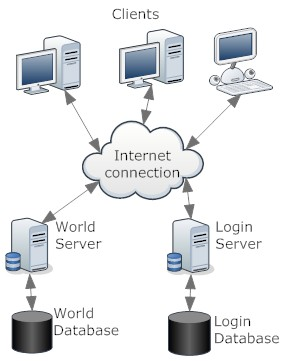
\includegraphics[scale = 0.5]{architecture.jpg}
\caption{Standard MMORPG system architecture}
\label{architecture}
\end{figure}

As can be seen from figure~\ref{architecture}, an MMORPG game has clients that log into the main server by first accessing the login server with their login details. The login server then verifies the login details by sending a query to the login database, and comparing the details. If the username and password are correct, the client gets logged into the world server, where the gameplay takes place~\cite{mmorpgarch}. The client is the software installed on your computer that you use to play the game. It is responsible to take all the input received from the user and the server, and to change the game display accordingly. The data sent and received from the server also has to be encoded and decoded by the client for safety reasons. Most of the data of MMORPG's is stored on your computer, because the Internet is still to slow to send all that data during gameplay. This means that the graphics that make up the game world, all the sounds and even how the monsters look are all stored on your computer in files and databases, and are processed by the client during gameplay.

The server still has a lot of things to compute however, especially considering the amount of players it services. Here is a list of some of the most common computations and functions the server does and sends back to the clients~\cite{serverclient}:

\begin{itemize}
    \item The position of your character in relation to monsters, players and non-playing characters (NPCs)
	\item Whether the monster that the player wants to attack is within range
	\item Whether your player is being attacked
	\item If your attacks are successful
	\item The amount of damage or healing given and received
	\item What loot will drop when a monster is killed
	\item The server also retrieves the skills, spells and items of your character from the database, and regularly saves your data in the database.
\end{itemize}

This type of server-client architecture is common in most of the more popular MMORPGs, and it works efficiently.  %The popularity of some common MMORPGs are shown in Figure \ref{popularity}.
%
%\begin{figure}[htbp]
%\centering
%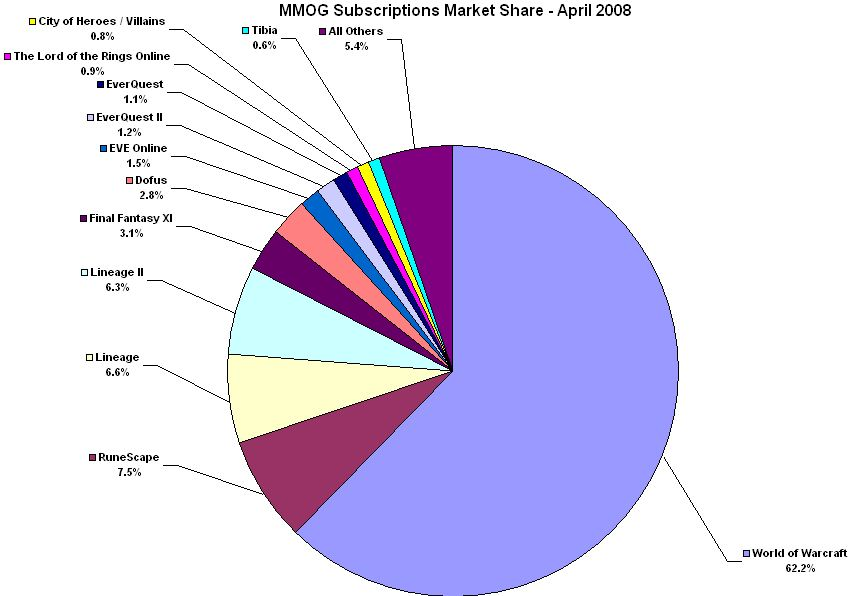
\includegraphics[scale = 0.65]{popularity.jpg}	%http://www.mmogchart.com/Chart7.html how to ref?
%\caption{The popularity of a few MMORPGs measured in percentage of subscribers}
%\label{popularity}
%\end{figure}
WoW is by far the most popular MMORPG in the world, which is why it was chosen for this project~\cite{subscription}.
%As can be seen in figure \ref{popularity}, WoW is by far the most popular MMORPG, which is why it was chosen for this project.


%Explain the basics of MMORPG's and the server-client architecture with the underlying database. Mention that WoW is the most subscribed to MMORPG which is why it was chosen to be the target MMORPG to track players. Mention research done on MMORPGs and why its important. Remember client side states being a security threat mentioned in book on how to exploit.

%\section{A Short History of WoW}

%Give a brief overview of when WoW was created and the previous Warcraft games that inspired it. Mention the expansion packs released, how the client is the same for all subscribers, disregarding whether they have the expansion or not, and also mention how the client is constantly updated, changing key features of how the game works (a few examples could be mentioned). 

%Also talk about where the game might be headed, mentioning growth in the game, how subscribers have now lessened and the possible reasons for it as well as how it will probably become more when new content and expansions are introduced. Remember the plague.

\section{World of Warcaft} %better name?

World of Warcraft is a fantasy role playing game created by Blizzard, set in the fantasy world of Azeroth. Blizzard created the world of Azeroth long before WoW was released, and used it in all of its previous strategy games in the Warcraft series. After Warcraft 3 was released, Blizzard decided to turn the franchise into an MMORPG.

\subsection{Starting the game}
When a user first plays WoW a long process of learning is started since it is a complex game. The first step for a new player is to choose a hero which will be their character or avatar in-game. There are two main sides in WoW, the Alliance and the Horde. Each side has different characters of different races that the user can choose from. These include races such as Humans, Dwarves, Orcs and so forth.
Each race has different classes of characters too, such as a Mage, Priest, Warrior and so forth. The user must create a character by choosing a race, class and name before entering the game world.

%Because there are so many people that play WoW, Blizzard split the game up into different Realms. Each Realm is an exact same copy of the game world, and is only there to split users up into more manageable groups of players. Each Realm has different servers and databases, and characters have to stay in the Realm in which they were created. Realms are also split up into different experience levels. There are different Realms for beginner, moderate and experienced players. 

Once the game is started, there are several non-player characters (NPCs) around, controlled by the server, that gives quests to the local character. Each quest has several rewards for the character, such as experience, items and gold. There are also NPCs that buy and sell items, or repairs items, or teaches your character new skills.

Users interact with the game world by using their keyboard or mouse for movement, and the user interface(UI) to select targets and other objects. %The UI is also useful for providing shortcuts to different spells and other attacks that can be used on monsters in the game.
 Figure~\ref{ui} shows a screenshot where a Warlock is in battle with a monster. The UI can also be seen, with lots of spells being displayed at the bottom of the screen for easy access. The health, mana and names of both the local character and its target is shown in the top left corner of the screen. %Characters consume either mana or rage when using certain abilities, depending on their class.

\begin{figure}[htbp]
\centering
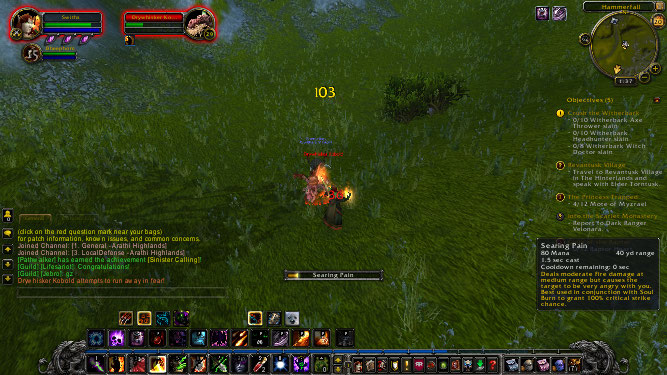
\includegraphics[scale = 0.65]{wowscreen.jpg}	
\caption{A screenshot showing the user interface of WoW}
\label{ui}
\end{figure}

Monsters in WoW are called ``critters'' officially, but are referred to by all the players as ``mobs''. %The mobs in WoW all have a level that indicates how powerful they are. 
%Your character also has a level, and is usually able to kill mobs of the same level and lower easily.
 Killing mobs and completing quests give experience to your character. Your character has an experience bar that measures the amount of experience it has. When this bar is full, the character levels up and the bar is emptied. Each level requires more experience to fill the bar up than the previous level. The top level in WoW is level 85, which can take several weeks of playing to reach.

When a mob is killed, it usually drops items and gold, which is called loot in the game. Items can enhance skills of your character, such as its attack and defense skills. There are many items in WoW, and a lot of motivation to get because they help your character to level up quicker. Items can also be sold for gold, and the gold can be used to buy items from other players or NPCs. 

The game also has professions, which are special skill sets that your character can learn. These include professions such as mining and engineering. Each profession has different advantages to the character, and only two can be learned at a time. 

The game world has large open areas, forests, caves and so forth where mobs are usually found. These are unfriendly areas where your character is in constant danger of being attacked. There are also more friendly areas such as towns where the NPCs that give quests and buy and sell items are found. The largest of these areas are called capital cities, where hundreds of NPCs that teach different skills and sell different things can be found. Capital cities are densely populated and many human players can be found there as they all look for items to buy and so forth.

The most human traffic in a capital city is in its bank and auction house. Players must keep all the items they pick up in their backpack and in satchels. This space is expended quickly when a lot of valuable items are found. The game provides banks in capital cities as extra storage place for players. The most valuable items of a player are stored in banks for future use or to sell them. If a player has a valuable item that is no longer of use to his character, the player can either sell the item to an NPC or at an auction house.

Auction houses list items that players want to sell and for which price. Other players then buy the items that interest them, and the money is transferred to the owner of the item. More gold can be made from selling items in auction houses than from selling them to NPCs. This causes a lot of traffic between auction houses and banks, which are usually located close to each other in capital cities, as players go get their rare items in the bank and then go to the auction house to list them. All this traffic makes capital cities a good place to track player movements to test the software.

All of these different skills, spells, professions and items that belong to your character has to be stored by the server in a database. This data changes frequently during game play and must be sent to and from the database through different queries constantly. It is of interest how much the data of a single player changes during a gaming session, and especially so of multiple players. This will be looked into further in chapter~\ref{database}.

%\subsection{Game Types}
%
%There are a few different game type categories in WoW, each providing a unique gaming experience. The type of player traffic found in each game type is considerably different. The game types where player movement data will be captured as test cases are briefly described here:
%
%\begin{itemize}
%	\item Open-World PvP/PvE
%	
%	This is the first type of gameplay a new player will be subjected to. PvE stands for player versus environment, and PvP for player versus player. The only difference between the two is that in PvP players from different factions can attack each other at any time, while in PvE both players first have to agree to fight before a battle can commence. This gameplay mode is mostly about completing quests, with some mobs being hard enough to require a team of players to defeat. For the most part this game type can be played alone if the user wants to.
%	
%	\item Dungeons
%	
%	The mobs in dungeons are smarter and stronger than the ones that can be found in the open world. A dungeon is a separate instance of WoW that can not be reached by walking around in the game world. A group of five players enter a dungeon together as a team and they work together to defeat the more difficult mobs. These mobs drop rare items and give more experience than normal mobs when killed, providing good motivation for players to enter dungeons.
%	
%%	\item Raids
%%	
%%	Raids are similar to dungeons, but with even stronger mobs which are harder to kill. The areas are bigger than dungeons, and groups of 10 to 25 players usually team up to complete a raid. The most powerful and valuable items can be found in raids.
%%	
%%	\item Battlegrounds
%%	
%%	Battlegrounds are PvP	battlefields , where players of opposite factions are constantly fighting over strategic targets. These include things such as keeping an area under your factions control, capturing the opposing faction flag, or killing the commander of the opposing faction. Some battlegrounds can have hundreds of different players participate in a single battle. Powerful items can also be gained here.
%%	
%%	\item The Arena
%%	
%%	In The Arena, organised teams of 2, 3 or 5 players of opposite factions commence in battle. The objective is to defeat all the members of the opposing faction. Unique items are also found in The Arena.
%	
%\end{itemize}



%
%\subsection{Team Play}
%%The different game types offer lots of motivation for players to team up in WoW.
%Playing a game as part of a team usually has the result that the team works closely together. Since the movement data of players in WoW is of interest, team play is important to keep in mind when tracking player movements.
%There are several different types of teams that can be created in WoW. A user can invite any other player from the same faction  %and in the same Realm 
%to join his group. 
%A group of up to 5 players is called a party, while a group between 10 and 25 players is a raid.
%If you enjoy playing with a certain player, you can add that player to your friend list and be notified when that player comes online, to make playing together again in future easier. 
%
%Another type of group that exists in WoW is called a guild. Parties and raids are only temporary groups, but guilds are permanent groups of players. There are many benefits of joining a guild, such as gaining access to the guild bank and having easier access to other players to form parties or raids.
%
%All of this team play in WoW is one of the reasons that it is thought that players move together often in the game.  % It is especially expected in areas such as battlegrounds and raids. 
%Tracking software can be used to confirm this suspected behaviour and to generate general player movement models. 


\subsection{Factors that influence tracking} 

There are a few factors that need to be kept in consideration when tracking players in WoW. The different levels that players are at give them access to different methods of traveling around. At level 20 a character can learn the skill of Riding, and a mount can be bought. This increases the movement speed of a player with 60 percent. At level 40 the skill can be increased and a faster mount can be bought that increases movement speed up to 100 percent. 

At later levels flying mounts can be bought, and these also get upgraded so that a character of level 85 can have a flying mount that increases movement speed by 392 percent if the proper aura is activated~\cite{mount}.

If tracking data shows what appears to be a player moving through buildings at high speed then it is very likely a player on a flying mount, flying over the buildings. This high movement speed also makes the server send less data to you since it can compute that you will not be able to see the player very long. Figure~\ref{flymount} shows a character on a flying mount, flying over trees into the city of Stormwind.

\begin{figure}[htbp]
\centering
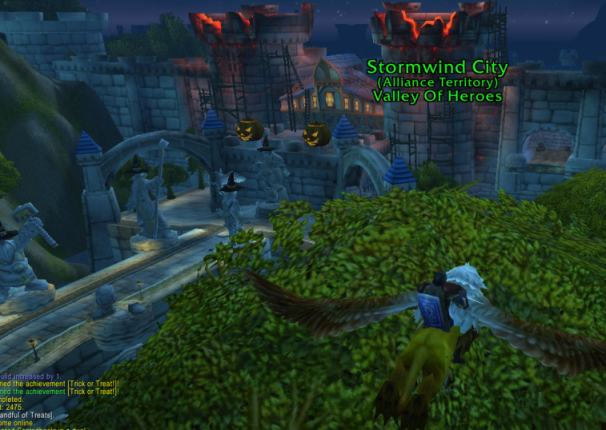
\includegraphics[scale = 0.65]{flystormwind1.png}	
\caption{A player on a flying mount, flying into Stormwind}
\label{flymount}
\end{figure}


The server tries to send your character relevant data and to minimize the irrelevant data. If players are within visual range of your character, but behind a big mountain then it is likely that the server could decide not to send the location of the other player to your client.

When entering WoW, your character suddenly appears in the world without coming from anywhere specific. This could result in tracking data where players appear to come out of nowhere. A player can also log out at any time, which would cause the player to disappear in the tracking data.

Some players in WoW have the ability to cloak themselves, rendering them invisible to other players. The server does not send the location of invisible players to your client, so when a player goes invisible the tracking data will stop without explanation. 

One big problem with tracking players in WoW from South Africa is the Internet. South Africa is behind the rest of the world when it comes to Internet speeds, making latency in the game a frequent phenomenon. A player can appear to be hopping from place to place because of the slow updates received from the server due to the connection. 
All these factors must be considered as a source during analysis if inexplicable location data is found.

 %http://www.wowpedia.org/Mount

%Go into detail about how WoW specifically works, mentioning the different gameplay types, all the skill sets and levelling, battlegrounds, dungeons etc. Mention social parts such as guilds and groups and friend lists. Explain every part that will be mentioned later in thesis as generating a query. Also mention how coordinate system works in game and how mounts and flying mounts work, and how you can log in and out at any time, causing characters to appear and disappear at times. Teleportation and invisibility also needs explaining.

%Could divide this section into further subsections such as the basics, things that generate queries and the more technical parts that users don't have to be aware of such as the coordinate system used. Pictures explaining everything must be included.
\section{ArcEmu}
\label{ch3}

It is of interest to characterise an MMORPG to be able to use this characterisation to drive and test P2P MMORPG systems and to help understand what types of performance are required from an MMORPG to port this to a P2P system. Of particular interest is how an MMORPG handles its data storage especially focusing on how often data is stored and the size of the data stored. A good way to determine this would be to monitor and analyse the data throughput of the database of an MMORPG. Monitoring the database of the official WoW servers would be ideal, but since access to them is prohibited, the database of a private WoW server must be analysed.


ArcEmu is an Open Source, private WoW server emulator. It is compatible with many different operating systems and is compatible with both 32-bit and 64-bit systems. It is developed and maintained by a group of individual programmers for research and recreational purposes, and is written in the C++ programming language. Any interested person can contribute to the project by downloading the code, improving it and resubmitting it.


ArcEmu is not affiliated with Blizzard in any way, and the server is written based on knowledge gained from reverse engineering WoW. ArcEmu can be downloaded for free and used to host your own private WoW server. It currently only supports the WoW client up to version 3.5.5a and attempting to connect to an ArcEmu server with an updated WoW client will therefor not work. The client first needs to be downgraded to be compatible.


ArcEmu is run on your personal computer (PC) and can provide access to users in three different ways:

\begin{enumerate}
	\item From your local PC. 
	This means that the server and the WoW client are run on the same machine.
	\item From the local network.
	With this setup users can connect from any other PC connected to the same network as the PC that the server is run on.
	\item From the Internet.
	With this setup, any user that has an Internet connection can access the server via that connection.
\end{enumerate}

The first setup is used in this project. 

ArcEmu provides only the code needed for the core of the server. The NPCs and quests that populate the world are all stored in databases that can be downloaded from other open source projects. The maps and other required data are also not provided, and need to be extracted from the WoW client.

There are many guides available online on how to properly install and configure ArcEmu, and the details will not be discussed in this report~\cite{arcemu}.

For ArcEmu to work properly, a compatible database is required. The database part of the server is a combination of the database framework needed and the actual data stored in the databases.
The only database framework supported by ArcEmu is MySQL which is discussed in more detail in chapter~\ref{database}.

ArcEmu uses three databases to store the different data sets needed to run the game. The first one is the logon database which contains the account information of users. The second one is the character database. This database stores all the different values of your character, such as how many items, spells, skills and gold it has. The last database is the world database. All the data about NPCs, quests, items and so forth are saved in this database. Figure~\ref{arcdata} shows how the different parts of these programs communicate with each other.

\begin{figure}[htbp]
\centering
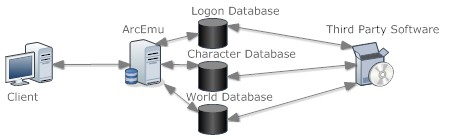
\includegraphics[scale = 0.65]{arcemu.jpg}	
\caption{The architecture used by ArcEmu and how its databases can be accessed}
\label{arcdata}
\end{figure}


Once ArcEmu is set up properly, the client can connect to it as if it were the real WoW server. All the data about NPCs, quests, items and so forth is sent to the client by the ArcEmu server. The server also receives data from the client about what actions the character is doing, which is then distributed to any other connected clients. Communication to and from the database is done exclusively by the server, but it is triggered by actions that the client does. Since ArcEmu uses MySQL, the database can be fully accessed without the use of the server. Figure~\ref{arcdata} shows how third party software has access to the databases used by ArcEmu.

Using ArcEmu thus grants full access to the database of an MMORPG, which can then be monitored and analysed to create models of how MMORPGs store and retrieve data. How exactly this is done is discussed in further detail in chapter~\ref{database}.
%\chapter{ArcEmu} %better name?
\label{ch3}

This chapter provides a brief description of what ArcEmu is, and how to get it working properly.

\section{Description}
In order to better understand how the database of WoW works on the server side, a private server is needed for analysis purposes. If a private server is set up, the database can be accessed and analysed to discover how much traffic is created to and from it by players connecting to the game. The most frequent queries can be discovered as well as the inter arrival time of the different queries, which would be useful in creating a model of traffic generated to the database of a MMORPG.

ArcEmu is an Open Source World of Warcraft server emulator. It is compatible with many different operating systems and is compatible with both 32-bit and 64-bit systems. It is developed and maintained by a group of individual programmers for research and recreational purposes, and is written in the C++ programming language. Any interested person can contribute to the project by downloading the code, improving it and resubmitting it. 
%http://arcemu.org/forums/index.php?showtopic=16520
ArcEmu is not affiliated with Blizzard in any way, and the server is written based on knowledge gained from reverse engineering WoW. ArcEmu can be downloaded for free and used to host your own private WoW server. It currently supports the WoW client up to version 3.5.5a and attempting to connect to an ArcEmu server with an updated WoW client will not work. The client first needs to be downgraded to be compatible.

Programmers constantly update ArcEmu and provide a short description of what functionality is added to the server with the update. It is often updated several times a day, so it is better for users to read the description of the update and decide if its worth the effort of updating for the changes introduced.

ArcEmu is run on your personal computer (PC) and can provide access to users in three different ways:

\begin{enumerate}
	\item From your local PC. 
	This means that the server and the WoW client are run on the same machine.
	\item From the local network.
	With this setup users can connect from any other PC connected to the same network as the PC that the server is run on.
	\item From the Internet.
	With this setup, any user that has an Internet connection can access the server via that connection.
\end{enumerate}

The first setup is used in this project. 

ArcEmu provides only the code needed for the core of the server. The NPCs and quests that populate the world are all stored in databases, that can be downloaded from other open source projects. The maps and other required data are also not provided, and need to be extracted from the WoW client.  Section \ref{setup} briefly discusses what is required to get a working ArcEmu server.

%Discuss when ArcEmu started and how it still progresses. Mention other private open source servers available. Talk about the fact that all private servers that are open source work with an older version of the client, making it incompatible with the current client.


\section{Setup} %better name?
\label{setup}
The process for setting up ArcEmu depends somewhat on the operating system used. The method described here is specifically for Windows devices.
There are many guides available online on what steps need to be followed to setup ArcEmu, so the discussion here will be very high level and only for the purpose of understanding what different parts of software make up the ArcEmu server.

The first step is to download and compile the source code of ArcEmu. %The source code is downloaded using Subversion client software and the code is then compiled using the CMake build system.
The successfully compiled code is called the core of the server. It is still completely unusable without map files from the WoW client and a database, and a tool to extract these are included in the core.

For ArcEmu to work it requires maps, vmaps and DBC files from WoW. The extraction tool included in the core is called ad.exe and must be copied to the WoW folder and executed. It will take a few minutes to successfully extract all the needed files. When it is done, the files need to be copied to the ArcEmu folder.

The next step in the setup is getting a database that works with ArcEmu. The database part of the server is a combination of the database framework needed and the actual data stored in the databases.
The only database framework supported by ArcEmu is MySQL which is discussed in more detail in chapter \ref{database}. Getting the data that is required to be in the databases is what is important for the setting up process.

ArcEmu uses three databases to store the different data sets needed to run the game. The first one is the logon database which contains the account information of users. The second one is the character database. This database stores all the different values of your character, such as how many items, spells, skills and gold it has. The last database is the world database. All the data about NPCs, quests, items and so forth are saved in this database.

The user must choose one of several similar Open Source projects that create these databases. These databases are classified as Blizzlike if they strive to make the data contained in them similar to the official WoW game. For this project the Blizzlike database called WhyDB was used. 

Since the databases are from a separate project, a method is needed to make sure that the structure ArcEmu expects is compatible with the database. To do this, queries are created by ArcEmu that must be run after the databases are installed which makes the structure compatible. 

After the database is installed, the configuration files of ArcEmu needs to be changed to fit your unique setup.
%The databases and the queries generated for them by ArcEmu is discussed in chapter 4.
After ArcEmu is successfully set up, the server needs to be started and then clients can start connecting to it. Each query that is generated to the databases from the server can then be analysed in further detail to determine the type of database traffic generated in MMORPG games. This is discussed further in chapter \ref{database}.

%Explain how to set up ArcEmu briefly. Talk about how MySQL is used to store the world, character and logon databases, and how to load them. Explain the different online databases available etc.

%Show proof that ArcEmu was set up correctly and is in working order.




\chapter{Database Analysis}
\label{database}
In chapter~\ref{ch3}, the WoW private server, ArcEmu, was discussed. In this chapter the underlying database used by ArcEmu is discussed, as well as methods and commercial software available to analyse the amount of queries made to the database as well as its data throughput. This data needs to be captured and analyse in order to characterise the data storage methods used by a mature MMORPG. The data will then be used to try to replicate the same type of performance on a P2P MMOG system. 
A strategy is developed in this chapter that will be used to find out which actions in WoW cause which queries to be generated by the server.

%WoW client software is set up to connect with ArcEmu to determine what kind of queries different in-game actions generate. These results are then used to determine which test need to be done on the database in chapter~\ref{results}. %Different tests are then run with the ArcEmu setup to determine how the database responds to a larger amount of clients connected to the same database.

\section{MySQL Explained}
%http://dev.mysql.com/doc/refman/5.6/en/history.html
MySQL, pronounced ``My Ess Que Ell'', is the most popular Open Source Structured Query Language (SQL) database in the world~\cite{mysqlhist}. It is named after the daughter of co-founder Monty Widenius, My. 

After a fresh installation of MySQL 5.5, a graphical user interface (GUI) is provided to set up the MySQL server for the first time. Once the server is set up however, all interfaces with the MySQL database is text based through the command line. There are several free programs available that provides a GUI to create, edit and view tables and databases on the MySQL server. Navicat is one of the more popular such programs, and was used to set up ArcEmu and view the tables in the databases throughout this project.

%Every time the server of MySQL is started it reads the start-up settings from configuration files stored on the computer. This means that even if the configuration of the server is changed while it is running through the command line, the changes will only last until the server is restarted, when the default configuration in the configuration files will be restored. 
There are only two ways available to study the queries that are made to a MySQL database, and that is by activating the general log, or the slow query log, or both.

\subsection{MySQL Logs}
%It is important to activate the general and slow query logs by typing the proper commands in the configuration file if it is required that the logs are always active. This is done by finding the configuration file (called my.ini in version 5.5) in the installation directory and typing in the commands shown under [mysqld] in figure \ref{mysqlcom}.
%
%\begin{figure}[htbp]
%\centering
%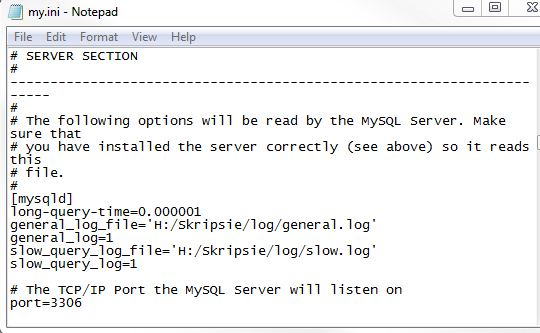
\includegraphics[scale = 0.65]{mysqlcom.jpg}	%http://www.mmogchart.com/Chart7.html how to ref?
%\caption{The configuration file of MySQL with logs enabled}
%\label{mysqlcom}
%\end{figure} %haal die dalk uit?

Enabling the general log in MySQL makes the server log each query that is made to the server from clients. This includes the type of query, the specific table it was made on and the time it was made. The response from the server is not logged at all however, which means that the general log does not provide any information on the amount of data that was sent back from the server or the time it took for each query to be sent. The general log is thus only useful to get an idea of how many queries are made to the database, and which queries occur the most.

Enabling the slow query log gives the user access to a little bit more information, but at a cost. It can slow down the response of the database under heavy load, but this was fortunately not a problem for the tests done on it. Another setback of the slow query log is that it only logs queries that take longer than a set amount of time. That value was set to 0.000001 seconds in the configuration file, which is its smallest possible value. The value is small enough that most queries made are logged, but some small queries happen faster than 0.000001 seconds and are then omitted from the logs. 

The following data is logged by the slow query log:

\begin{itemize}
	\item The time the query was made, rounded to the nearest second.
	\item The type of query made, the table it was made on and the user who made it.
	\item The amount of rows that were examined to make the query.
	\item The amount of rows that were sent back by the server as a result of the query.
	\item The time it took the server to find the right results of the query.
	\item The time it took the query to be completed.
\end{itemize}

With all of this data, a thorough analysis of the queries made to the database can be made and the average amount of queries made over time by players can be concluded with test data. The most frequent queries can also be determined as well as the time interval in between each query.

%Explain how MySQL works, how to access the tables contained in the database, how to make queries.
%Explain which logs are supported, how they work and how to enable them. Discuss the data that can be extracted from the logs and how they can be parsed by either your own program or using commercial software available for that purpose.


\section{MONyog} %prente maybe?

The usual text based command line interface of a MySQL server makes it difficult to use some of its features, and makes analysis of the databases it contains harder too. For this reason there exist many third-party applications that provide a more user-friendly GUI to use and analyse databases on a MySQL server. 

The data contained within the two logs that the MySQL server creates can be extracted by writing a parser program that takes a log file as input and parses the information it contains to calculate statistical data for the database. The amount of queries created over a certain amount of time, and the amount of times each query is made and so forth can be extracted in this way. There already exist third-party applications that provide this functionality however. MONyog is one of those applications,  and it was used to analyse the queries made to the ArcEmu MySQL databases.

MONyog sends status queries to the MySQL server every 5 minutes to get data on how the server performs throughout the day. This provides additional information about the database which can then be retrieved and analysed for the times that the WoW client was connected to the server.

MONyog also has the ability to parse both the general and the slow query log, to extract more information from them, which is displayed  in tabular format. All these analysis tools will be used to analyse how the database of the private WoW server responds to clients playing the game on it. Figure~\ref{monyog} shows the GUI provided by MONyog to analyse MySQL databases, with the current window showing the total size that the data of all the databases are taking up on the disk in megabytes. 


\begin{figure}[htbp]
\centering
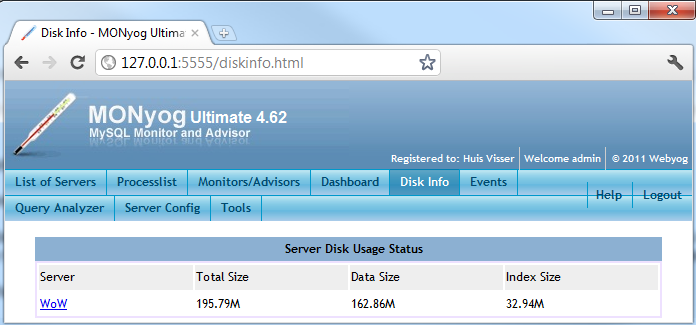
\includegraphics[scale = 0.65]{monyog.png}	
\caption{MONyog GUI showing the total size of the data contained in all the MySQL databases}
\label{monyog}
\end{figure}


%Briefly describe what MONyog is and how it works. Discuss how it enables users to analyse database data throughput and queries made to the database. Explain how the program was tested for accuracy and integrity of information, and show proof with images. Compare results found in logs to the output generated by monyog parser.


\section{Database Analysing Strategy}
\label{datastrategy}

With all the tools needed to analyse the databases and tables in place, a strategy is required on how to start characterising the data storage methods used by an MMORPG. A method is needed on how to determine when, why and how many queries are made to the database by the server. The nature and size of the queries are also of interest. 

From installing the databases it is known that the following data are contained in them:

\begin{itemize}
	\item The account information of all the users.
	\item The items, spells, skills, location and other data of every character that has been created.
	\item The NPCs, and quests they give and items they sell.
	\item All the mobs and where they are located and which loot the drop.
\end{itemize}


This data can give a general idea of what data needs to be saved and retrieved by the server, and what could be a trigger that causes the server to generate a query to the database. The account information would be needed to be compared to the data that users type in when they log into the server. It is probable that the server makes a query to the database to retrieve this information either in batch when the server is started, or every time a new user logs into the game.

When a user is logged in, the game goes to the character choosing or creating screen, where the user can either choose a character to log into the world with, or create a new character and then log into the world. For either of these options information about what skills and so forth the character will have is required, and it is probable that a query will be generated to the database every time a user creates a new character or chooses a character to play with.

When the user enters the world, the NPCs and the quests they give, as well as all the mobs, is already there. They continue to exist in the game world when the user logs out since other users might still be in the world. It is thus expected that all of this data is retrieved from the databases before any characters log in, as the server is started.

As the user is playing, the character will start quests, level up, gain skills and so forth. Many of these actions will change the properties of the user and this information needs to be saved in case the user logs out, so that it can be retrieved when the user decides to play again. It is therefore suspected that the following actions, among others, of any character will generate queries to the database:

\begin{itemize}
	\item Starting a quest.
	\item Completing a quest.
	\item Gaining any skill.
	\item Learning a new spell.
	\item Learning a new profession.
	\item Killing a mob.
	\item Picking up loot.
	\item Buying and selling items.
\end{itemize}

Whenever a player dies the character is turned into a ghost and teleported to the nearest graveyard. Information about where the nearest graveyard is or how the ghost must look would be needed, which suggests that another query would be made to the database by the server whenever a character dies. This could generate yet another query when the player finds its body and is reincarnated. 

After playing the game for a while, the user will log out of the world, and the server does not need to update other clients about the position of the user anymore. Any final data, such as the current position of the player and the current spells active and so forth also need to be saved. Queries would thus be generated whenever a character logs out of the game.


With a good idea of what actions in WoW will generate queries, a method is needed to test this expected behaviour. The general and slow query log will have a record of every query made, so a player could play the game and perform all of these actions and compare the logs with the time the actions were performed in the game. It would be better to isolate the data to get more precise results however. The following strategy will be followed in order to test whether the server behaves as expected:

The general and slow query logs will be activated and a user will log into the game. The logs will then be copied, saved and cleared before anything else is done in the game. After the logs are cleared, the user will choose a character to enter the game world, after which the logs will again be copied, saved and cleared. The user will then perform all the actions in the game that is suspected to generate queries, saving and clearing the logs after each action and labelling each log with the action it represents. Finally the user will log out and save the last logs. This should generate compelling data to analyse the behaviour of the server through every action that characters perform when playing the game.

After doing these tests and analysing them, a good picture can be formed on when and why the server stores and retrieves data. More data will still be needed to analyse whether this behaviour is consistent when a player plays the game for a long time, and even more importantly, when more than one player is playing at the same time. To determine this, more tests are needed.


\subsection{Further Tests} %better name?
\label{further}

All the data that will be collected up till now will be very fractioned and only relevant to one specific action. To gain information about the behaviour of the server in general, the logs will once again be enabled and a user will log in and play the game normally for three hours. It is of interest to determine how much queries are generated by a player in a typical gaming session, what the most frequent queries are, and the inter-arrival time of the queries in general. 

Of further interest is how the server responds when more than one player is logged in simultaneously and playing the game. To simulate more players on the server, a program called a bot (short for robot) is used. This program is able to control a WoW character and play the game to a certain extent. It follows a path that has been set out for it specifically, and attacks, kills and loots mobs on that pathway. Quests need to be started and completed manually however, and the behaviour of the character is not the same as that of a human player, but its the closest that can be simulated.

Up to four characters can be logged onto the same server by using this software. These test will be done and further discussed in chapter~\ref{results}, where the results of the tests will also be analysed.

%Now that it is known which actions in the game cause which queries, tests need to be done to determine how much queries are generated by a player playing the game normally for a gaming session. It is also of interest if the queries multiply with the amount of players when more players are playing the game. The most frequent queries and their inter-arrival time is also of interest to be able to create a model of normal database behaviour.
%
%To simulate more players on the server, a program called a bot (short for robot) is used. This program is able to control a WoW character and play the game to a certain extent. It follows a path that has been set out for it specifically, and attacks, kills and loots mobs on that pathway. Quests need to be started and completed manually however, and the behaviour of the character is not the same as that of a human player, but its the closest that can be simulated.
%
%Up to four characters can be logged onto the same server by using this software. These test will be done and further discussed in chapter \ref{results}, where the results will be of the tests will also be analysed.

%With the tools needed to analyse the databases and tables in place, more information is needed on which actions of the character causes which queries to be generated. To gather this information the general and slow query logs are needed. Before starting with this exercise a list of actions done by the character that is expected to change some game-state which would generate a query of some sort is made. This includes things such as killing mobs, taking loot, logging in, doing and finishing quests, gaining skills and leveling up, to  name a few. 
%
%At first the logs were cleared completely. After that a certain action was performed in the game and the logs were copied and saved after performing the action. The logs were then cleared once again before the next action was performed and so forth. With this method, several actions and their associated queries were saved for further analysis. 
%
%What was surprising was that the following behaviour from the database was found: most of the actions performed by the character did not generate immediate queries. The expected queries did however happen  a few seconds or even minutes after the action was performed. This suggests that the server saves all actions that will generate queries in variables at first. A queue of queries is then created that is executed either when the queue gets too full or after a certain interval. There are however certain actions that always generated immediate queries. This could mean that those queries are either big enough for the queue of queries to be considered full enough to be executed, or they are simply of higher priority and thus handled immediately. When any query is executed however, the queue is emptied and all the queries that did not take place immediately is executed along with the others.
%
%This behaviour from the server makes sense upon reflecting on it, since it would concentrate queries made to the database when a small amount of queries need to be made. Extensive testing was done to test this expected server behaviour, but after generating as much queries as possible with five clients logged in simultaneously, the queries still only happened after a counter of sorts triggered the queries to be made. This suggests that the server has a timer that generates an interrupt of sorts after a set amount of time has passed. This interrupt then causes the server to make all the queries that are needed to the database. This is the equivalent of saving all the changes that have happened in the meantime.
%
%It is sensible for the server to behave in this way, because the server has a lot of other things that it is responsible for, such as generating all the actions of the mobs and sending location information to all the clients and so forth. If every action that caused a change in game state generated an immediate query then the server would constantly be busy sending information to the database, causing lag in its normal and more important function of communicating with the client. This behaviour would become worse when more clients connect to the server, and the game would soon become unplayable. 
%
%The following pattern was discovered by analysing hundreds of queries made to the database to ensure its legitimacy: there are two counters that generate queries constantly looping on the server side. The one counter generates a query to check if any of the players has sent mail to any of the other players every three minutes. This is the shorter of the two counters, which is understandable because other players could be waiting for the mail to be sent, which makes it a higher priority query.
%
%The other counter generates a ``START TRANSACTION'' query every five minutes. This query starts a sequence of queries that save all the changes to all the characters that have happened in the past five minutes. This includes all new skills and spells learned, gold collected, quests accepted and completed and so forth. 
%
%Table \ref{queries} lists all the actions that were found to generate queries immediately, as well as the amount of queries that they generate. The queries generated by starting the ArcEmu server are also listed. Starting ArcEmu generates the largest amount of queries by far, but this should only happen once per week at a maximum, when servers are restarted for maintenance purposes.
%
%
%\begin{table}[htbp]
%  \centering
%  \caption{List of actions in WoW that generate immediate queries}
%    \begin{tabular}{lrlr}
%    \addlinespace
%    \toprule
%    \textbf{Action in game} & \textbf{} & \textbf{Queries} & \textbf{Total time to execute} \\
%    \midrule
%    Starting ArcEmu &       & 1845 queries & 27.199 sec \\
%    \midrule
%    Logging in &       & 3 queries & 1.047 sec \\
%    \midrule
%    Creating a character &       & 18 queries & 0.765 sec \\
%    \midrule
%    Entering World &       & 23 queries & 0.597 sec \\
%    \midrule
%    Selling Items &       & 1  query & 0.056 sec \\
%          &       & per item &  \\
%    \midrule
%    Dying &       & 2 queries & 0.059 sec \\
%    \midrule
%    Resurrecting &       & 1  query & 0.049 sec \\
%    \midrule
%    Logging Out &       & 76 queries & 0.078 sec \\
%    \bottomrule
%    \end{tabular}%
%  \label{queries}%
%\end{table}%
%
%
%All of these actions in WoW are of high priority, which is why the server deems them important enough to break its usual cycle of only saving changes to the database every few minutes. Most of these actions only happen once per gaming session however, so they should not have a large effect on the performance of the server.
%
%The actions in the game that happen most frequently, like gaining skill points, levelling up and starting and completing quests are all processed at the same time, and only add one query per action to the list. Attributes like which spells a character knows and which items are in their backpacks are all both deleted and inserted into the database every five minutes with the START TRANSACTION query that happens. This will happen even if the character does nothing in that time. Analysing several logs revealed that the START TRANSACTION query generates approximately 65 queries for every player every 5 minutes when the player does nothing.

%Discuss how the game was played for hours to generate queries, explain what was done in game and which corresponding queries were created for each action. Mention resulting queries from playing for 3 hours and how database reacted etc.


%\section{Database Tests} %better name?
%Now that it is known which actions in the game cause which queries, tests need to be done to determine how much queries are generated by a player playing the game normally for a gaming session. It is also of interest if the queries multiply with the amount of players when more players are playing the game. The most frequent queries and their inter-arrival time is also of interest to be able to create a model of normal database behaviour.
%
%To simulate more players on the server, a program called a bot (short for robot) is used. This program is able to control a WoW character and play the game to a certain extent. It follows a path that has been set out for it specifically, and attacks, kills and loots mobs on that pathway. Quests need to be started and completed manually however, and the behaviour of the character is not the same as that of a human player, but its the closest that can be simulated.
%
%Up to four characters can be logged onto the same server by using this software. These test will be done and further discussed in chapter \ref{results}, where the results will be of the tests will also be analysed. %This was done and the reaction of the database was compared to the data captured with only one human player playing the game. These results are analysed and compared in chapter \ref{results}.

%Not sure if this belongs here? Mention resulting queries from playing for 3 hours and how database reacted etc. and how bots were added. Explain results expected from adding bots, show results from adding them and explain differences.
%Will have to be careful to not go into too much detail since this needs to be discussed in a separate chapter in more detail. Perhaps only mention that the tests were done here and leave the results for later?




%\begin{table}[htbp]
%  \centering
%  \caption{List of actions in WoW that generate immediate queries}
%    \begin{tabular}{lrlr}
%    \addlinespace
%    \toprule
%    \textbf{Action in game} & \textbf{} & \textbf{Queries} & \textbf{Total time to execute} \\
%    \midrule
%    Starting ArcEmu &       & 2 UPDATE queries & 27.199 sec \\
%          &       & 2 INSERT queries &  \\
%          &       & 3 DELETE queries &  \\
%          &       & 13 Connect queries &  \\
%          &       & 1825 SELECT queries &  \\
%    \midrule
%    Logging in &       & 1 UPDATE query & 1.047 sec \\
%          &       & 2 SELECT queries &  \\
%    \midrule
%    Creating a character &       & 5 SELECT queries & 0.765 sec \\
%          &       & 13 DELETE queries &  \\
%    \midrule
%    Entering World &       & 1 UPDATE query & 0.597 sec \\
%          &       & 1 DELETE query &  \\
%          &       & 2 INSERT queries &  \\
%          &       & 19 SELECT queries &  \\
%    \midrule
%    Selling Items &       & 1 DELETE query & 0.056 sec \\
%          &       & per item &  \\
%    \midrule
%    Dying &       & 1 DELETE query & 0.059 sec \\
%          &       & 1 INSERT query &  \\
%    \midrule
%    Resurrecting &       & 1 DELETE query & 0.049 sec \\
%    \midrule
%    Logging Out &       & 1 COMMIT query & 0.078 sec \\
%          &       & 4 SELECT queries &  \\
%          &       & 20 DELETE queries &  \\
%          &       & 51 INSERT queries &  \\
%    \bottomrule
%    \end{tabular}%
%  \label{queries}%
%\end{table}%
\chapter{Player Tracking}
\label{ch5}

In chapter~\ref{database}, a strategy was developed to determine which actions in the game cause which queries to the database. Further required tests were also discussed. 
In this chapter we look at methods available to gather player location data from the game. A specific method will then be chosen and every detail will be discussed and tested thoroughly. Other functions of player tracking software such as logging the location data, graphically displaying it and reading the logs will also be discussed in detail. 

\section{Different Methods}
This section discusses the different methods available to get the location data from players in WoW. The methods are then compared to each other to determine the best one to use.

\subsection{Server Side Tracking}
There are a few open source private WoW servers available online, such as ArcEmu, mentioned in chapter~\ref{ch3}. The server calculates the movement of all the NPCs and mobs in the game, and it receives all the locations from all the different clients too, which it sends back to all the clients for them to display. Since the private server is Open Source, the source code can be studied to determine where in the program the packets are handled. Extra code can then be added to the server to log all the location data for analysis purposes. 

%This method was disregarded without much consideration however, since the players need to be tracked on live servers, where server side access is not a possibility. Methods that are done on the client side are thus the only viable options.

\subsection{Intercepting Packets}
The client constantly sends updates of your current location to the server so that the server knows where you are in the game world. The locations of all the other players, NPCs and mobs that are in close proximity to your avatar (this is a radius of about 230 meters in-game) are also constantly sent to your client by the server. Before the client or server sends this information, it is encrypted. This is illustrated in figure~\ref{encryption}.

\begin{figure}[htbp]
\centering
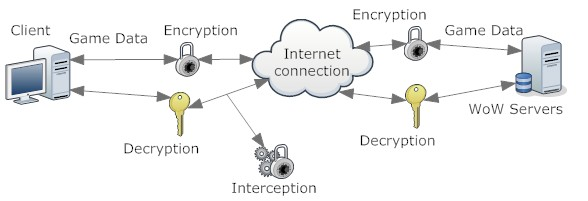
\includegraphics[scale = 0.6]{encrypt.jpg}	
\caption{WoW Server-Client Communication}
\label{encryption}
\end{figure}

The encryption and decryption is done in the client, so all intercepted packets will still be encrypted. WoW used XOR encryption on its header files since its release up until version 3.0.9. This encryption is not very secure and was easy to decrypt~\cite{xor}. The method of intercepting packets was done by~\citet{previous} to do their study on player movements in battlegrounds. 

WoW changed the form of encryption used with the release of patch 3.1.0 to RC4, which is a more secure form of encryption~\cite{rc4}. It is still possible to decrypt packets that are encrypted with RC4, but the key first needs to be found in memory. %Fortunately there are other methods available which also make use of memory reading that are much simpler, which is why this method was discarded.

\subsection{Reading Decrypted Packets}
When the client has decrypted the packets, they are moved to a set place in the clients memory where the client has to decide what the decrypted packets mean and what to do with them. By reverse engineering the WoW.exe file, this specific location in memory can be located and the decrypted packets can be read from the client's memory. This method is very viable, but a lot of the packets that are received will contain irrelevant information. The program will need to inspect every received packet and filter out the relevant ones for further analysis. %This method was discarded because there is a simpler and more efficient method available, discussed next.
Figure \ref{methods} shows visually where the decrypted packets are located that can be read.

\begin{figure}[htbp]
\centering
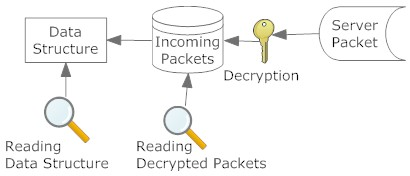
\includegraphics[scale = 0.65]{methods.jpg}	
\caption{Two methods of getting player location data}
\label{methods}
\end{figure}

\subsection{Reading WoW Data Structure}
The decrypted packets are all read by the WoW client to determine what they are for. When the client knows what a packet is for, it sends the packet on to where ever its right place in memory is. This process sorts all the received data into its right place in the WoW data structure. By reverse engineering the client, the data structures can be deciphered as well as the memory locations of the sorted data. All the data about players, NPCs and objects within visual range of your character in the game is sent to your client. That data is stored in memory, and can be read with the knowledge gained from reverse engineering the client. The data can then be displayed or stored after reading it. Figure~\ref{methods} shows where the data structure can be read from packets the server sends.

\subsection{Comparison}
The point of all these different methods of gaining the location of players is to be able to save and analyse the data to create movement models based on the movement of real people. The only place to gain meaningful movement data from WoW is by logging the movement of players on the live servers provided by Blizzard. 
The first method described requires access to the source code of the server to work. This method can thus be disregarded from the start, since access to the server is blocked. Only client-side tracking is considered viable.

The remaining three methods all require a program to read information from the client's memory. Intercepting the packets while they are still encrypted creates a lot of unnecessary effort if the memory is going to be read anyway. The second method of reading all received packets from memory gives exactly the same data as the first method of decrypting all received packets, but without the need to decrypt anything. Reading the received packets from memory is thus a better option than intercepting the encrypted packets. 

The method of reading the data structures of WoW from the client memory gives direct access to relevant data. Knowledge of the data structure used by WoW allows you to read the location data of players directly where it is stored. This method is better than reading all of the packets, where a lot of irrelevant data has to be sorted through. The method of reading the data structure is considered to be the best option available and is the method that will be used in this project.

%gaan soek wanneer encryption verander het. add references vir feite

%Discuss the different methods available, and briefly mention their complexities and difficulty. Motivate why you chose the method you chose.

\section{WoW Internal Data Structure}
Most programs use data structures to work with the variables needed to perform their different tasks. These include arrays, trees, structs, linked lists and so forth. With proper knowledge of how a program's data structures work, other programs can gain access to its data and functions by reading from and writing to the proper places in memory. When the source code of a program of interest is hidden, programmers use programs called disassemblers to gain information about the data structures of the program of interest. This is a complex and time consuming task, especially when there is a lack of previous knowledge of the program being disassembled. 

WoW is a very popular game however, and the gaming community has studied its data structures in fine detail. There is thus a lot of information available online on how to look for the right addresses to WoW's data structures, their respective sizes and how they link together. %The procedure to follow to find one address will be briefly discussed ~\cite{idapro}.
There are also many tutorials available online that show you how to reverse engineer WoW to gather this information~\cite{idapro}, but that is outside the scope of this project. Fortunately all the necessary information is usually posted on public forums such as www.ownedcore.com on the same day that a new patch is released.

\subsection{ASLR} %die subsection is dalk nie nodig nie?

Up until version 3.x of WoW, the base address of the process was always located at address 0x401000 in memory~\cite{wowbase}. This allowed programmers to use absolute addresses to all the data structures they wanted to access. The developers of WoW changed this from version 4.x onwards by adding support for address space layout randomisation (ASLR), to make WoW more secure. 

ASLR is security technology that makes a system more secure by making it harder for attackers to exploit existing vulnerabilities in the system. This is accomplished by randomising the memory layout of an executing program, which means that where an attacker could previously know exactly where a function would be in memory, the attacker would now have to guess the location in memory. This significantly decreases the chances of a single exploitation attempt being successful. It can also cause the program to crash, which limits the amount of exploitation attempts the attacker can practically make. ASLR is integrated into several operating systems, and is enabled by default in Windows Vista and Windows~7~\cite{aslr}. 
%soek references!

%gan maybe meer in detail in oor ASLR later?

%To decompile an executable file, the first thing you need is decompiler software. For this example, IDA Pro Disassembler will be used. The steps needed next are listed below:

%\begin{enumerate}
%	\item Open IDA Pro with administrator rights, and load the WoW.exe file into the program by clicking on File and Open.
%	\item A popup window should display after clicking open, where you should select the Portable Executable (PE) option.
%	\item After IDA has disassembled the binary it will show you a view of some subroutines and their addresses, which is not of much help. The best place to start looking is in the ``Strings Window''. To access this window, press ``Shift + F12''. This window will be used to search for something familiar.
%	\item Press ``Alt + T'' to search for a specific string, for this example search ``GetMinimapZoneText''. The program should now resemble Figure \ref{idascreen}.
	
%	\begin{figure}[htbp]
%\centering
%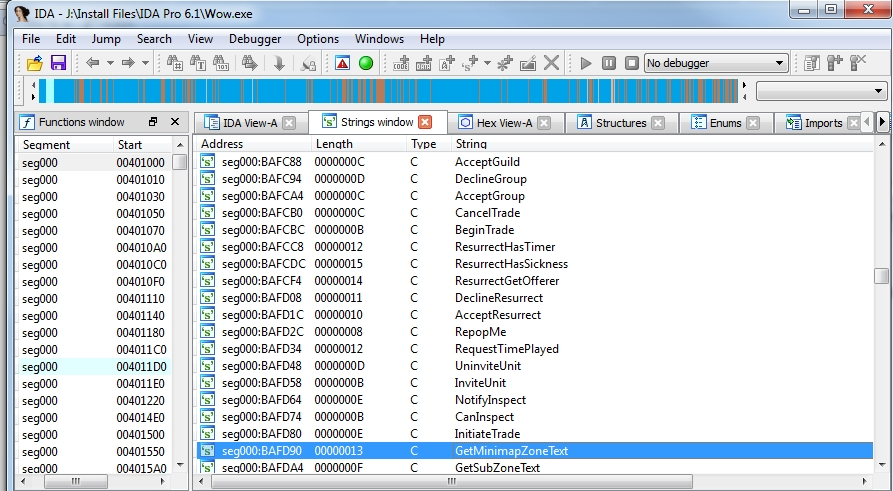
\includegraphics[scale = 0.6]{disassembled.jpg}	
%\caption{Typical Strings Window in IDA Pro}
%\label{idascreen}
%\end{figure}
	
%	\item Double clicking the ``GetMinimapZoneText'' line in the program will show you the ``IDA View-A'' of the code.
	
%\end{enumerate}

\subsection{Data Structures}

Extensive research has been done by the gaming community on exactly how the data structures of WoW works. The data structure of WoW is large and has information about everything that appears in the game. An overview of the complete data structure of WoW would contain a lot of data that is irrelevant to this project, therefore a simplified version that only includes relevant data will be provided here. All this information is the result of the hard work by people who reverse engineered WoW, and the validity of the data was confirmed by research done in the Memory Editing section of the OwnedCore forums~\cite{objman} and through thorough testing of the code.

The starting point and entry into the WoW data structure is the base address. This address can be found by searching for the base address of the process called wow.exe during runtime, which is the easiest way to circumvent ASLR. The WoW community have come up with a set of names for certain parts of the data structures to make sharing the offsets to those structures easier and more readable for everyone. The data structures are all tied together by offsets added together to create pointers to the actual data. This can become complex, with pointers pointing to pointers that finally point to the data that is needed.

Using the base address of the WoW process as starting point, access to some data can be gained by adding offsets to the base address and then reading that address. Here is a list of relevant information that can be gained directly by adding offsets to the base address of WoW and then reading that address:

\begin{enumerate}
	\item The name of your current player.%Base + playerName = Current Player Name. This address must be read as a string.
	\item The globally unique identifier(GUID) of your currently selected target in the game.%Base + LastTargetGUID = Globally unique identifier of your current target in the game. This must be read as an unsigned 64-bit integer and will return zero if no target is selected.
	\item An offset needed to access the object manager. This offset is called the client connection offset.%Base + clientConnection = ClientCon (address that needs to be added to another address to access the object manager). This must be read as an unsigned integer.
\end{enumerate}


There is a data structure in the WoW process that is referred to by the WoW community as the object manager. This data structure can be traversed similarly to a linked list once access to it has been gained, and it holds a list of all the WoW objects that are in close proximity to your character. It also stores many details about each object such as its name, type and location in X, Y and Z coordinates. Access to this data structure is thus exactly what is needed to extract the location data of all the players in close proximity to your character. 

\begin{figure}[htbp]  %maybe move figure to earlier in text.
\centering
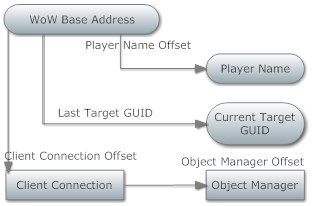
\includegraphics[scale = 0.65]{objmanonly.jpg}	
\caption{How to access the object manager}
\label{datastruct}
\end{figure}


As can be seen simplified in figure~\ref{datastruct}, access to the object manager can be gained by adding the client connection offset to the object manager offset and reading that address. This is then the base address of the object manager, which gives you access to two important things by adding two separate offsets to it. 

The first is your character's GUID, which is accessed by adding your local GUID offset to that of the base address of the object manager and reading it as an unsigned 64-bit integer.
The second is the base address of the first object in the object manager, which is accessed by adding the first object offset to the object manager base address and reading it as an unsigned integer.

Each object in the object manager has certain data fields that are consistent for all objects, whether it is gold, a human player or an NPC. These include its X, Y and Z coordinates as well as the rotation of the object, the GUID, and its type. It also has a pointer to what is called its object fields. The object fields contain some data about the object that is also contained within the normal object structure such as its type and GUID. This fact makes it easy to test if a program is reading the data correctly by comparing the repeated values. If the object is a player, the object fields also contain a lot of data about the player such as the health, mana and so forth.

The object type field tells you what kind of object you are working with. If the value returned is 3 it means the current object is an NPC, while a value of 4 means that it is a human player. The other types of objects are not relevant to this project and will not be discussed. 

The next object in the object manager can be accessed by adding the next object offset to the current object. This can be repeated until null is returned, which indicates the end of the list of objects.
A graphical representation of the object manager data structure is shown in figure~\ref{objalone}.

\begin{figure}[htbp]  %maybe move figure to earlier in text.
\centering
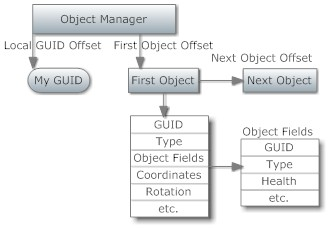
\includegraphics[scale = 0.65]{objmanalone.jpg}	
\caption{A representation of the object manager}
\label{objalone}
\end{figure}

%Discuss ASLR, Warden. Explain how objects are related to each other in WoW memory space. Also mention how they change with every update. Explain how to reverse engineer the client to get this structure when its updated briefly and where it is available online after its updated.
\lstset{language=c}
\lstset{basicstyle=\small}
\lstset{backgroundcolor=\color{listinggray},rulecolor=\color{blue}}
\lstset{linewidth=\textwidth}
\lstset{commentstyle=\textit, stringstyle=\upshape,showspaces=false}
\lstset{frame=trBL,frameround=tttt}


\section{Tracking Software Logic}
In this section, the logical flow of the tracking software implemented in this project is discussed in detail. The features needed by the program is first discussed, before giving an overview of the program  in the form of a flow diagram, with each of the more complex blocks being discussed in more detail further on in the section.

\subsection{Features Needed}
When designing software from scratch, it is helpful to first imagine a scenario of a user using the software to determine what features the software needs to provide. The software also needs to anticipate any actions that an unknowing user could do to prevent errors from occurring. The following short scenario reveals a few things the software should anticipate, as well as the features that are needed.

When a user wants to gather location data in WoW with this software, his first steps would be to start both the tracking software and WoW. The tracking software will only be able to track players once the user has entered the game world fully however, so a message should be displayed informing the user to click a reload button once the game world has been entered. The first potential problem the user could have is that the tracking software window is hidden behind the game window. This suggests that an option is needed to keep the tracking software window always on top.

Now that the program window is in view and has been loaded fully, the user needs some assurance that the program is working correctly. For this purpose a graphical representation of the player and surrounding NPCs and players need to be shown. Some information about the character of the user and the characters' current target being displayed will also assure the user that the program is working properly. A function is thus needed that draws players or messages on a bitmap that is then displayed to the user.

The user should now be convinced that the program is working and would want to start using it for tracking purposes. The user might only want to capture location data at certain times, so the option to turn tracking on and off is needed. The tracking data can be used in many ways, but the most obvious way would be to plot traces of the movement data captured. It would be very convenient for the user to not only have the option of tracking players, but to also show the traces as they happen in real time as a visual representation of the players being tracked. The user would then want to save the data to files when the tracking is done, before exiting the program and WoW.

From this scenario it is determined that the software needs the following features:

\begin{itemize}
	\item A reload button in case the user opens the program too soon, or something goes wrong.
	\item An option to keep the tracking window on top of other windows.
	\item An option to start and stop tracking players.
	\item An option to show the traces of players as they move.
	\item A button to save the tracking data when the user is done tracking.
\end{itemize}

Some features are only realised as the program progresses. Using the software showed that the graphical representation of players can become unusable when too many players are cluttered together. A zooming feature was added to add space between players in cluttered areas. An option to hide names from the graphical representation was also added to cause less clutter. Figure~\ref{wowdar1} shows the final GUI for the tracking software.

\begin{figure}[htbp]  %maybe move figure to earlier in text.
\centering
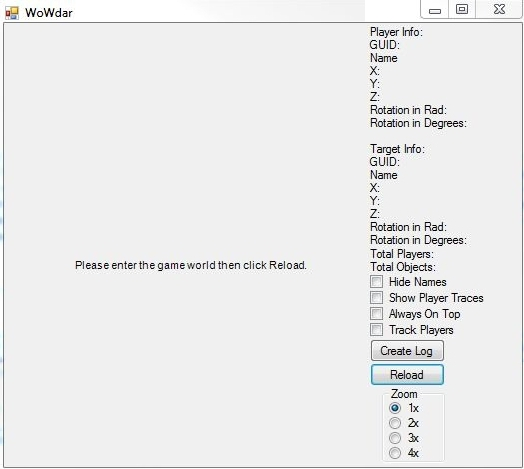
\includegraphics[scale = 0.65]{wowdar.jpg}	
\caption{The user interface of the tracking software program}
\label{wowdar1}
\end{figure}

\subsection{Initialisation}

The software needs to know when the user selects one of the features. To be able to do this a logical flow of events is needed in the software.

The first step for any software is to initialise the program. After initialisation the program needs to know if it loaded successfully or not, it also needs to let the user know this. The initialisation process of the program only involves loading the values of some needed global constants from the memory of the WoW client. The program then sets a flag true if the initialisation succeeded or false if it failed. The end of the code is then reached and the program stops temporarily.

The simplest way to describe the nature of the program is that it has to read values over and over again. This means that one block of code needs to be executed infinitely while the program is running, to keep the data up to date. To do this, a timer is needed. The timer is set to generate an interrupt every 10 milliseconds (ms) and to execute a block of code every time an interrupt is generated. 

Two flow diagrams are thus needed for this program, one for the initialisation and one for the code that gets executed every 10 ms. On overview of the initialisation code is shown in figure~\ref{init}.

\begin{figure}[htbp]  %maybe move figure to earlier in text.
\centering
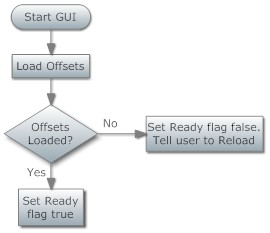
\includegraphics[scale = 0.65]{initover.jpg}	
\caption{An overview of the initialisation process}
\label{init}
\end{figure}

\subsection{Loading Offsets}

The Load Offsets block in figure~\ref{init} is a function that needs further explanation. The job of the Load Offsets function is to read a few values out of the WoW client software memory and to save it as global constants. These constants are needed by the code that executes every 10 ms to be able to access the object manager among other things.

The first problem this function has is that it needs access to the base address of WoW. The whole point of ASLR is to make sure that the base address is always different, so it needs to find another way to get the base. To get the base address of a process that uses ASLR, it is necessary for the process to be executed and loaded into memory first. Every process that is currently running is given a process identifier (PID) by the operating system to distinguish between different processes. The Load Offsets function searches through the list of running programs for one that is called WoW. Once it has the PID of WoW, C\# provides methods to get the base address of the process.

The Load Offsets function then adds a few different offsets to the base offset of WoW to get access to the following constants:
\begin{itemize}
	\item The base address of the object manager.
	\item The base address of the first object in the object manager.
	\item The GUID of the currently selected target.
	\item The GUID of the current character.
	\item The name of the current character.
\end{itemize}

The function then changes the labels on the GUI to show the name and GUID of the current character. The function returns true if all of this was done successfully. If any of the above steps failed however, the function informs the user that the Reload button must be clicked once the game world has been entered, and returns false. A flow diagram of the Load Offsets function is shown in figure~\ref{loadoff}.

\begin{figure}[htbp]  %maybe move figure to earlier in text.
\centering
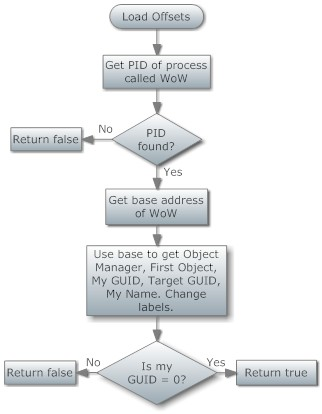
\includegraphics[scale = 0.65]{loadoff.jpg}	
\caption{A flow diagram of the Load Offsets function}
\label{loadoff}
\end{figure}

After the initialisation has taken place, the timer is started and after 10 ms the recurring code is executed for the first time. The program needs to be aware of any options chosen by the user, so a test is required to determine which options are selected. The user will see how the program reacts by the way that the user's character and other players and NPCs are sketched on the bitmap. It is thus important that the program reacts immediately when an option is changed.

\subsection{Recurring Code}

The first thing the recurring code needs to check is whether the initialisation was successful. If it was not, the user needs to be informed that the Reload button must be pressed with a message written on the bitmap. If the initialisation was successful, the program needs information that will determine how the players are drawn on the bitmap. This includes information such as the zoom level chosen and whether player traces must be shown or not. When the option to display traces is selected, the usual arrow used to display players is replaced by a thin line. All names are also hidden automatically in this view, and the bitmap is never cleared in order to keep previous traces of players. If the option is not selected however, the bitmap must be cleared to update the positions of all the players.

After checking which visual options are chosen, the program needs to get gather the necessary information to display all the characters in the game. It does this by using the global constant values which the initialisation process read from memory. 

Before the program goes on to read all the needed information from memory, a data structure needs to be defined in which all this data can be grouped together and saved. A class called WoW Object is created for this purpose, with fields to save the GUID, name, type, base address, object fields base address, health, coordinates and rotation in one data structure. Figure~\ref{wowobject} shows the WoW Object data structure.

\begin{figure}[htbp]  %maybe move figure to earlier in text.
\centering
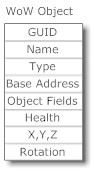
\includegraphics[scale = 0.65]{wowobject.jpg}	
\caption{The WoW Object data structure}
\label{wowobject}
\end{figure}


The program starts by saving the base address of the first object in a temporary variable to be used later. It also reads the GUID of the currently selected target again in case it changed since either initialisation or the previous 10 ms code execution. One of the global constants is the GUID of the local character. This GUID can be used to get the base of the local character object, which in turn grants access to the coordinates and rotation information. This information is then saved in a WoW Object for later use.

The next object of interest is our current target if one is selected. If no target is selected then the target GUID would be zero and the program would skip on. If there is a target currently selected however, then the GUID can once again be used to get the base address, which would grant access to the coordinates and rotation of the target. The target has more useful information which must also be read however, such as its type. Once the target has been classified as either human or NPC, the name of the target is read from memory, and all the information is saved in a WoW Object.

After the two special WoW Objects have been taken care of, the program needs to go through all of the other objects in the object manager and check the settings selected by the user each time to know what to do with the object. These objects are then drawn based on the selected settings one by one as the program loops through all the objects in the object manager.

After this process the program comes back to the two objects that are of special interest - the local character and the currently targeted character. The name and coordinates that was saved in WoW Objects for these two characters are then displayed on labels in the GUI, and the target and local player are sketched lastly on the bitmap, so that they would appear on top of the other objects if the other objects were close enough for them to overlap. Figure~\ref{10ms} shows an overview of this entire process.

\begin{figure}[htbp]  
\centering
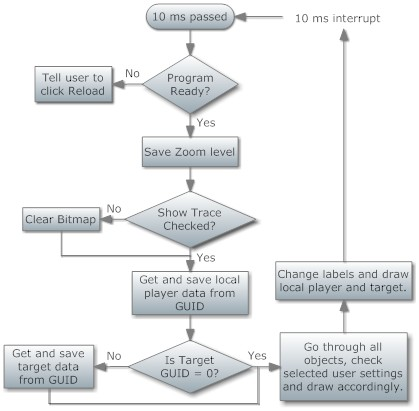
\includegraphics[scale = 0.65]{10ms.jpg}	
\caption{An overview of the code executed every 10 ms}
\label{10ms}
\end{figure}

Some of the blocks in figure~\ref{10ms} have more complex dynamics at work and need to be expanded into block diagrams of their own. When the program uses the globally constant local GUID to find the local player base, it is really calling a function to do this task. This function takes a GUID as an argument and returns the base of the object with the same GUID. It accomplishes this by using the globally constant value of the base address of the first object. 

It first compares the GUID received as argument to the GUID of the first object. If they match, the base address of the first object is returned. If they do not match, the algorithm moves on to the next object in the object manager and compares their GUIDs. This process is repeated until a match is found, or the end of the object manager is reached. If no match is found by the time the end is reached, zero is returned. Once the base address is returned, getting more information about an object is trivial. Figure~\ref{getbase} shows a flow diagram of this function.


\begin{figure}[htbp] 
\centering
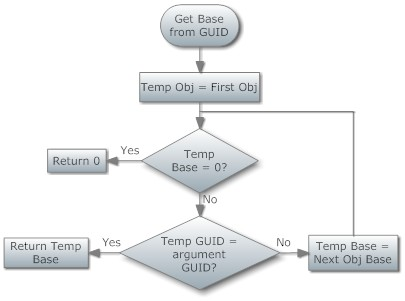
\includegraphics[scale = 0.65]{getbase.jpg}	
\caption{Flow diagram of get base by GUID function}
\label{getbase}
\end{figure}

\subsection{Cycling through the object manager}

The process of going through all the objects in the object manager, while checking which user settings are selected before drawing all the objects, was represented by a single block in figure~\ref{10ms}. This process is started by creating a WoW Object with the base of the first object. From the base, the other attributes of the object such as its GUID, coordinates, type and health is read by adding the appropriate offsets to the base address. The procedure for getting the name of an NPC is different from the one to get the name of a human player, so the type must first be analysed before the name is read from memory. Once all the attributes are saved in the WoW Object, the options selected by the user must be analysed so that the program knows what to do with the object. 

The first problem is that the current object might be the local player object. The local player is never tracked, and must be sketched last so that it appears on top of other objects, so it must be excluded from the start. Once the program ensured that the current object is not the local player, only two cases must be evaluated. The type of the object must be analysed, and any object that is not an NPC or human player must be discarded.

If the object is an NPC, then it must only be drawn if the show player traces option is not selected. When it is selected, only human players are of interest. The only other value of interest is the current health of the NPC to determine if the NPC is alive. If it is still alive, the NPC must be drawn in a plum colour, otherwise it must be drawn in grey to indicate that it is dead.

If the object is a human player the health must be checked first. The reason is that dead players are not tracked and will not create any traces, so they can be drawn immediately. If the player is alive the program must check whether the player must be tracked or not. If the ``Track Players'' option is checked then the player location data must be saved, otherwise the player must be drawn on the map. It is not necessary to check whether the player traces option is selected, as this is checked in the function that draws players on the bitmap. Figure~\ref{objects} shows a flow diagram of this procedure. To keep the flow diagram simple, the check for dead players was omitted, and it is implied that any object that is not a player or NPC is discarded.


\begin{figure}[htbp]  %maybe move figure to earlier in text.
\centering
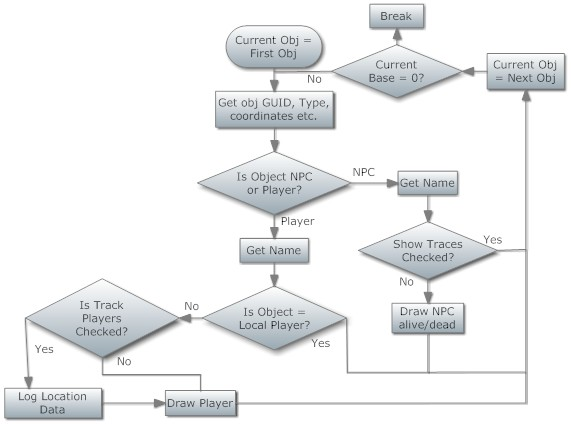
\includegraphics[scale = 0.65]{objects.jpg}	
\caption{Flow diagram of code that cycles through all objects}
\label{objects}
\end{figure}

%===================================================================================================================================================

\subsection{Logging information}
The end goal of logging the location data is to have the data saved for future use. This requires that the program either writes out the location data to a file every time it is read, or stores it in a data structure and writes it out when the user tells it to. Writing to a file takes more processing power than saving data in a data structure, which means that the first option would take more time to do than the second one, which could in turn cause the program to miss an update to the location data of a player.

For this reason a data structure is first needed to store all the relevant information in. For logging purposes the location of a unique player is important as well as the time when that player was at the specified position. The logs can then be used to completely reconstruct the movement of any player in exactly the same way that the player moved before, as well as in the same amount of time. To be able to save all this information, a structure called TimeAndPos is created with fields to save the location of a player and the time the player was at said location. 


The location of a player at a certain time is constantly changing, so all of this data needs to be stored in a list. This means that for every location and time pair of a player, a new structure must be created and stored. To order this information in a logical way, the structures are all placed in a list. The GUID of the player is not included in the TimeAndPos structure because the GUID of a player never changes and it would be a waste of resources to save the GUID over and over again.

To combine the list of movement data and the GUID of a player, a class called ObjArray is created. This class contains two fields: the GUID of one player, and a list called info, that contains all the TimeAndPos structures that form  a player's movement data in it.

The data structure described so far is suited to fully store the movement data of one player in WoW. There are many players that need to be tracked however, so the current data structure needs to be inserted into yet another list, which has one entry for every unique GUID.
A list called allObjects will be created for this purpose. Each entry in allObjects will thus contain a separate instance of the ObjArray class, with each one representing a unique player in the game world. The full data structure is represented schematically in figure~\ref{loggingstruct}.


\begin{figure}[htbp]  %maybe move figure to earlier in text.
\centering
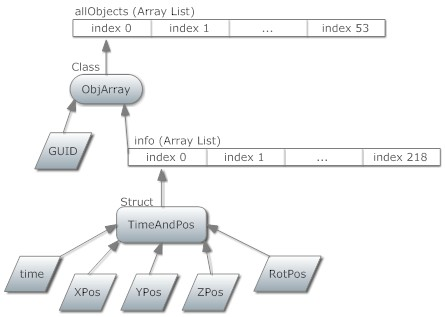
\includegraphics[scale = 0.65]{arrays.jpg}	
\caption{A schematic representation of the logging data structure}
\label{loggingstruct}
\end{figure}

The data structure shown in figure~\ref{loggingstruct} is needed to explain how the ``Log Location Data'' block in figure~\ref{objects} is executed.

At this point in the program, it has been determined that the ``Track Players'' checkbox has been checked and the location data needs to be logged. The program now has to save all the location data of the current player into the data structure shown in figure~\ref{loggingstruct}. The first step is to check if the list with all the objects in contains any data yet. 
If it does not, then that means that the current entry into it will be the first, and there is no need to search through it to see if the current player already has an entry in it. In this case the location data of the player and the current time must be added to the TimeAndPos structure, which must in turn be added into a new instance of the ObjArray class. The GUID of the player must then also be added to the ObjArray class, which is then inserted first into the list of all objects.

If there are already entries contained in the list, the program has to look through each entry in the list and compare the GUID contained in it to the GUID of the current object. If a match is found, the location data of the current object and the current time must be added to a new instance of the TimeAndPos structure, and added to the end of the info list. If the GUID is not found though, a new ObjArray instance must be created along with a new TimeAndPos structure. The data is then added into the TimeAndPos structure, which in turn is added to the ObjArray instance. The ObjArray is then lastly added into the allObjects list. Figure~\ref{logging} shows a flow diagram of this process.

\begin{figure}[htbp]  %maybe move figure to earlier in text.
\centering
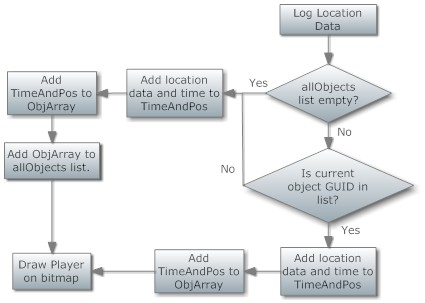
\includegraphics[scale = 0.65]{logging.jpg}	
\caption{Flow diagram of logging procedure}
\label{logging}
\end{figure}


At the moment all the data is saved in data structures, but as soon as the program is closed all this data will be lost immediately. The user needs to be able to choose when to save the data permanently. A button is provided in the GUI with the label ``Create Log''. When this button is clicked, all the data contained in the allObjects list needs to be saved to the computer in an ordered manner. A class called Log is created for this purpose. The class contains a method called WriteToFile, which takes the allObjects list as an argument and saves all the data contained in it to text files in the same directory as the executable file.

To distinguish between different players, the text file is named according to the GUID of the player. A possible name for a text file would be ``15543543556487.txt'' for example. This creates the potential problem that data from the same player might have been logged before, which could then be overwritten. To solve this problem the program will only append data to an existing file and create a new file if it does not exist  yet. All the data from previous logging sessions would  be unhindered with this method of saving. 

The data is written to the file with the date first, then the time of day accurate to 10 ms, then the X, Y and Z coordinates and finally the rotation. Each value is separated by a comma so that the data can easily be imported to programs such as MATLAB for further analysis.

%=====================================================================================================================================================

\subsection{Displaying player positions}


The virtual world in WoW is very large, and the Cartesian coordinates read from memory are usually large numbers. The only way to display characters from the game to the user in a intuitive and easy to understand way, is by displaying your own character in the center and then displaying all other characters relative to your own character. This is done by drawing all the characters on a bitmap, which is then displayed to the user.

The easiest way to sketch all the objects on one bitmap, is to create a function that takes the necessary data as arguments and returns a bitmap with the current player added to it. This function is then called after the data of each object in the object manager is read as can be seen in figure~\ref{objects}. When the end of the object manager is reached, the bitmap will be cleared unless showing player traces is enabled, and the process will repeat itself to show updated positions for all the players.

The following data is needed by the function:

\begin{itemize}
	\item The bitmap that must be drawn on. This bitmap must be a global variable.
	\item The colour to draw in.
	\item The Y-coordinate relative to your own Y-coordinate.
	\item The X-coordinate relative to your own X-coordinate.
	\item The rotation of the character in rad.
	\item The name of the player.
\end{itemize}

The coordinate system of a Bitmap object starts at zero in the top left corner, with the X-coordinate being more positive to the right, and the Y-coordinate being more positive to the bottom as shown in figure~\ref{bitmap}.

\begin{figure}[htbp]  
\centering
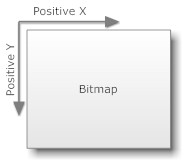
\includegraphics[scale = 0.65]{bitmap.jpg}	
\caption{The coordinate system of a Bitmap object}
\label{bitmap}
\end{figure}

This means that your character needs to be positioned at half the height and half the width of the bitmap in order to be displayed in the center. This offset needs to be added to the relative coordinates of any other characters as well in order to display correctly. The coordinate system used in WoW is inverted from the one used by bitmaps. In WoW the X-coordinate becomes more positive upwards, and the Y-coordinate becomes more positive to the right as illustrated in figure~\ref{wowcoord}.

\begin{figure}[htbp]  
\centering
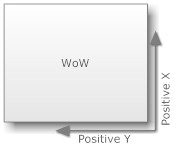
\includegraphics[scale = 0.65]{wowcoord.jpg}	
\caption{The coordinate system of WoW}
\label{wowcoord}
\end{figure}

If the X and Y-coordinates of the bitmap were switched around and then rotated 180 degrees, the two coordinate systems would be identical. For this reason, the X and Y-coordinates must be switched in the SketchPlayer function and the direction the character is looking in must also be rotated by 180 degrees. 

To rotate objects on a bitmap, a method called RotateTransform must be used. This method rotates an object by using the top left corner as its rotating axis, which creates a problem when the players need to be drawn in the middle of the bitmap. The only way to get around this problem is to first move the center point of the object, which is the relative coordinates in this case, to the top left corner. The object must then be rotated while it is in the corner by using the rotation information sent to the SketchPlayer function. After the object is properly orientated it must be moved back to its proper place. 

When these methods are used, it is technically the drawing coordinate system that is being moved around and rotated. This allows the function to move the coordinate system around before drawing the object on the bitmap, because once the object has been drawn it cant be changed without clearing the bitmap. The object is then only drawn after the drawing coordinate system is at the proper position. The program has to keep the user options in mind before drawing a player on the bitmap, by checking if the ``Show Traces'' option is selected. If it is, a line is drawn, otherwise an arrow is drawn.
The flow diagram of the SketchPlayer function is provided in figure~\ref{sketching}.

\begin{figure}[htbp]  
\centering
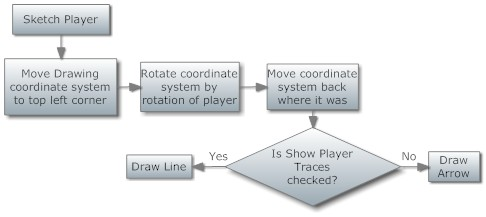
\includegraphics[scale = 0.65]{sketching.jpg}	
\caption{Flow diagram of the SketchPlayer function}
\label{sketching}
\end{figure}


%gaan nou in meer detail in oor die ander objects deel in, en dan meer, en meer. Maar eers get base by guid.

%\section{Memory Reading}
%
%In this section the procedure for accessing the memory of a process is discussed. This procedure is then expanded to include gathering the coordinates and other data from players in WoW. This knowledge was gained by studying similar open source projects that were done on previous versions of WoW, and applying modified versions of the same concepts to this project ~\cite{wradar, wowbot, wowradapp, wowradar}. 
%
%
%
%To be able to access the memory of a process, it is necessary for the process to be executed and loaded into memory first. Every process that is currently running is given a process identifier (PID) by the operating system to distinguish between different processes. The first step to accessing an open process is to get its PID. This can be done in C\# by using the Process.GetProcessesByName(String) method. 
%
%
%\lstset{language=c}
%\lstset{basicstyle=\small}
%\lstset{backgroundcolor=\color{listinggray},rulecolor=\color{blue}}
%\lstset{linewidth=\textwidth}
%\lstset{commentstyle=\textit, stringstyle=\upshape,showspaces=false}
%\lstset{frame=trBL,frameround=tttt}

%
%
%In the code, the Process.GetProcessesByName(string) method is called with the string ``wow'' as its argument. This returns an array of all processes with that name to the newly created wow process array. Usually only one instance of WoW is run on a computer at any one time, so the MainModule property of the first (and probably only) element in the array is assigned to the newly created ProcessModule object called ``wowModule''. Once we have the main module of the process, its simply a matter of assigning its BaseAddress property to a IntPtr object, and casting that object to an unsigned integer.
%WoWBase will now contain the base address of the WoW process.
%
%The .NET framework makes many of these types of operations easy to do, but there are open source libraries available that allows you to do these operations, and many others, with much less effort. The library used in this project is called ``BlackMagic'' and it makes process, thread and memory manipulation much easier and faster than it would normally be ~\cite{blackmagic}.
%The following code snippet shows how to get the  base address of the WoW process using the BlackMagic library.
%
%\begin{lstlisting}
%
%using System;
%using Magic;
%
%BlackMagic wow = new BlackMagic(); //create blackmagic object
%wow.OpenProcessAndThread(SProcess.GetProcessFromProcessName("Wow"))
%IntPtr baseWoW = wow.MainModule.BaseAddress;//Gets Base Address
%uint WoWBase = (uint)baseWoW;
%
%\end{lstlisting}
%
%This method is not all that much more efficient than the one using C\# libraries, but when it comes to memory reading, BlackMagic simplifies the process drastically. 
%
%When the needed information for each object is read from memory, the information needs to be stored in a structured way to make access to it easier. For this reason the WoWObject class is created with all the needed variables included. A code snippet of the WoWObject class is provided below.
%
%\begin{lstlisting}
%
%class WoWObject
%{
%   public ulong GUID = 0;
%   public String Name = "";
%   public short Type = 0;
%   public uint BaseAddress = 0;
%   public uint ObjectFields = 0;
%   public uint health = 0;
%   public float X = 0;
%   public float Y = 0;
%   public float Z = 0;
%   public float Rot = 0;
%}
%\end{lstlisting}
%
%Now that the base address of the process is stored and we have a class to store the needed values in, a few global constant values need to be read from memory and made available to the rest of the program. These include the base address of the object manager, the first object in the object manager, the GUID and name of your character, and the GUID of your characters' current target. The necessary offsets are all obtained from users who reverse engineered the WoW.exe file and posted their findings online, with the first and largest contributer mentioned as the source ~\cite{offsets}. The code needed to read the global constants from memory is listed below, with the relevant offsets included.
%
%\begin{lstlisting}
%
%uint ClientCon = 0;
%uint ObjectMan = 0;
%uint FirstObj = 0;
%
%WoWObject Me = new WoWObject();
%WoWObject Target = new WoWObject();
%
%//offsets for WoW 4.2.2.14545
%public enum ObjectManagerOff : uint
%{
%    clientConnection = 0x980558,
%    objectManager = 0x463C,
%    firstObject = 0xB4,
%    nextObject = 0x3C,
%    localGuid = 0xB8
%}
%    
%private Boolean LoadOffsets()
%{
%   ClientCon = wow.ReadUInt((uint)baseWoW 
%      + (uint)ObjectManagerOff.clientConnection);
%   ObjectMan = wow.ReadUInt(ClientCon 
%      + (uint)ObjectManagerOff.objectManager);
%   FirstObj = wow.ReadUInt(ObjectMan 
%      + (uint)ObjectManagerOff.firstObject);
%   Target.GUID = wow.ReadUInt64((uint)baseWoW 
%      + (uint)PlayerOff.LastTargetGUID);
%   Me.GUID = wow.ReadUInt64(ObjectMan 
%      + (uint)ObjectManagerOff.localGuid);
%   Me.Name = wow.ReadASCIIString((uint)baseWoW + 0x980598, 20);
%   
%   if (Me.GUID == 0)
%       return false;
%   else
%       return true;
%}
%    
%\end{lstlisting}
%
%It is clear from the code how easy and intuitive it is to read memory with the BlackMagic library.
%The constant values are used to gain access to all the objects in the object manager by cycling through them like a linked list. Even though the GUID of your character and your current target is already stored, the actual WoWObject of your character and current target which contains the location information is still in the object manager. A function is thus needed that takes a GUID as its argument and returns the base address of that object in the object manager. The function thus receives an unsigned 64-bit integer as argument, searches through all the objects in the object manager for an object with that GUID and then returns the base address of that object. The code that accomplishes this is shown below.
%
%\begin{lstlisting}
%
%public uint GetObjectBaseByGuid(ulong Guid)
%{  //start from first object
%   TempObj.BaseAddress = FirstObj;     
%
%	 //loop through all objects till right one is found
%   while (TempObj.BaseAddress != 0)    
%   {
%     try
%     {
%        TempObj.GUID = wow.ReadUInt64(TempObj.BaseAddress 
%           + (uint)ObjectOffsets.Guid, false);
%       if(TempObj.GUID == Guid)
%       {
%          return TempObj.BaseAddress;
%       }
%       TempObj.BaseAddress = wow.ReadUInt(TempObj.BaseAddress
%         + (uint)ObjectManagerOff.nextObject);    
%       //move on to next object
%     }
%     //must handle exception that can be thrown by blackmagic
%     catch (Exception)
%     {
%        return 0; //should never happen
%     }   
%   }
%  return 0;   //return 0 if nothing is found.
%}
%\end{lstlisting}
%
%A temporary object is created that takes on the value of the base address of the first object in the object manager. The offset needed to read the GUID of any object is then added to the base, and the GUID is read and compared to the GUID that was sent to the function. If the two GUID values are the same, the function returns the base address of the object. Alternatively the base address of the temporary object is changed to the base address of the next object in the object manager, and the procedure is repeated until the right object is found. If nothing is found, then zero is returned.
%
%This code is a good example of how to cycle through all the objects in the object manager, which needs to be done to get all the location information of all the players contained in it. Before the location information of other players are read however, the location of your own character is needed so that it is known where the other players are in relation to your own character. Getting this information is made easy by using the function listed above to get the base address of your character object, since the GUID is already stored. The code snippet that gets the rest of the relevant data from your character object is posted and explained below:
%
%\begin{lstlisting}
%  Me.BaseAddress = GetObjectBaseByGuid(Me.GUID);
%  Me.X = wow.ReadFloat(Me.BaseAddress + (uint)ObjectOffsets.Pos_X);
%  Me.Y = wow.ReadFloat(Me.BaseAddress + (uint)ObjectOffsets.Pos_Y);
%  Me.Z = wow.ReadFloat(Me.BaseAddress + (uint)ObjectOffsets.Pos_Z);
%  Me.Rot = wow.ReadFloat(Me.BaseAddress + (uint)ObjectOffsets.Rot);
%\end{lstlisting}
%
%The location information is stored as floats in WoW memory, and the Cartesian coordinate system is used for the X, Y and Z values, while the rotation float is stored in radians (rad). The location information of the current target is read in a similar fashion from memory and the code will thus not be reposted here. For any other object the reading process is slightly different however, since the type of the object must first be determined. The only objects that are relevant for displaying purposes are those of type three and four - NPCs and human players. Of those two types, only the human players will be tracked, but it is still useful to display positions of the NPCs for testing purposes. The code that reads this extra information from the WoWObjects follows:
%
%\begin{lstlisting}
%CurrentObj.GUID = wow.ReadUInt64(CurrentObj.BaseAddress 
%  + (uint)ObjectOffsets.Guid);
%CurrentObj.ObjectFields = wow.ReadUInt(CurrentObj.BaseAddress 
%  + (uint)ObjectOffsets.ObjectFields);
%CurrentObj.Type = wow.ReadShort(CurrentObj.BaseAddress + 0x14);
%CurrentObj.X = wow.ReadFloat(CurrentObj.BaseAddress 
%  + (uint)ObjectOffsets.Pos_X);
%CurrentObj.Y = wow.ReadFloat(CurrentObj.BaseAddress 
%  + (uint)ObjectOffsets.Pos_Y);
%CurrentObj.Z = wow.ReadFloat(CurrentObj.BaseAddress 
%  + (uint)ObjectOffsets.Pos_Z);
%CurrentObj.Rot = wow.ReadFloat(CurrentObj.BaseAddress 
%  + (uint)ObjectOffsets.Rot);
%CurrentObj.health = wow.ReadUInt(CurrentObj.ObjectFields 
%  + (uint)UnitFields.UNIT_FIELD_HEALTH);
%
%if (CurrentObj.Type == 3)    //NPC 
%{
%  CurrentObj.Name = MobNameFromGuid(CurrentObj.GUID);
%}
%if (CurrentObj.Type == 4)    //human player
%{
%  CurrentObj.Name = PlayerNameFromGuid(CurrentObj.GUID);
%}
%
%CurrentObj.BaseAddress = wow.ReadUInt(CurrentObj.BaseAddress 
%  + (uint)ObjectManagerOff.nextObject);
%
%\end{lstlisting}
%
%This code reads the object type, the object fields offset and then the health field contained in the object fields. The health field is read for displaying purposes, and to stop tracking players once they die. The method for getting the name of a player and a NPC is different, which is why different functions are needed to read that data. Those methods will be discussed later on in the text however. The relationship between all these fields are depicted clearly in Figure \ref{datastruct}.

%maybe add support for more than one wow process later
%Explain how to read from the game memory and to extract all the information needed. Also talk about the library used to do this, how it works and give credits to creator (shynd).

%\section{Tracking Software}
%In the previous section the code needed to access the location information for every object in the object manager was shown. Now that the program has a way of accessing all the location information, it needs ways to be able to log, display and save that information for future analysis. The program written for this project gives the user the option to track players, to hide object names and to show player traces. The programming behind these options will now be discussed in further detail. The different options available to users is shown in Figure \ref{wowdar}.
%
%\begin{figure}[htbp]  %maybe move figure to earlier in text.
%\centering
%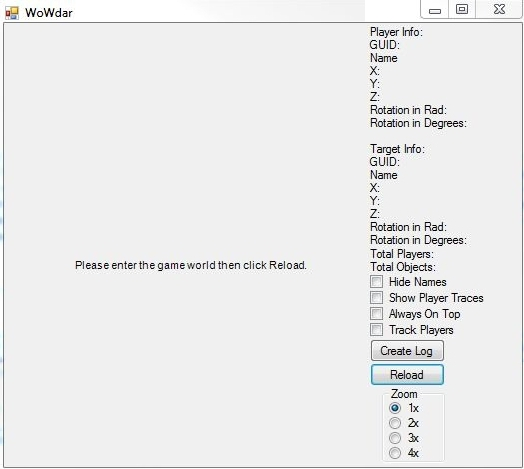
\includegraphics[scale = 0.6]{wowdar.jpg}	
%\caption{The user interface of the WoWdar tracking program}
%\label{wowdar}
%\end{figure}
%
%%Explain how the tracking software works briefly
%
%\subsection{Logging information}
%To be able to properly log the location information of players, a data structure is first needed to store all the relevant information in. For logging purposes the location of a unique player is important as well as the time when that player was at the specified position. The logs can then be used to completely reconstruct the movement of any player in exactly the same way that the player moved before, as well as in the same amount of time. To be able to save all this information a struct with the relevant fields mentioned above is created as follows:
%
%\begin{lstlisting}
%public struct TimeAndPos
%{
%  public DateTime time;
%  public float XPos;
%  public float YPos;
%  public float ZPos;
%  public float RotPos;
%}
%\end{lstlisting}
%
%The DateTime class allows the program to get and save the current time of the PC to the accuracy of a few milliseconds (ms). The time and location of a player will be changing constantly though, so all of this data needs to be stored in a list. The GUID of the player is also not included in this struct. The reason for that is that this struct will be in a list that will be growing constantly with updated information, while the GUID of a player will remain constant. Saving the GUID over and over again would be a waste of resources. A class with the name ObjArray is created to solve this problem. This class contains two fields in it: an unsigned 64-bit integer to store the GUID in, and an ArrayList object called info. The program reads the memory of WoW every 10 ms to update the location information of the objects in the object manager. Every time new information is read for a player, the program will store that information in a new instance of the TimeAndPos struct. This struct will then be added to the ArrayList called info, so that no information is lost. The ObjArray class is shown below:
%
%\begin{lstlisting}
%class ObjArray
%{
%  public ulong GUID = 0;
%  public ArrayList info = new ArrayList();
%}
%\end{lstlisting}
%
%There is still one problem that the data structure so far does not solve. The current setup only allows one GUID to be saved in the class. The info ArrayList contained in the class only has data that is relevant to the one GUID, so storing the other GUIDs in the ObjArray class is not an option. The solution is to create yet another ArrayList and to create a separate instance of the ObjArray class for each unique player. The ArrayList called allObjects will be created for this purpose. Each entry in allObjects will thus contain a separate instance of the ObjArray class, with each one representing a unique player in the game world. The full data structure is represented schematically in Figure \ref{loggingstruct}.
%
%
%\begin{figure}[htbp]  %maybe move figure to earlier in text.
%\centering
%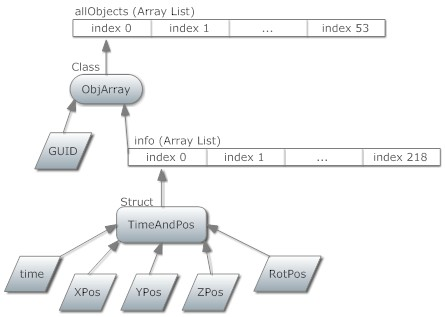
\includegraphics[scale = 0.6]{arrays.jpg}	
%\caption{A schematic representation of the logging data structure}
%\label{loggingstruct}
%\end{figure}
%
%The user is the one that controls whether the data must be logged or not. This is realised by only logging the data if the user selected the ``Track Players'' checkbox. When the checkbox is checked, the program will first test to see if the allObjects ArrayList contains any data. If it does not, then that means that the current entry into it will be the first, and there is thus no need to search through it for the current objects' GUID.
%
%If there are already entries contained in the ArrayList, the program has to look through each entry in the list and compare the GUID contained in it to the GUID of the object it is trying to add to the list. If they are the same, then the location information of the current object must simply be saved in a new instance of the TimeAndPos struct, and added to the end of the info ArrayList. If the GUID is not found though, then a new ObjArray instance must be created along with a new TimeAndPos. The TimeAndPos object is then added to the ObjArray instance, which is then added into the allObjects list. The relevant code section is posted below. This is after the program has confirmed that the current object is a human player that is not currently dead, and that the tracking checkbox has been checked.
%
%\begin{lstlisting}
%if (allObjects.Count <= 0)      
%{ //first entry into array
%  TimeAndPos temp = new TimeAndPos();
%  temp.XPos = CurrentObj.X;
%  temp.YPos = CurrentObj.Y;
%  temp.ZPos = CurrentObj.Z;
%  temp.RotPos = CurrentObj.Rot;
%  temp.time = DateTime.Now;       
%  ObjArray trackPlayer = new ObjArray();
%  trackPlayer.GUID = CurrentObj.GUID;
%  trackPlayer.info.Add(temp);
%  allObjects.Add(trackPlayer);
%}
%else                    
%{ //search through array for current player GUID
%  foreach(ObjArray tracking in allObjects)
%  {
%    if (tracking.GUID == CurrentObj.GUID) 
%    { //means current player GUID already in array
%      Found = true;
%      TimeAndPos temp = new TimeAndPos();
%      temp.XPos = CurrentObj.X;
%      temp.YPos = CurrentObj.Y;
%      temp.ZPos = CurrentObj.Z;
%      temp.RotPos = CurrentObj.Rot;
%      temp.time = DateTime.Now;
%      tracking.info.Add(temp);
%    }
%  }
%  if (!Found) //item not found in list, add it to list
%  {
%    TimeAndPos temp = new TimeAndPos();
%    temp.XPos = CurrentObj.X;
%    temp.YPos = CurrentObj.Y;
%    temp.ZPos = CurrentObj.Z;
%    temp.RotPos = CurrentObj.Rot;
%    temp.time = DateTime.Now;      
%    ObjArray trackPlayer = new ObjArray();
%    trackPlayer.GUID = CurrentObj.GUID;
%    trackPlayer.info.Add(temp);
%    allObjects.Add(trackPlayer);
%  }
%  else
%  {
%     Found = false;  //reset value for next object
%  }
%}
%\end{lstlisting}
%
%At the moment all the data is saved in data structures, but as soon as the program is closed all this data will be lost immediately. The user needs to be able to choose when to save the data permanently. A button is provided in the user interface (UI) with the label ``Create Log''. When this button is clicked, all the data contained in the allObjects ArrayList needs to be saved in text files on the computer in an ordered manner. A class called Log is created for this purpose. This class contains a method called WriteToFile in it. This method takes an ArrayList as an argument and saves all the data contained in it to text files in the same directory as the executable file.
%
%To distinguish between the different unique players, the text file is named according to the GUID of the object whose location information will be saved in it. An example name for a text file would thus be ``15543543556487.txt''. This creates the potential problem that data from the same player might have been logged before, and that data might then be overwritten. To solve this problem, the AppendText method of the File class in C\# is used. This method creates a file if it does not exist yet, and simply appends text to the end of the file if it does exist. All the data from previous logging sessions would thus be unhindered with this method of saving.
%
%The reason that the data is not saved to a text file every time new data arrives is that the writing operation takes much more central processing unit (CPU) processing time than adding the data to an ArrayList does. The code that saves the data to text files is shown below:
%
%\begin{lstlisting}
%public void WriteToFile(ArrayList datalist)
%{
%  foreach(ObjArray obj in datalist)
%  {
%    using (StreamWriter w = File.AppendText(obj.GUID + ".txt"))
%    {
%      foreach(TimeAndPos data in obj.info)
%      {
%        w.WriteLine(data.time.ToString("yyyy/MM/dd,HH:mm:ss.ffff") 
%        + "," + data.XPos + "," + data.YPos + ","+ data.ZPos + "," 
%        + data.RotPos);     //write data to log file
%      }
%      w.Flush();  //write and clear all buffered text
%      w.Close();  //close file
%    }
%  }
%}
%\end{lstlisting}


%moet dalk die kode uithaal later as daar min plek oor is (of verkort)
%Explain how the information is logged and saved for future use.
%Mention program that can read logs and refer to proper chapter.

%\subsection{Displaying player positions}
%The virtual world in WoW is very big, and the Cartesian coordinates read from memory are thus often big numbers. The only way to display characters from the game to the user in a intuitive and easy to understand way, is by displaying your own character in the center and then displaying all other characters relative to your own character. This is done in this project by making use of the Graphics class provided by C\#, and using it to draw on a Bitmap object which is then displayed to the user by using a picture box to display the bitmap.
%
%The easiest way to sketch all the objects on one bitmap is to create a function takes the necessary data as arguments and returns a bitmap with the current player added to it. This function can then be called after the data of each object in the object manager is read. When the end of the object manager is reached, the bitmap will be cleared and the process will repeat itself to show updated positions for all the players.
%
%The following data will be needed by the function as arguments:
%
%\begin{itemize}
%	\item The bitmap that must be drawn on.
%	\item The colour to draw in.
%	\item The Y-coordinate relative to your own Y-coordinate.
%	\item The X-coordinate relative to your own X-coordinate.
%	\item The rotation of the character in rad.
%	\item The name of the player.
%\end{itemize}
%
%The coordinate system of a Bitmap object starts at zero in the top left corner, with the X-coordinate being more positive to the right, and the Y-coordinate being more positive to the bottom as shown in Figure \ref{bitmap}.
%
%\begin{figure}[htbp]  %maybe move figure to earlier in text.
%\centering
%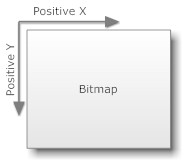
\includegraphics[scale = 0.6]{bitmap.jpg}	
%\caption{The coordinate system of a Bitmap object}
%\label{bitmap}
%\end{figure}
%
%This means that your character needs to be positioned at half the height and half the width of the bitmap in order to be displayed in the center. This offset needs to be added to any other characters relative coordinates as well to display correctly. The coordinate system used in WoW is a inverted from the one used by bitmaps however. In WoW the X-coordinate becomes more positive upwards, and the Y-coordinate becomes more positive to the right as illustrated in Figure \ref{wowcoord}.
%
%\begin{figure}[htbp]  %maybe move figure to earlier in text.
%\centering
%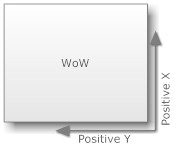
\includegraphics[scale = 0.6]{wowcoord.jpg}	
%\caption{The coordinate system of WoW}
%\label{wowcoord}
%\end{figure}
%
%If the X and Y-coordinates of the bitmap were switched around and then rotated 180 degrees, the two coordinate systems would be identical. For this reason, the X and Y-coordinates must be switched in the SketchPlayer function. The direction the character is looking in must also be rotated by 180 degrees. This is done using the RotateTransform method of the Graphics class. This method rotates the drawing coordinates from the left top corner of the bitmap. 
%
%This method also uses degrees as an argument, so the radians first needs to be converted to degrees. After this conversion is made, the coordinates where we want to draw must be moved so that it is in the top left corner first. The coordinates must then  be rotated by the degrees specified in the argument and moved back to its intended position before being drawn. It is in essence the coordinate axes that is being moved around and rotated. If the character in WoW is looking in the direction of 0 degrees, it should be displayed as an arrow pointing upwards, but since the coordinate system of the bitmap is rotated by 180 degrees, an arrow pointing downwards will be drawn to flip the image by 180 degrees. 
%
%The coordinate axes has already been rotated and the image should thus be displayed correctly relative to the center of the bitmap where your character is. An arrow is drawn by using the DrawLine method four times to draw an arrow shape.
%Some relevant code snippets are shown below to illustrate how this is done in the program.
%
%\begin{lstlisting}
%private Bitmap SketchPlayer(Bitmap img, Color UnitColor, 
%  float Ypos, float Xpos, float Rotation, string strName)
%{
%  Graphics G = Graphics.FromImage(img);  
%  Pen NormalPen = new Pen(UnitColor, 2F);
%  Rotation = RadToDeg(Rotation);
%  G.ResetTransform(); //Resets the coordinate system
%  G.TranslateTransform(-Xpos, -Ypos, 
%  System.Drawing.Drawing2D.MatrixOrder.Append);
%  
%  G.RotateTransform(-Rotation, 
%  System.Drawing.Drawing2D.MatrixOrder.Append);          
%  //rotate counterclockwise at origin
%  //move back to drawing coordinates
%  G.TranslateTransform(Xpos, Ypos, 
%  System.Drawing.Drawing2D.MatrixOrder.Append);
%
%  G.DrawLine(NormalPen, Xpos - 2, Ypos + 2, Xpos, Ypos - 6);
%  G.DrawLine(NormalPen, Xpos + 2, Ypos + 2, Xpos, Ypos - 6);
%  G.DrawLine(NormalPen, Xpos, Ypos - 2, Xpos, Ypos - 6);
%  G.DrawLine(NormalPen, Xpos - 2, Ypos +1, Xpos + 2, Ypos +1);
%
%  G.Dispose();
%  NormalPen.Dispose();
%  return img;
%}//end sketchplayer 
%\end{lstlisting}


%Explain how the positions are displayed in real time
%could include more detailed discription with more pictures
\subsection{Zoom level}
Different zoom levels are provided in the GUI. Figure~\ref{10ms} shows that the chosen zoom level is saved in the beginning of the program. To implement the zoom level, the relative X and Y-coordinates of the players and NPCs are multiplied by the amount of the chosen zoom level. 
The positions of the displayed players are all relative to you as a center point, so multiplying the distance to the center with the zoom level is all that is required for the different zoom levels to work.

\subsection{Showing Traces} %remember to mention target player traces
The point of showing player traces is to get a quick idea of what the movement data represents. It is implemented by first clearing the bitmap of the normal view where players and NPCs are represented as arrows, and then drawing players only as lines from then on. NPCs are also not drawn anymore, to keep the traces relevant to the movement of human players only. Each time the position of a player gets updated, the SketchPlayer function draws a new line to represent to position of the player. Since the bitmap is no longer cleared while this option is selected, a trace is formed as the player moves around.

One setback of using this method of displaying traces is that your character has to stand completely still for the traces to display correctly. The zoom level can also not be changed while the traces are shown, and must be chosen beforehand. 

A possible way to overcome this problem is to log all the location data of the players when the ``Show Traces'' option is checked. The bitmap can then be redrawn with every cycle through the object manager, allowing your character to move around freely while the traces are still shown. The reason that this is not implemented in the program is that the location data increases exponentially, and having to draw all those traces over and over again slows the program down exponentially. Within seconds the program takes long enough to draw the new traces that new location data is missed. The best way to show traces in real time is thus the method described above with the prerequisite of your character standing still while the traces are formed.

The location data of all the players can still be logged while the traces are being shown, so if your character does move around, the ruined traces can still be reconstructed from the logs.


%Explain how traces are shown in real time.




\section{Log Reading Program}

The logs that are created by the tracking software have a lot of useful information in them that can be extracted and analysed in detail at any time. It would be convenient to be able to see a quick representation of the data contained in the log files without needing to do much effort. For this reason a program needs to be created that can read the logs created by the tracking software and draw traces from them. 

This program needs the ability to select a single log file and to display the player trace contained within it for individual trace analysis. It must then be able to overlay additional traces on the one already shown. This is done by only clearing the bitmap when the user clears it by clicking a button. Every trace is then added to one bitmap without clearing it first, using the same SketchPlayer function used in the tracking software.

In densely populated areas, it is easy to capture the movement data of more than 60 players. Adding 60 logs one by one to the log reading program would take too long, so an option to draw all the traces in a folder is needed. A button is added that enumerates through all the log files in the same folder as the executable file and draws all the traces contained in the logs.


%To accomplish this, the standard open file dialog object of the .NET framework is used. This object then opens the standard file dialog of Windows and filters any file that is not a text file. The user can then select the log file to be displayed and click on a button to draw the player trace. Traces from other log files of other players can then be added one by one, either being displayed alone or overlapping the other traces, depending on the users choice. An option is also needed to draw all the traces in the same folder as the executable file, since there can be a very large amount of traces which would take long to add one by one.

%This is easy to do by enumerating through all the text files in the same directory, extracting the log information and using the same SketchPlayer function used in the WoW Tracking program. The biggest problem is how to extract the right information from the log files, and to test to some extent for invalid log files. This problem is solved by structuring the log file in such a way that it is easy to extract the correct information if it is a viable log file, and that it is unlikely for any other file to contain the same structure. 

%A correctly formatted log file should contain five commas on each line, each separating values from each other. Programs such as MATLAB can easily import values that are comma separated, which is why this structure was chosen. The log reading program then reads a line from the text file and splits the string at each comma. The values are then parsed according to the structure that the log file was saved in, and those values are sent to the SketchPlayer function.

%The code that parses the log files is shown below:
%
%\begin{lstlisting}
%using (StreamReader sr = new StreamReader(ChosenFile))
%{
%  String line;
%  while ((line = sr.ReadLine()) != null)
%  {
%    string[] info = line.Split(delimiter);
%    if (info.Length == 6)
%    {
%      X = float.Parse(info[2]);
%      Y = float.Parse(info[3]);
%      Rot = float.Parse(info[5]);
%
%      TraceBitmap = SketchPlayer(TraceBitmap, Color.Blue, 
%       (Xref - X)*fZoom + iTraces.Width/2, (Yref - Y)*fZoom 
%        + iTraces.Height / 2, Rot);
%      SaveBitmap = SketchPlayer(SaveBitmap, Color.Blue, 
%       (Xref - X)*fZoom + SaveBitmap.Width/2, (Yref - Y)*fZoom
%        + SaveBitmap.Height / 2, Rot);
%    }
%  }
%}
%\end{lstlisting}

The data contained in all the log files can come from a large area which might not fit in the display window of the program. The program does have the ability to zoom both in and out, but it might become hard to clearly see the traces if zoomed out too much. The solution to this problem is to allow the user to export the trace information to a bitmap file the size of the user's choice. This function allows the user to create a file of up to 10 000 mega pixels in size, which should be large enough to show any trace contained in the logs. The traces are drawn with the first location received chosen as the center point. The GUI of the log reading program is shown in figure~\ref{wowtraces}.%An example of a trace made in a dungeon being drawn is shown in Figure \ref{wowtraces}.

\begin{figure}[htbp]  %maybe move figure to earlier in text.
\centering
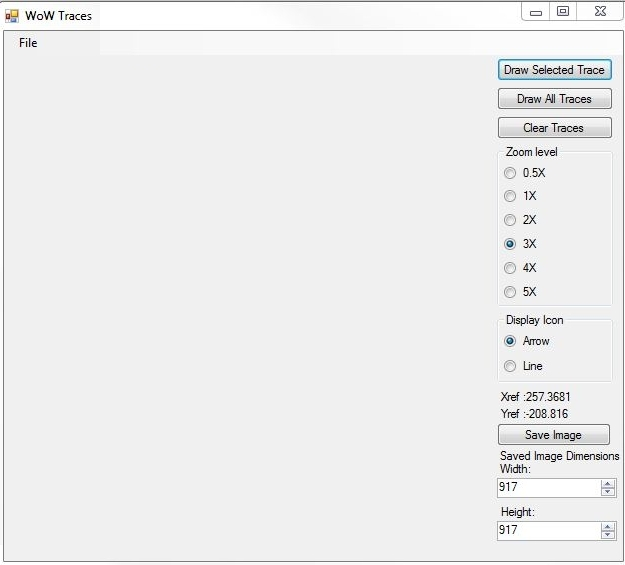
\includegraphics[scale = 0.8]{wowtraces1.jpg}	
\caption{The GUI of the log reading software}
\label{wowtraces}
\end{figure}


%Explain how the log reading program works. This could be a separate chapter?

%\section{Testing the Software}
%Several tests need to be done to ensure that the tracking software gathers accurate location data. This is done by going in game and comparing where NPCs and players are seen to where the software says they should be. This will give a general overview of whether the software works, but further testing is needed. Two characters need to log into the world simultaneously with each of them using the software. The coordinates of one character should be exactly the same on the two programs. The traces must then be tested by moving the character around and seeing if the trace on the other players tracking software reflects the same movements made. The data must then be logged, and the log reading program tested by redrawing the trace and seeing if it looks the same. 
%
%Larger scale testing then needs to be done by going into a capital city and capturing data and showing traces. The traces should then be compared to the layout of the city to see if the movement data makes logical sense. This is all done in chapter~\ref{results}. 

%Explain tests done to ensure that the software works as expected. Show proof and explain inconsistencies and mention latency.
\chapter{Results and Comparisons}
\label{results}

In chapter~\ref{ch5}, the details of how the player tracking software works were discussed. In this chapter, the strategy for analysing the database discussed in chapter~\ref{database} as well as the additional tests are executed. Tests to determine the accuracy and reliability of the player tracking and log reading software  are also executed. The data from the results are then collected and analysed. The results are compared to the expected behaviour, and any irregular behaviour is explained. This is done in separate sections, one for the database analysis and one for the player tracking software analysis.

%Explain that the tests done, data collected and results gotten will be discussed for both database analysis and player tracking software in this chapter in different sections.


\section{Database Analysis}
To analyse the database, it is of interest to determine the following:

\begin{itemize}
	\item Which actions in the game generate queries.
	\item How many queries each action generates.
	\item The average amount of queries from a gaming session.
	\item How much queries increase with more players in the game world.
	\item Which queries are the most frequent.
	\item The inter arrival time of the most frequent queries.
	\item The queries that take the longest amount of time to execute.
	\item How the server responds when many players are logged in concurrently.
\end{itemize}

This data is then analysed to determine the data storage and retrieval behaviour of the server, as well as its behaviour during a typical gaming session of both one and many players.

\subsection{Database Tests}
At first the strategy described in chapter~\ref{datastrategy} was executed to determine which actions in the game generates which queries from the server. The queries generated by the server being started were also analysed. 

To test how queries are generated during typical gameplay, the game was played for three hours with one player logged in. The player did quests and upgraded skills and started professions as any normal player would do. This process was repeated a few times with different gameplay times and using different characters of different classes and races.

After the game was played with a single player, bots were added to simulate multiple players in the game world as was mentioned in chapter~\ref{further}. The bots were also selected as characters from different races and classes to make the queries generated as diverse as possible. The bots follow a predefined path, leaving the path to kill mobs of interest when the mobs come into range. They then looted the mobs and tried to get back onto the path they were following. 

This behaviour often caused bots to run into trees, rocks or houses causing them to get stuck. The bots therefore had to be constantly monitored to ensure that they did not get stuck and that they completed the quests that they were given. All the loot also had to be manually sold when the backpacks of the bots were full. 

The bots also played the game for approximately three hours, with the expected result of the generated queries being roughly four times as much as when one human player played the game. This experiment was repeated to get more data for analysing purposes.

%Explain the tests done, how bots were added etc. 

\subsection{Data Collection}

The logs that were generated and saved after each action was performed as discussed in chapter~\ref{datastrategy} were collected and analysed to determine the server behaviour. The logs contained all the queries that were generated, and in the case of logs that took longer than the slow query logs' minimum time, the time each query took was also saved. This same data was collected during the typical gaming session done by one player, and again when the experiment was repeated with bots added. 

MONyog was also used to gather server status data every five minutes during the gameplay of these tests. This generated queries of its own, but these were ignored during analysis. The status data can not be saved in the same way that the logs can, so the data had to be used to create graphs immediately after each test was done, before new and irrelevant status data was captured by MONyog.



%The data required is information about which queries were made by the clients throughout the gaming session, as well as what time the queries were made and how long the queries took. The data was collected separately for the different tests done by activating the general and the slow query log. The logs were then saved and cleared after each test in order to start the next test with a clean log. MONyog was also used to gather server status data every five minutes during the gameplay. This generates queries of its own, but these were ignored when analysing the logs.
%
%The status data can not be saved in the same way that the logs can, so it had to be used to create graphs immediately after each test before new and irrelevant status data was captured by MONyog.


%Explain how data was collected and show results. 

\subsection{Results}
The results of the tests to determine which actions in WoW caused the server to generate queries was first analysed to better understand how the server responds to different actions, before the typical gameplay results were analysed.

\subsubsection{Wow Queries}

What was surprising after analysing the logs after each action was performed, was that most of the actions performed by the character did not generate immediate queries. The expected queries did however happen  a few seconds or even minutes after the action was performed. This suggests that the server saves all actions that will generate queries in variables at first. A queue of queries is then created that is executed either when the queue gets too full or after a certain interval. There are however certain actions that always generated immediate queries. This could mean that those queries are either big enough for the queue of queries to be considered full enough to be executed, or they are simply of higher priority and thus handled immediately. When these queries are executed however, the queries that were generated by performing other actions were still not executed, which rules out the theory of the server having a queue of queries that gets executed whenever it gets full.

Extensive testing was done to test this server behaviour, and after generating as much queries as possible with five clients logged in simultaneously, the queries still only happened after a counter of sorts triggered the queries to be made. This suggests that the server has a timer that generates an interrupt after a set amount of time has passed. This interrupt then causes the server to make all the queries from actions that have heaped up to the database. This is the equivalent of saving all the changes that have happened in the meantime.

It is sensible for the server to behave in this way, because the server has a lot of other things that it is responsible for, such as generating all the actions of the mobs and sending location information to all the clients and so forth. If every action that caused a change in game state generated an immediate query then the server would constantly be busy sending information to the database, causing lag in its normal and more important function of communicating with the client. This behaviour would become worse when more clients connect to the server, and the game would soon become unplayable. 

The following pattern was discovered by analysing hundreds of queries made to the database to ensure its legitimacy: there are two counters that generate queries constantly looping on the server side. The one counter generates a query to check if any of the players has sent mail to any of the other players every three minutes. This is the shorter of the two counters, which is understandable because other players could be waiting for the mail to be sent, which makes it a higher priority query.

The other counter generates a ``START TRANSACTION'' query every five minutes. This query starts a sequence of queries that save all the changes to all the characters that have happened in the past five minutes. This includes all new skills and spells learned, gold collected, quests accepted and completed and so forth. 

Table~\ref{queries} lists all the actions that were found to generate queries immediately, as well as the amount of queries that they generate. The queries generated by starting the ArcEmu server are also listed. Starting ArcEmu generates the largest amount of queries by far, but this should only happen once per week at a maximum, when servers are restarted for maintenance purposes.


\begin{table}[htbp]
  \centering
  \caption{List of actions in WoW that generate immediate queries}
    \begin{tabular}{lrlr}
    \addlinespace
    \toprule
    \textbf{Action in game} & \textbf{} & \textbf{Queries} & \textbf{Total time to execute} \\
    \midrule
    Starting ArcEmu &       & 1845 queries & 27.199 sec \\
    \midrule
    Logging in &       & 3 queries & 1.047 sec \\
    \midrule
    Creating a character &       & 18 queries & 0.765 sec \\
    \midrule
    Entering World &       & 23 queries & 0.597 sec \\
    \midrule
    Selling Items &       & 1  query & 0.056 sec \\
          &       & per item &  \\
    \midrule
    Dying &       & 2 queries & 0.059 sec \\
    \midrule
    Resurrecting &       & 1  query & 0.049 sec \\
    \midrule
    Logging Out &       & 76 queries & 0.078 sec \\
    \bottomrule
    \end{tabular}%
  \label{queries}%
\end{table}%


All of these actions in WoW are of high priority, which is why the server deems them important enough to break its usual cycle of only saving changes to the database every few minutes. Most of these actions only happen once per gaming session, or at the least they happen far less than other actions, so they should not have an adverse effect on the performance of the server.

The actions in the game that happen most frequently, like gaining skill points, levelling up and starting and completing quests are all processed at the same time, and only add one query per action to the list. Attributes like which spells a character knows and which items are in their backpacks are all both deleted and inserted into the database every five minutes with the ``START TRANSACTION'' query that happens. This will happen even if the character does nothing in that time. Analysing several logs revealed that the ``START TRANSACTION'' query generates approximately 66 queries for every player every 5 minutes when the player does nothing and is still low level. This sounds like a lot, but out of the 66 queries only 10 appeared in the slow query log, which means that 56 of them took faster than 0.000001 seconds to execute. 
The ``START TRANSACTION'' queries took a total of  0.095 seconds to execute.

\subsubsection{Typical Gameplay Analysis}

After analysing how the server handles queries, it is still of interest to determine if this behaviour persists when a player plays the game for long, and if the amount of queries multiplies when more players are added. The data of the one person playing and the bots playing was thoroughly investigated and it was found that the amount of queries and their size was mostly consistent with what was expected.

The game with one player in it will be referred to as game 1 from now on, and the game with four bots in it will be referred to as game 2.

The behaviour of the server suggested that queries should mostly happen every five minutes during gameplay, with the amount of queries from game 2 expected to be roughly four times as much as that of game 1.

From the time in the logs it was determined that game 1 lasted 205 minutes while game 2 lasted 218 minutes. There were 40 ``START TRANSACTION'' and 69 ``SELECT * FROM mailbox\_insert\_queue'' queries in game 1, and 157 ``START TRANSACTION'' and 73 ``SELECT * FROM mailbox\_insert\_queue'' queries in game 2. Table~\ref{botsres} shows the inter-arrival time of these queries for each of the queries in the two games.



\begin{table}[htbp]
  \centering
  \caption{Inter-arrival times for start transaction and mailbox insert queue queries}
    \begin{tabular}{lrr}
    \addlinespace
    \toprule
    \textbf{Queries} & \textbf{Game1} & \textbf{Game 2} \\
    \midrule

    START TRANSACTION & 5.125 min & 1.388 min \\
    \midrule
    SELECT * FROM mailbox\textbackslash \_insert\textbackslash \_queue & 2.971 min & 2.986 min \\
    \bottomrule
    \end{tabular}%
  \label{botsres}%
\end{table}%

As can be seen from table~\ref{botsres}, the start transaction query happened every 5 minutes as expected for game 1, and the other query also happened every 3 minutes as expected. In game 2, the one query behaved as expected, but the start transaction queries happened much more frequent than expected. This means that the server starts a separate timer for each character that logs into the game and saves their separate values to the database every five minutes. The reason that the inter arrival times are not exactly four times less than in game 1, is because it took a while to set up all the bots correctly, so the game was started with only one bot at first and the rest being added one by one every few minutes.

The logs of both games were processed next, to determine the top five most frequent queries and their inter-arrival times, as well as the queries that took the longest time to execute. Table~\ref{amount} shows the five most frequent queries and the amount of times they were executed during the games. The amount of times they were executed in game 2 is roughly three times as much as in game 1. The reason that it is not closer to four as expected is that the bots can not play the game as efficiently as a real player and therefore the amount of skills and so forth that the human player gained is much more than the bots could manage.

\begin{table}[htbp]
  \centering
  \caption{The amount of times the five most frequent queries were executed}
    \begin{tabular}{lrr}
    \addlinespace
    \toprule
    \textbf{Queries} & \textbf{Game 1} & \textbf{Game 2} \\
    \midrule
    INSERT INTO playerspells & 2313  & 7922 \\
    \midrule
    INSERT INTO playerskills & 548   & 1839 \\
    \midrule
    DELETE FROM playeritems & 421   & 1296 \\
    \midrule
    INSERT INTO playeritems & 237   & 908 \\
    \midrule
    DELETE FROM questlog & 192   & 517 \\
    \bottomrule
    \end{tabular}%
  \label{amount}%
\end{table}%

The inter-arrival times of the most frequent queries are shown in table~\ref{interamount}.

\begin{table}[htbp]
  \centering
  \caption{The inter-arrival times of the five most frequent queries}
    \begin{tabular}{lrr}
    \addlinespace
    \toprule
    \textbf{Queries} & \textbf{Game 1} & \textbf{Game 2} \\
    \midrule
    INSERT INTO playerspells & 0.089 min  & 0.027 min \\
    \midrule
    INSERT INTO playerskills & 0.374 min   & 0.118 min \\
    \midrule
    DELETE FROM playeritems & 0.487 min   & 0.168 min \\
    \midrule
    INSERT INTO playeritems & 0.865 min   & 0.240 min \\
    \midrule
    DELETE FROM questlog & 1.067 min   & 0.412 min \\
    \bottomrule
    \end{tabular}%
  \label{interamount}%
\end{table}%

Comparing the general and slow query logs, there are 4590 queries in total in the general log of which 514 appear in the slow query log for game 1. The other game has  15286 queries in the general log of which 2017 appear in the slow query log. This means that in both cases, less than 15\% of the queries generated takes longer than 0.000001 seconds to execute.

The query ``INSERT INTO character\_achievement\_progress'' took 0.35 seconds to execute, which was the longest query present in game 1. These queries happen often, yet only one took this long, so the reason is most probably that the computer was busy processing some other application which made the query take longer. For game 2 the longest query was a SELECT query, executed when a player logged into the world, which took 0.641 seconds to execute. This happened while the computer was busy running 4 instances of the game, which would keep the processor occupied and explains this long query time.

MONyog sent queries to the database every five minutes to check its status and saved the results temporarily. These results were used to draw figures for both game 1 and game 2, which are shown and compared next. To make game 1 reflect the behaviour expected from a normal player and to show what happens when no players are logged into the game, the character was signed off for a 15 minute break in the middle of the total game time. This can clearly be seen in figures~\ref{diffqueries}, \ref{rowaccess} and \ref{totalqueries}.

\begin{figure}[htbp]
\centering
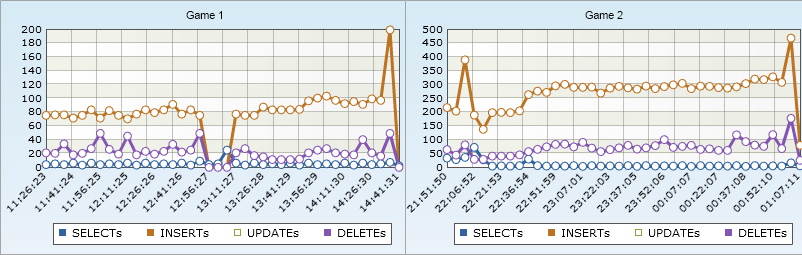
\includegraphics[scale = 0.75]{statecomp.png}	
\caption{Different queries over time for both games}
\label{diffqueries}
\end{figure}

Figure~\ref{diffqueries} shows the amount of different queries made during the two games. This result reflects the earlier result of the most frequent queries, with game 2 having roughly 3 times as much of each different query throughout the game.

\begin{figure}[htbp]
\centering
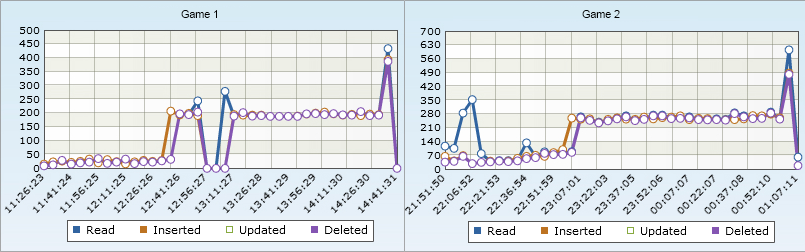
\includegraphics[scale = 0.75]{rowcomp.png}	
\caption{Different row access amounts over time for both games}
\label{rowaccess}
\end{figure}

Figure~\ref{rowaccess} shows the amount of rows that were accessed throughout the two games. The reason for the sudden jump in both games is that the character achievement progress query suddenly becomes more when the player levels up and learns more skills and spells. This query goes from accessing 0 rows, to 9 rows and then suddenly to 182 rows after levelling up and learning spells. The values in game 2 is not much more than in game 1 because the bots could not level up their characters enough to be able to do this. The rows being accessed by each of their queries stayed less than 20, and the only reason for the spikes that are seen in the graph is that the same character that was used in the first game was entered as a bot in the second game. This fact was taken into account when analysing the queries.

This is an interesting result to note however, especially since the size of the queries are of interest. The only way to judge the size of the query is by looking at the amount of rows accessed, of which all the other queries are dwarfed by the character\_achievement\_progress and the playerspells queries. The reason that they get so big is that a lot of new skills and spells can be learned by characters as they level up. These new skills and spells are probably each in a different row in their respective tables, causing the rows that need to be accessed to increase severely as the player progresses through the game.


\begin{figure}[htbp]
\centering
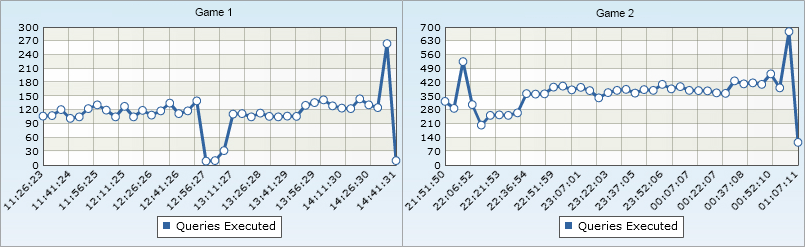
\includegraphics[scale = 0.75]{queriescomp.png}	
\caption{Total amount of queries executed for both games}
\label{totalqueries}
\end{figure}

Figure~\ref{totalqueries} shows the total amount of queries executed throughout the games. The value of game 2 is slightly more than 3 times as much as that of game 1 as expected. The reason it is not 4 times as much is once again that the bots can not play the game as efficiently as a human can, which resulted in less quests being completed and less skills and spells learned, which in turn resulted in less queries being executed.




%Discuss results, compare to what was expected and explain differences.

\section{Player Tracking Software Analysis}

To analyse and test the player tracking software, it is of interest to determine the following:

\begin{itemize}
	\item Whether the software reads the memory locations as expected.
	\item Whether the coordinates of the local player is the same as it is from another character using the software.
	\item Whether the traces created reflects true player movement data.
	\item Whether the log reading program recreates the traces correctly from logs.
	\item Whether the the tracking information in general is correct.
\end{itemize}

To determine this, tests need to be done and data collected.

\subsection{Player Tracking Tests}

The first test needs to determine whether the tracking software reads the memory of the WoW client properly. It was explained in chapter~\ref{ch5} how the data structure of WoW looks and how the software extracts the proper data from the memory. Figure~\ref{objalone} shows that a copy of the GUID of the local player is accessible directly from the object manager, which is then used to gain access to the object representing the local player, as shown in figure~\ref{getbase}. This same method is used to get access to the object representing the currently selected target. To test whether the tracking software reads the data structure correctly, and more importantly whether the data structure works as expected, a user must enter the game while using the player tracking software. The user must then select himself, making the local player the currently selected target. The software should then show the same name, GUID and coordinates for the local player and the target.

% Another copy of the GUID of the local player should be in the object that represents the local player in the object manager. These two values must be read from memory and compared to each other to test if the software reads the memory of the WoW client correctly. As an added test, the current player must be selected as the current target. This should create yet another copy of the GUID of the local player to be read and compared to the rest.

What needs to be tested next is whether the data shown graphically by the software reflects what the player sees in the game. The player must log into the game while using the software and compare the NPCs and other players it sees in the game to what NPCs and players the software says is around it. The names of the NPCs shown in game must also be compared to the names shown by the tracking software, as well as the data of the current target.

This test should prove that the data read on one computer is correct and consistent, but another test is needed to ensure that different players receive the same data. To test this, two different clients must log into WoW with different characters while using the tracking software. The two characters must then select each other as targets, and compare the information displayed about themselves and their targets by the software with each other. The target information from the one player should match the local player information of the other player exactly.

While having two payers logged in, the player tracing feature should be tested by enabling the feature with one player, and using the other player to move in a shape. The shape should then be reflected perfectly on the player tracking software. The other player should then be selected to make him a target, and another shape should then be drawn by moving, which should then be displayed in red.

Lastly, the usability and performance of the software must be tested when large amounts of players are tracked simultaneously. This test must be done in densely populated areas such as capital cities to get good test data. Traces should then be formed and compared to maps of the area to see if the movement data makes sense. 

%Briefly mention tests done to ensure program works again.

\subsection{Data Collection}
Data needs to be collected to prove that the software works accurately and as expected. To do this, the various tests mentioned need to be performed with screenshots of the game window and of the software being taken to prove that they were done and that they were successful. 

Data also needs to be collected about tracking large amounts of players. For this purpose the logs that the program creates must be collected and compared with what happened in the game to see if the data reflects what happened. The maps of the area must also be compared with traces of player movement data to see if the movement traces make sense and can be explained on the game map. This data must also be compared to what is happening in the game. 

Video footage of what happens in the game must be taken to compare to the results in the logs and the traces shown. This will allow any inconstancies to be explained by studying the video of the game. Screenshots and videos of the traces made in real time also need to be collected for comparison to traces recreated from logs, to see if the two are the same. After all this data has been collected, it needs to be analysed thoroughly to prove that the software works as expected.
%Mention how data was collected and show results

\subsection{Results}
\label{trackingresults}
It is of vital importance that the data structures of WoW are both understood correctly, and that the program reads them correctly. This was tested by selecting the local player, making it the current target. If everything works as it should, the software should have access to the local GUID, the target GUID and all the objects as shown in figure~\ref{test1}. The right objects must then be found by comparing the GUID that is already accessed with each object as is shown in figure~\ref{getbase}.


\begin{figure}[htbp]
\centering
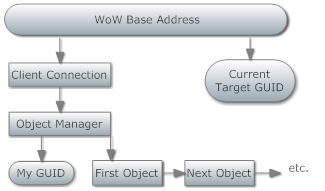
\includegraphics[scale = 0.75]{test1.png}	
\caption{The data structure that the player tracking software must use}
\label{test1}
\end{figure}

In WoW, the name, health, mana, level and a small picture of both the local player and the current target are shown in the top left corner of the UI as shown in figure~\ref{self2}. The local player is represented on the left, and the target on the right. Figure~\ref{self2} clearly shows that the local player is currently selected as the target in the game.

\begin{figure}[htbp]
\centering
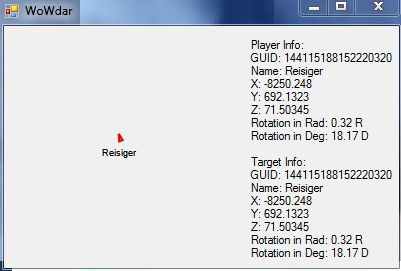
\includegraphics[scale = 0.75]{self1.png}	
\caption{Player tracking software with local player as target}
\label{self1}
\end{figure}

Figure~\ref{self1} shows the player tracking software with the local player selected as target. All irrelevant data has been edited out of the GUI in order to clearly show that the player and target information displayed in the tracking software are exactly the same. This includes the name, GUID, coordinates and rotation values.

\begin{figure}[htbp]
\centering
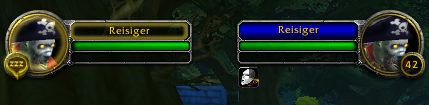
\includegraphics[scale = 0.75]{self2.png}	
\caption{The local player selected as the current target}
\label{self2}
\end{figure}

This is considered proof that the data structures of WoW works as explained. Next it needs to be confirmed that what the tracking software displays is reflected in the game world. To do this, an NPC is approached and targeted. The name, rotation and position of the NPC is compared to the same values displayed by the tracking software. Figure~\ref{target1} shows the local player standing in front of an NPC called Marshal McBride. A Stormwind Royal Gaurd can also be seen to the left. Both NPCs are looking in the opposite direction of the local target.

\begin{figure}[htbp]
\centering
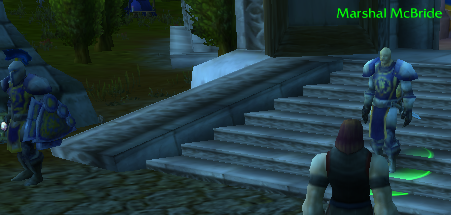
\includegraphics[scale = 0.75]{target11.png}	
\caption{An NPC is approached and targeted in the game}
\label{target1}
\end{figure}

Figure~\ref{target2} shows the tracking software view of the same moment in the game. The green arrow represents the local player, while the red one represents the current target, and all the plum ones are NPCs. Figure~\ref{target2} shows that the orientation of the NPCs, as well as their names, are an exact representation of what is shown in the game world.

\begin{figure}[htbp]
\centering
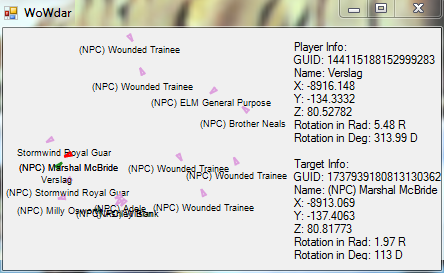
\includegraphics[scale = 0.8]{target12.png}	
\caption{Player tracking software showing an NPC being approached and targeted}
\label{target2}
\end{figure}

Now that it has been proved that the data received by one player using the software is consistent with what is represented in the game, it needs to be proven that different players using the software will also receive the exact same data. This is done by logging into the game with two different players, meeting each other in the game with the tracking software open for each player respectively, and selecting each other as targets. The target information of the one player should then be exactly the same as the local player information of the other player. Figure~\ref{ektarget2} shows the two players, Reisiger and Verslag,  meeting up in the game. 

\begin{figure}[htbp]
\centering
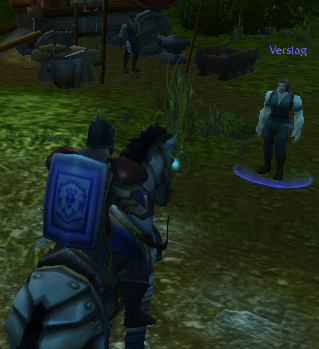
\includegraphics[scale = 0.75]{ektarget2.png}	
\caption{Two players meeting up in the game world}
\label{ektarget2}
\end{figure}

The information displayed by the tracking software of Reisiger is shown in figure~\ref{ektarget1}. The target information should be exactly the same as the local player information displayed by the tracking software of Verslag.

\begin{figure}[htbp]
\centering
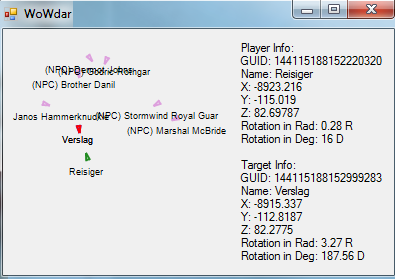
\includegraphics[scale = 0.8]{ektarget1.png}	
\caption{The tracking software display of Reisiger}
\label{ektarget1}
\end{figure}

The information displayed by the tracking software of Verslag is shown in figure~\ref{targetek1}. As can be seen from figures~\ref{targetek1} and \ref{ektarget1}, the information is displayed exactly as expected, with the name, GUID, coordinates and rotation being an exact replica of each other. This proves that the tracking software extracts and displays consistent and accurate values for all its users.

\begin{figure}[htbp]
\centering
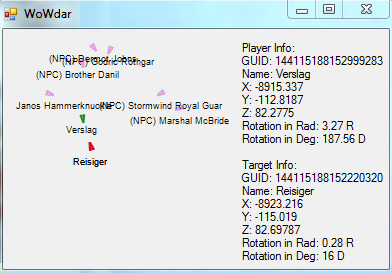
\includegraphics[scale = 0.8]{targetek1.png}	
\caption{The tracking software display of Verslag}
\label{targetek1}
\end{figure}

With the two players still logged in together, the show traces feature was tested by enabling the feature on one player's software, while the other player moved around in a specific way to form a shape. The shape should then be reflected on the player tracking software in blue. The player was then selected as the target before drawing yet another shape by moving. The trace made by a target should then be displayed in red. Figure~\ref{vierkant} shows the resulting display of the tracking software after the test was performed, with the square being made before the player was selected and the circle afterwards. The trace shows half a circle being formed unsuccessfully before the circle was then completed. This is an accurate representation of the player running into a tree before starting a circle without obstacles in the way. The circle is also not completely round, and the reason for this is that the player was riding a horse that galloped in that form when trying to run in a circle.


\begin{figure}[htbp]
\centering
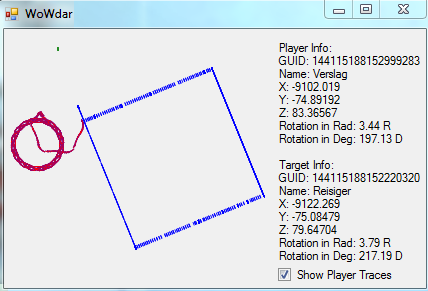
\includegraphics[scale = 0.75]{vierkant1.png}	
\caption{The traces made by moving around a player in certain shapes}
\label{vierkant}
\end{figure}

The accuracy of the log reading program also needs to be tested. To do this, the two players that are logged in simultaneously are used again. The one player moves in the shape of a triangle while the other player enabled both the tracking and the show traces features. The trace shown by the player tracking software must then be compared by the trace created by the log reading program when it reads the log created after the player moved in a triangle. Figure~\ref{tracetest1} shows the trace made by the tracking software, while figure~\ref{tracetest2} shows the trace made by the log reading software. The two forms are exactly the same, which proves that the log reading software can accurately read the logs and display the information they contain. It also proves that the player tracking software creates the logs properly, with no data being lost.

\begin{figure}[htbp]
\centering
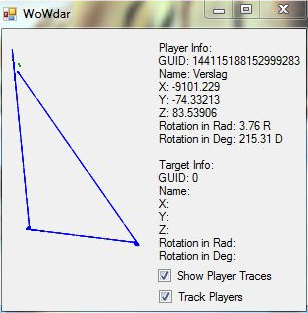
\includegraphics[scale = 0.75]{tracetest.png}	
\caption{The trace made by the tracking software}
\label{tracetest1}
\end{figure}

\begin{figure}[htbp]
\centering
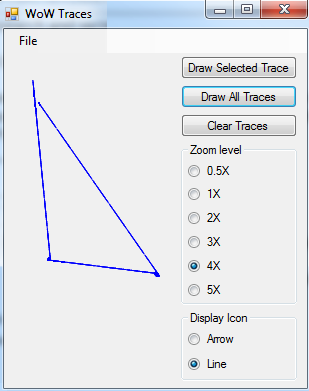
\includegraphics[scale = 0.75]{tracetest2.png}	
\caption{The trace made by the log reading software}
\label{tracetest2}
\end{figure}

Finally the performance and accuracy of the tracking software needs to be tested when there are many players to track. This is done by going into a city and enabling both the player tracking and the show traces features. The traces are then overlaid on a map to see if the movement data represented makes sense. Figure~\ref{stormtrace} shows the player traces captured in the city of Stormwind overlaid on the map of Stormwind. The auction house, bank and some flying mounts have been pointed out in figure~\ref{stormtrace}. A lot of traffic can be seen between the auction house and the bank. This is because players either buy an item at the auction house and then store it in the bank, or they get an item from the bank to sell at the auction house. The traces clearly follow the streets of the city, which can clearly be seen at the bridges, except in the case of flying mounts, which can fly over all the buildings.

\begin{figure}[htbp]
\centering
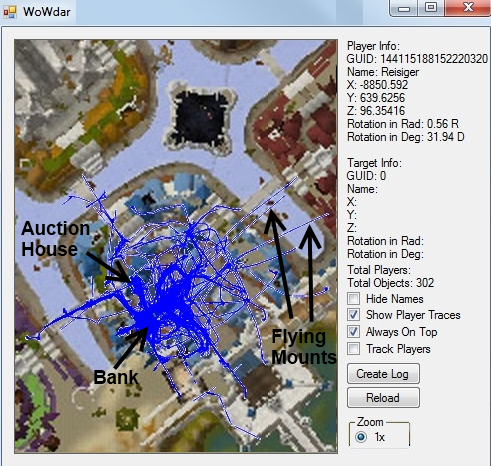
\includegraphics[scale = 0.75]{stormoverlay.png}	
\caption{Player traces overlaid on the map of Stormwind}
\label{stormtrace}
\end{figure}

Another test was done in the city called Undercity. The player traces overlaid on the map of Undercity is shown in figure~\ref{undertrace}. Undercity is an underground city as the name suggests, and therefore the movement of players with flying mounts are very limited. The green that can be seen is water, which players can enter if they want to, but it slows down movement. The rest of the map is mostly walkways, roads and walls. The trace shows that the players use the roads and walkways provided almost exclusively.

\begin{figure}[htbp]
\centering
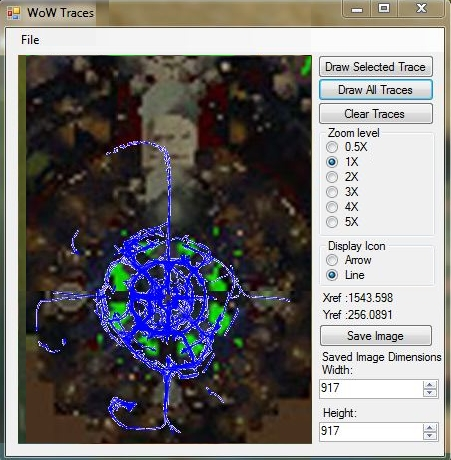
\includegraphics[scale = 0.75]{underlaycity.png}	
\caption{Player traces overlaid on the map of Undercity}
\label{undertrace}
\end{figure}

The traces shown in figures~\ref{undertrace} and \ref{stormtrace} contains no inexplicable movement data, which is considered proof that the player tracking software works efficiently and accurately in densely populated areas where a lot of players need to be tracked.


%Discuss results and compare with expected results and explain differences.


\chapter{Conclusion}
\label{conclusion}
In chapter~\ref{results}, the database of a private WoW server was analysed to determine when and why the server stores data. The accuracy and efficiency of the player tracking software was also tested. In this chapter, recommendations for improvements to the tracking software is made. The work done in the entire project is briefly reviewed and conclusions are made from the results presented in chapter \ref{results}. Possible future work is also discussed.

%Discuss future work and improvements that can be done on program. This can include overlaying map in real time as well as getting the scale right between game map and tracking data. Could also combine the log reading program with the tracking software program easily. Could improve on looks of program.  Think of other possible improvements and discuss them, and then write conclusion.

\section{Recommendations}

\subsection{Combine Programs}

This project saw the creation of tracking software that creates logs containing movement data of players in WoW. A separate program was written to read these logs and to display the movement traces of players that are contained within the logs. The log reading program also has the ability to export the traces to a bitmap image. A possible improvement would be to combine these two programs into one, where the program can track players, create logs and also read and display traces contained in logs and export the traces to a bitmap image.


\subsection{Overlay Map}

Overlaying player movement traces on a map of WoW gives a better idea of what the traces mean, as can be seen in chapter~\ref{trackingresults}. This overlaying was done by making the background of the bitmap invisible so that only traces can be seen, and then placing the program over an online map. It would be a convenient improvement if the tracking software was expanded to do this overlaying automatically for the user.


\subsection{Allow Movement While Tracing}

In the current player tracking software, traces can only be shown correctly in real time if the character of the user stands still while the traces are drawn. The reason is that the algorithm that was considered a solution to the problem caused severe lag in the program, making it unusable. A possible improvement would be to think up a better algorithm to solve this problem, and thus allow the character of the user to move around freely while showing movement traces of players.

\subsection{Include proper scale}

At the moment the display of the software represents players with relative distances, but it is sometimes hard to visualise how far the distance indicated by the software is in the game. A scale to show how distances in the game relate to distances in the software for each zoom level would be a good improvement. The area in which the server starts sending location data to the client can then also be indicated with a circle around the local player.

\section{Conclusion}

\subsection{Summary}
After providing an overview of the problem statement of the project and mentioning previous work done in similar projects, the aims in this project was clearly stated. This project can be seen as step one of a larger field of research, where a state persistent architecture for P2P MMOGs will be developed. In order to start the larger field of research however, it is necessary to characterise  the data storage methods used by a mature C/S MMOG, which can then be used as a benchmark for the P2P architecture. 

The movement of players in an MMOG also needs to be modelled in order to drive and test the performance of the P2P architecture, but since there has been very little research done in this field, data first needs to be collected about how players move in current MMOGs. Before this can be done however, a tool is first needed that can collect this data efficiently and accurately. Part of the aim of this project is thus the creation and thorough testing of such a tool. This tool can then be used in future projects to collect movement data from players and create mathematical models that describe the collected movement patterns. This will then in turn be used in the creation of a state persistent P2P architecture for MMOGs.

WoW is chosen as the MMORPG for which the tracking software will be developed, because it is currently the most popular MMOG in the world. The data storing characteristics of WoW must also be investigated to better understand how an MMORPG handles the data of such a large amount of players. Basic concepts of WoW are described that will help the reader understand the results obtained from the database analysis and player tracking software tests.

The methods that will be used to analyse the database and to get the player location information from the client software is described in detail before the actual analysis and testing takes place. The database is then analysed in detail with some interesting results that give a better understanding of how the server handles queries generated by clients. The player tracking software is tested for accuracy and efficiency next.

\subsection{Results}

From the database analysis the behaviour of the server can be characterised as follows:

The server has a lot of functions that it has to perform as described in chapter~\ref{mechanics}. For this reason it can not immediately save the data of any action that causes a change in the data of a certain client. The server divides the actions of players in the game into different categories of importance. The most important actions are listed in table~\ref{queries}, and they all cause the server to immediately execute a query to the database. The reason these actions are considered of such high importance, is that they cause large changes in the game state, and more importantly, if the data changed by them are not saved immediately it could create loopholes that players could use to cheat. If a player were to sell an item, without the server noting the change, and log out, then the data could be lost. This could create a situation where the player gets gold for the item without actually losing the item.

The server regards the action of players sending things to each other via mail as very important as well. A global counter is created that causes the server to execute queries created by sending mail every 3 minutes in the game.

Lastly the server creates a separate counter for each player that saves the minor changes made to the player's data every 5 minutes. This is the data that changes most frequently and saving it with every change would take up a lot of time of the server. The total time in executing this query is usually under 0.2 seconds. This time is most probably much less in the real server used by WoW, where the server and database would be optimised for these specific queries. The time to execute could quickly become long, with thousands of players logged in simultaneously, but Blizzard splits different areas in the game up to be serviced by different servers in order to prevent such a situation from happening. 

The most noteworthy queries size wise are queries that have to do with a player's progression through the game. The more skills, professions, spells, quests and levels a player gains, the more data needs to be saved. The different skills and so forth are also stored in different rows in the database tables, which results in more and more rows needing to be accessed. All of this data is summed up into two queries however, so it does not make a very noticeable difference in the big picture of all the queries that are executed.

The P2P architecture should strive to have the same data storage characteristics and performance as the one analysed in this text.

The accuracy and efficiency of the player tracking software is investigated next. Chapter~\ref{trackingresults} lists several results that proves that the tracking software is accurate in the following ways:

The tracking software both understands and reads the data structure of WoW correctly. This is shown by first discussing how the data structure is understood, and then testing it by reading values three values from different places in the client softwares' memory that should all be the same. The values are shown to be the same and correct. Next the name, position and orientation of an NPC is shown to be displayed the same by the tracking software than by the game client software. This proves that the tracking software shows an accurate representation of what is currently happening in the game world.

Two different players are then logged into the game concurrently and meet each other up with the software enabled for both players. The consistency of the data displayed by the software is proven by the different players seeing the same data being displayed by the software. The accuracy is then further proved by the software showing the traces of one of the players moving in both a square and a circle accurately in figure~\ref{vierkant}.

Both the accuracy of the logs being created by the software as well as the accuracy of the log reading program is proven by tracing the movement of a player moving in a triangle, and recreating the trace perfectly with the log reading software.

Lastly the efficiency of the tracking software is proven by tracking and showing the movement traces of more than 60 players in a capital city. The accuracy of the movement data is proven by overlaying the trace on a map of the area, showing how all the movement data makes logical sense.

%It is concluded that the player tracking software can efficiently and accurately trace a large amount of players without missing any important movement data. 

All the data movement data that was captured has been analysed to be correct but also incomplete. The reason for incomplete data is the result of one of three things:

\begin{enumerate}
	\item Latencies caused by slow Internet.
	\item Players becoming invisible, causing the server to stop sending their location data to clients.
	\item Players logging in and out, causing them to randomly appear and disappear into and out of the game world.
\end{enumerate}



It is concluded that the player tracking software can efficiently and accurately trace a large amount of players without missing any important movement data, with any missing data being because of the above mentioned reasons. The software can thus be used as a valuable tool to use in future work. Possible future work includes capturing a large amount of movement data and using that data to create models of how players move in an MMORPG. These models can then be used in turn to test the reliability and performance of P2P architectures for MMOGs. Finally a state consistent architecture for P2P MMOGs can be created. 


%Conclude that results indicate the program works and the database reacts as expected.
%\include{Chp-8}
%\include{Chp-9}
%\include{Chp-10}

%\backmatter%=========================================================

\bibliography{skripsie}

\appendix%====================================== =====================

\chapter{Project planning schedule}

%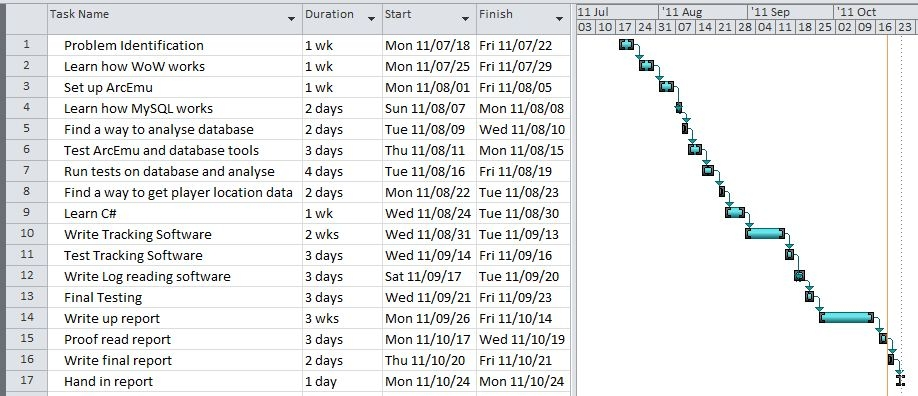
\includegraphics[angle = 90, scale = 0.8]{gantchart.jpg}
%Create a gant chart with planning schedule.

%\begin{figure}[htbp]  %maybe move figure to earlier in text.
%\centering
%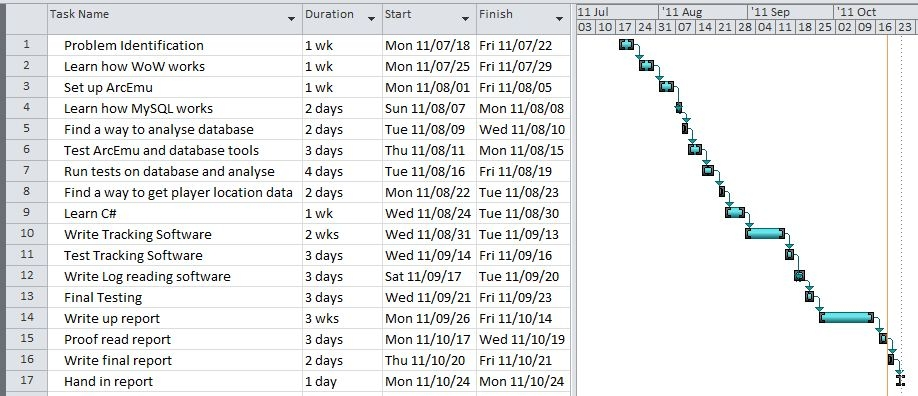
\includegraphics[angle = 90, scale = 0.7]{gantchart.jpg}	
%\end{figure}

\begin{table}[htbp]
  \centering
  \caption{Planning Schedule}
    \begin{tabular}{llrr}
    \addlinespace
    \toprule
    \textbf{Planned schedule} &       &       &  \\
    \midrule
    \textbf{Task Name} & \textbf{Duration} & \textbf{Start} & \textbf{Finish} \\
    \midrule
    Problem Identification & 1 week & 2011/07/18 & 2011/07/24 \\
    Learn how WoW works & 1 week & 2011/07/25 & 2011/07/31 \\
    Set up ArcEmu & 1 week & 2011/08/01 & 2011/08/08 \\
    Find a way to analyse database & 2 days & 2011/08/09 & 2011/08/10 \\
    Run tests on ArcEmu and database & 10 days & 2011/08/11 & 2011/08/21 \\
    Find a way to get player location data & 2 days & 2011/08/22 & 2011/08/23 \\
    Learn C\# & 1 week & 2011/08/24 & 2011/08/30 \\
    Write and test tracking and & 24 days & 2011/08/31 & 2011/09/23 \\
    log reading software &       &       &  \\
    Write Report & 3 weeks & 2011/09/26 & 2011/10/16 \\
    Proof read report & 3 days & 2011/10/17 & 2011/10/19 \\
    Write final report & 2 days & 2011/10/20 & 2011/10/21 \\
    Hand in report & 1 day & 2011/10/24 & 2011/10/24 \\
    \midrule
    \textbf{Actual Schedule} &       &       &  \\
    \midrule
    Problem Identification & 1 week & 2011/07/18 & 2011/07/24 \\
    Learn how WoW works & 4 days & 2011/07/25 & 2011/07/28 \\
    Set up ArcEmu & 1 week & 2011/07/29 & 2011/08/04 \\
    Find a way to analyse database & 2 days & 2011/08/05 & 2011/08/06 \\
    Run tests on ArcEmu and database & 9 days & 2011/08/07 & 2011/08/15 \\
    Find a way to get player location data & 10 days & 2011/08/16 & 2011/08/25 \\
    Learn C\# & 1 week & 2011/08/26 & 2011/09/01 \\
    Write and test tracking and & 3 weeks & 2011/09/02 & 2011/09/23 \\
    log reading software &       &       &  \\
    Write Report & 27 days & 2011/09/24 & 2011/10/20 \\
    Proof read report & 3 days & 2011/10/21 & 2011/10/21 \\
    Write and read final report & 2 days & 2011/10/22 & 2011/10/23 \\
    Hand in report & 1 day & 2011/10/24 & 2011/10/24 \\
    \bottomrule
    \end{tabular}%
\end{table}%

\chapter{Project Specification}

\section{Specifications}
This project had the following specifications:

\begin{enumerate}
	\item Set up a private WoW server for analysing purposes.
	\item Analyse the queries made to the database of the private server.
	\item Write software that can extract and log the movement data of players in WoW on the client side.
	\item Write software that can read logs that are created from the tracking software to display player movement traces.
	\item Test the software to ensure the integrity of the movement data it produces.
\end{enumerate}

\section{Performance}
The performance of the software follows:

\begin{enumerate}
	\item The software reads the memory of the WoW client to extract location data of players.
	\item The software can get and log the location data of players accurately every 10 ms.
	\item The software can draw player traces in real time.
	\item The log reading software can read logs in batch and produce player traces accurately from the logs.
	\item The log reading software can save the traces to a bitmap file of up to 10 000 mega pixels.
\end{enumerate}

%Include the specifications of the project

\chapter{Outcome Compliance}

\begin{table}[htbp]
\centering
\caption{Outcome compliance}
\label{Outcome_compliance}
\begin{tabular}{|l|c|}
  \hline
  \textbf{Outcomes} & \textbf{Chapters} \\
  \hline
  Identification of problems, suggestion and implementation &\\
  of solutions & 1, 3, 4, 5 \\
  \hline
  Application of a knowledge of mathematics and basic &\\
  engineering science in implementing solutions & 3, 4 \\
  \hline
  Implementation of solutions through the design of &\\
  components,subsystems and systems & 3, 4 \\
  \hline
  Gathering information, analysing it critically, and &\\
  then drawing sensible conclusions & 5, 6 \\
  \hline
  Effective use of aids such as measurement equipment and software &\\
  in order to verify and analyse designs & 2, 3, 4 \\
  \hline
  Effective reporting of the project in written form & All \\
  \hline
  Demonstration of the ability of independent learning & All \\
  \hline
  Report writing & All \\
  \hline
\end{tabular}
\end{table}
\chapter{C code listing}
The code for the player tracking software and log reading software is listed in this Appendix in different sections. Each separate file in the programs are listed in their own code blocks.

\section{Player Tracking Software}

\lstset{language=c}
\lstset{basicstyle=\small}
%\lstset{backgroundcolor=listinggray,framerulecolor=blue}
%\lstset{backgroundcolor=listinggray,rulecolor=blue}
\lstset{backgroundcolor=\color{listinggray},rulecolor=\color{blue}}
\lstset{linewidth=\textwidth}
%\lstset{labelstep=10}
%\lstset{commentstyle=\textit, stringstyle=\upshape,stringspaces=false}
\lstset{commentstyle=\textit, stringstyle=\upshape,showspaces=false}
\lstset{frame=trBL,frameround=tttt}


File: WoWdar.cs
\begin{lstlisting}
using System;
using System.Collections.Generic;
using System.Collections;
using System.ComponentModel;
using System.Data;
using System.Drawing;
using System.Linq;
using System.Text;
using System.Windows.Forms;
using Magic;

namespace WoWdar
{
public partial class WoWdar : Form
{
  uint ClientCon = 0;
  uint ObjectMan = 0;
  uint FirstObj = 0;
  uint TotWowObj = 0;
  uint WoWBase = 0;
  bool TrackerReady = false;
  ArrayList allObjects = new ArrayList();
  ArrayList objGuid = new ArrayList();
  bool Found = false;
         
  static int DisplayHeight = 552;
  static int DisplayWidth = 552;
  Bitmap TrackingBitmap = new Bitmap(DisplayWidth, DisplayHeight);
  float TZoom = 1;        //default zoom level
  //dont show units that are 100 higher or lower than yourself
  int absZRange = 100; 
  
  //color definitions
  Color PlayerColor = Color.Blue;
  Color DeadPlayer = Color.DarkBlue;
  Color LiveNPC = Color.Plum;
  Color DeadNPC = Color.Gray;
  Color LocalPlayer = Color.ForestGreen;
  Color CurrentTarget = Color.Red;

  WoWObject Player = new WoWObject();
  WoWObject Me = new WoWObject();
  WoWObject Target = new WoWObject();
  WoWObject CurrentObj = new WoWObject();
  WoWObject TempObj = new WoWObject();
  BlackMagic wow = new BlackMagic();

  public WoWdar()
  {
    InitializeComponent();
  }


  private void WoWdar_Load(object sender, EventArgs e)
  {
   try
   {
     if (LoadOffsets() == true)
        TrackerReady = true;

     if (TrackerReady == false)
     {
        ClearBitmap(ref TrackingBitmap);
        TrackingBitmap = WriteTextCenter(TrackingBitmap, 
          "Please enter the game world and click Reload.", 8);
        display.Image = TrackingBitmap;
     }
    }
    catch(Exception)
    {
      ClearBitmap(ref TrackingBitmap);
      TrackingBitmap = WriteTextCenter(TrackingBitmap, 
        "Could not load offsets. Please Reload.", 8);
      display.Image = TrackingBitmap;
    }        
   }

  private Boolean LoadOffsets()
  {
    if (wow.OpenProcessAndThread(
      SProcess.GetProcessFromProcessName("Wow")))
    {
    }
    else
    {
      return false;
    }

    IntPtr baseWoW = wow.MainModule.BaseAddress;
    WoWBase = (uint)baseWoW;

    ClientCon = wow.ReadUInt((uint)baseWoW 
      + (uint)ObjectManagerOff.clientConnection);
    ObjectMan = wow.ReadUInt(ClientCon 
      + (uint)ObjectManagerOff.objectManager);
    FirstObj = wow.ReadUInt(ObjectMan 
      + (uint)ObjectManagerOff.firstObject);
    Target.GUID = wow.ReadUInt64((uint)baseWoW 
      + (uint)PlayerOff.LastTargetGUID);
    Me.GUID = wow.ReadUInt64(ObjectMan 
      + (uint)ObjectManagerOff.localGuid);
    Me.Name = wow.ReadASCIIString((uint)baseWoW + 0x980598, 20);
            
    this.pName.Text = "Name: " + Me.Name;
    this.pGuid.Text = "GUID: " + Me.GUID;

    if (Me.GUID == 0)
      return false;
    else
      return true;

  }

  private float RadToDeg(float Rot)
  {
    return (float)(Rot * (180 / Math.PI));
  }

  private void RadarTimer_Tick(object sender, EventArgs e)
  {
    if(rZoom1.Checked)
    {
                TZoom = 1;
    }
    else if(rZoom2.Checked)
    {
      TZoom = 2;
    }
    else if (rZoom3.Checked)
    {
      TZoom = 3;
    }
    else if (rZoom4.Checked)
    {
       TZoom = 4;
    }
 
    //don't clear bitmap if traces must be shown
    if(!cbShowTrace.Checked) 
    {
       ClearBitmap(ref TrackingBitmap);
    }

    if (TrackerReady == false)
    {
      TrackingBitmap = WriteTextCenter(TrackingBitmap, 
        "Please enter the game world then click Reload.", 8);
      display.Image = TrackingBitmap;
      return;
    }

    try
    {
      TotWowObj = 0;
      CurrentObj.BaseAddress = FirstObj;
      Target.GUID = wow.ReadUInt64(WoWBase 
        + (uint)PlayerOff.LastTargetGUID);

      Me.BaseAddress = GetBaseByGuid(Me.GUID);
      Me.X = wow.ReadFloat(Me.BaseAddress 
        + (uint)ObjectOffsets.Pos_X);
      Me.Y = wow.ReadFloat(Me.BaseAddress 
        + (uint)ObjectOffsets.Pos_Y);
      Me.Z = wow.ReadFloat(Me.BaseAddress 
        + (uint)ObjectOffsets.Pos_Z);
      Me.Rot = wow.ReadFloat(Me.BaseAddress 
        + (uint)ObjectOffsets.Rot);

      Graphics g = Graphics.FromImage(TrackingBitmap);

      if (Target.GUID != 0)    //if valid target, get target details
      {
        Target.BaseAddress = GetBaseByGuid(Target.GUID);
        Target.X = wow.ReadFloat(Target.BaseAddress 
          + (uint)ObjectOffsets.Pos_X);
        Target.Y = wow.ReadFloat(Target.BaseAddress 
          + (uint)ObjectOffsets.Pos_Y);
        Target.Z = wow.ReadFloat(Target.BaseAddress 
          + (uint)ObjectOffsets.Pos_Z);
        Target.Rot = wow.ReadFloat(Target.BaseAddress 
          + (uint)ObjectOffsets.Rot);
        Target.ObjectFields = wow.ReadUInt(Target.BaseAddress 
          + (uint)ObjectOffsets.ObjectFields);
        Target.Type = wow.ReadShort(Target.BaseAddress + 0x14);

        if (Target.Type == 3)    //NPC 
        {
           Target.Name = NPCNameFromGuid(Target.GUID);
        }
        if (Target.Type == 4)    //human player
        {
           Target.Name = PlayerNameFromGuid(Target.GUID);
        }
        if ((Target.Type != 4) && (Target.Type != 3))
        {
          Target.Name = "Object.";
        }

     }//end if Target Guid !=0

//now go through all objects and add new ones to array list 
//and update old ones (all for logging purposes).
//also display all objects

     while ((CurrentObj.BaseAddress != 0) 
        && (CurrentObj.BaseAddress % 2 == 0))
     {
       TotWowObj += 1;     //count all wow objects in range

       CurrentObj.GUID = GetGuidByBase(CurrentObj.BaseAddress);
       CurrentObj.ObjectFields = wow.ReadUInt(CurrentObj.BaseAddress 
         + (uint)ObjectOffsets.ObjectFields);
       CurrentObj.Type = wow.ReadShort(CurrentObj.BaseAddress 
         + 0x14);
       CurrentObj.X = wow.ReadFloat(CurrentObj.BaseAddress 
         + (uint)ObjectOffsets.Pos_X);
       CurrentObj.Y = wow.ReadFloat(CurrentObj.BaseAddress 
         + (uint)ObjectOffsets.Pos_Y);
       CurrentObj.Z = wow.ReadFloat(CurrentObj.BaseAddress 
         + (uint)ObjectOffsets.Pos_Z);
       CurrentObj.Rot = wow.ReadFloat(CurrentObj.BaseAddress 
         + (uint)ObjectOffsets.Rot);
       CurrentObj.health = wow.ReadUInt(CurrentObj.ObjectFields 
         + (uint)UnitFields.UNIT_FIELD_HEALTH);

       if (CurrentObj.Type == 3)    //NPC 
       {
         CurrentObj.Name = NPCNameFromGuid(CurrentObj.GUID);
       }
       if (CurrentObj.Type == 4)    //human player
       {
         CurrentObj.Name = PlayerNameFromGuid(CurrentObj.GUID);
       }

//is target is within reasonable vertical range & not me ? 

       if ((Math.Abs(Me.Z - CurrentObj.Z) <= absZRange) 
         && (CurrentObj.GUID != Me.GUID))         
       {                                                                                                                          
         switch (CurrentObj.Type)
         {
           case 3: //npc
          //only draw NPC if showtrace not checked
             if (!cbShowTrace.Checked)   
             {
               if (CurrentObj.health <= 0)
               {
                 TrackingBitmap = SketchPlayer(TrackingBitmap, 
                   DeadNPC, (Me.X - CurrentObj.X) * TZoom 
                   + DisplayWidth / 2, (Me.Y - CurrentObj.Y) 
                   * TZoom + DisplayHeight / 2, CurrentObj.Rot, 
                   CurrentObj.Name);
               }//NPC dead
               else
               {
                 TrackingBitmap = SketchPlayer(TrackingBitmap, 
                   LiveNPC, (Me.X - CurrentObj.X) * TZoom 
                   + DisplayWidth / 2, (Me.Y - CurrentObj.Y) 
                   * TZoom + DisplayHeight / 2, CurrentObj.Rot, 
                   CurrentObj.Name);
               }//NPC alive
             }                                
             break;

          case 4: //a player

             if(CurrentObj.health <= 0)
             {
               TrackingBitmap = SketchPlayer(TrackingBitmap, 
                 DeadPlayer, (Me.X - CurrentObj.X) * TZoom 
                 + DisplayWidth / 2, (Me.Y - CurrentObj.Y) 
                 * TZoom + DisplayHeight / 2, CurrentObj.Rot, 
                 CurrentObj.Name);
             }//player dead
             else
             {       //track living human players
               if(cbTrack.Checked)
               {
                 if (allObjects.Count <= 0) //first entry in array
                 {
                   TimeAndPos temp = new TimeAndPos();
                   temp.XPos = CurrentObj.X;
                   temp.YPos = CurrentObj.Y;
                   temp.ZPos = CurrentObj.Z;
                   temp.RotPos = CurrentObj.Rot;
                   temp.time = DateTime.Now;       
                   ObjArray trackPlayer = new ObjArray();
                   trackPlayer.GUID = CurrentObj.GUID;
                   trackPlayer.info.Add(temp);
                   allObjects.Add(trackPlayer);
                 }
//search through array to see if player is already there                
                 else                    
                 {
                   foreach(ObjArray tracking in allObjects)
                   {
                   //means current player GUID already in array
                     if (tracking.GUID == CurrentObj.GUID)
                     {
                       Found = true;
                       TimeAndPos temp = new TimeAndPos();
                       temp.XPos = CurrentObj.X;
                       temp.YPos = CurrentObj.Y;
                       temp.ZPos = CurrentObj.Z;
                       temp.RotPos = CurrentObj.Rot;
                       temp.time = DateTime.Now;
                       tracking.info.Add(temp);
                     }
                   }
                   //item not found in list, add it to list
                   if (!Found)     
                   {
                     TimeAndPos temp = new TimeAndPos();
                     temp.XPos = CurrentObj.X;
                     temp.YPos = CurrentObj.Y;
                     temp.ZPos = CurrentObj.Z;
                     temp.RotPos = CurrentObj.Rot;
                     temp.time = DateTime.Now;      
                     ObjArray trackPlayer = new ObjArray();
                     trackPlayer.GUID = CurrentObj.GUID;
                     trackPlayer.info.Add(temp);
                     allObjects.Add(trackPlayer);
                   }
                   else
                   {
                     Found = false;  //reset value
                   }
                   lTest.Text = "Total Players: " + allObjects.Count;
                }
              }
              TrackingBitmap = SketchPlayer(TrackingBitmap, 
                PlayerColor, (Me.X - CurrentObj.X) * TZoom 
                + DisplayWidth / 2, (Me.Y - CurrentObj.Y) 
                * TZoom + DisplayHeight / 2, CurrentObj.Rot, 
                CurrentObj.Name);
           }//Player alive
           break;
         }//end switch
        }//end if
        CurrentObj.BaseAddress = wow.ReadUInt(CurrentObj.BaseAddress 
          + (uint)ObjectManagerOff.nextObject);
      }//end while loop of all objects

      this.pName.Text = "Name: " + Me.Name;
      this.pGuid.Text = "GUID: " + Me.GUID;
      this.pX.Text = "X: " + Me.X.ToString();
      this.pY.Text = "Y: " + Me.Y;
      this.pZ.Text = "Z: " + Me.Z;
      this.pRotRad.Text = "Rotation in Rad: " 
        + Math.Round(Me.Rot, 2).ToString() + " R";
      this.pRotDeg.Text = "Rotation in Deg: " 
        + Math.Round(RadToDeg(Me.Rot), 2).ToString() + " D";
      TrackingBitmap = SketchPlayer(TrackingBitmap, 
         LocalPlayer, (Me.X - Me.X) * TZoom 
         + DisplayWidth / 2, (Me.Y - Me.Y) * TZoom 
         + DisplayHeight / 2, Me.Rot, Me.Name);

      if (Target.GUID != 0)
      {
        this.tName.Text = "Name: " + Target.Name;
        this.tGuid.Text = "GUID: " + Target.GUID;
        this.tX.Text = "X: " + Target.X.ToString();
        this.tY.Text = "Y: " + Target.Y;
        this.tZ.Text = "Z: " + Target.Z;
        this.tRotRad.Text = "Rotation in Rad: " 
          + Math.Round(Target.Rot, 2).ToString() + " R";
        this.tRotDeg.Text = "Rotation in Deg: " 
          + Math.Round(RadToDeg(Target.Rot), 2).ToString() + " D";
        TrackingBitmap = SketchPlayer(TrackingBitmap, 
           CurrentTarget, (Me.X - Target.X) * TZoom 
           + DisplayWidth / 2, (Me.Y - Target.Y) * TZoom 
           + DisplayHeight / 2, Target.Rot, Target.Name);
      }//end if
      else
      {
        this.tName.Text = "Name: ";
        this.tGuid.Text = "GUID: 0";
        this.tX.Text = "X: ";
        this.tY.Text = "Y: ";
        this.tZ.Text = "Z: ";
        this.tRotRad.Text = "Rotation in Rad: ";
        this.tRotDeg.Text = "Rotation in Deg: ";
      }//end else
    
      display.Image = TrackingBitmap;
      lTotObj.Text = "Total Objects: " + TotWowObj;
    }
    catch(Exception)
    {
      return;
    }
  }

  public string NPCNameFromGuid(ulong Guid)
  {
    uint ObjectBase = GetBaseByGuid(Guid);
    if(ObjectBase == 0)
    {
      return "Name not found";
    }
    try
    {
      return wow.ReadASCIIString(wow.ReadUInt(
         wow.ReadUInt(ObjectBase + (uint)NameOffsets.UnitName1)
         + (uint)NameOffsets.UnitName2), 30);
    }
    catch(Exception)
    {
      return "Exception";
    }
  }//end MobNameFromGuid

  public uint GetBaseByGuid(ulong Guid)
  {
    TempObj.BaseAddress = FirstObj;     //start from first object
//loop through all objects till right one is found
    while (TempObj.BaseAddress != 0)    
    {
      try
      {
        TempObj.GUID = wow.ReadUInt64(TempObj.BaseAddress 
          + (uint)ObjectOffsets.Guid);
      }
      catch(Exception)
      {
        TempObj.GUID = 0;
      }
      if(TempObj.GUID == Guid)
      {
        return TempObj.BaseAddress;
      }
      try
      {
        TempObj.BaseAddress = wow.ReadUInt(TempObj.BaseAddress 
          + (uint)ObjectManagerOff.nextObject);    
          //move on to next object
      }
      catch (Exception)
      {
        return 0;
      }
    }
   return 0;   //return 0 if nothing is found.
  }//end GetObjectBaseByGuid


// Credits WhatSupMang, SillyBoy72 of OwnedCore.com
  public string PlayerNameFromGuid(ulong Guid)
  {
    ulong mask, base_, offset, current, shortGUID, testGUID;
    try
    {
      mask = wow.ReadUInt(WoWBase + (uint)NameOffsets.nameStore 
        + (uint)NameOffsets.nameMask);
    }
    catch (Exception)
    {
      return "Exception";
    }

    base_ = wow.ReadUInt(WoWBase + (uint)NameOffsets.nameStore 
      + (uint)NameOffsets.nameBase);

    shortGUID = Guid & 0xffffffff;
    offset = 12 * (mask & shortGUID);
    try
    {
      current = wow.ReadUInt((uint)base_ + (uint)offset + 8);
    }
    catch (Exception)
    {
      return "Exception";
    }

    offset = wow.ReadUInt((uint)base_ + (uint)offset);

    if ((current & 0x1) == 0x1) { return ""; }

    try
    {
      testGUID = wow.ReadUInt((uint)current);
    }
    catch (Exception)
    {
      return "Exception";
    }

    while (testGUID != shortGUID)
    {
      current = wow.ReadUInt((uint)current + (uint)offset + 4);
      
      if ((current & 0x1) == 0x1) { return ""; }
      try
      {
        testGUID = wow.ReadUInt((uint)current);
      }
      catch (Exception)
      {
        return "Exception";
      }
    }
   return wow.ReadASCIIString((uint)current 
     + (uint)NameOffsets.nameString, 30);
  }//end PlayerNameFromGuid

  private ulong GetGuidByBase(uint Base)
  {
    return wow.ReadUInt64(Base + (uint)ObjectOffsets.Guid);
  }//end GetObjectGuidByBase


// the rest of the methods are all for drawing the objects

  private Bitmap SketchPlayer(Bitmap img, 
     Color UnitColor, float Ypos, 
     float Xpos, float Rotation, string strName)
  {
    Graphics G = Graphics.FromImage(img);

    G.SmoothingMode = System.Drawing.
       Drawing2D.SmoothingMode.HighQuality;

    Pen NormalPen = new Pen(UnitColor, 2F);
    Pen TracingPen = new Pen(UnitColor, 0.1F); //for showing traces

    Rotation = RadToDeg(Rotation);

    G.ResetTransform();     //Resets the transformation matrix
    G.TranslateTransform(-Xpos, -Ypos, 
    System.Drawing.Drawing2D.MatrixOrder.Append);        
    //move drawing coordinates to origin
    try
    {
      G.RotateTransform(-Rotation, 
        System.Drawing.Drawing2D.MatrixOrder.Append);          
      //rotate counterclockwise at origin
    }
    catch (ArgumentException)
    {
    }
    G.TranslateTransform(Xpos, Ypos,
      System.Drawing.Drawing2D.MatrixOrder.Append);           
    //move back to drawing coordinates
    try
    {
      if (!cbShowTrace.Checked)    //how to draw when not tracing
      {
        G.DrawLine(NormalPen, Xpos - 2, Ypos + 2, Xpos, Ypos - 6);
        G.DrawLine(NormalPen, Xpos + 2, Ypos + 2, Xpos, Ypos - 6);
        G.DrawLine(NormalPen, Xpos, Ypos - 2, Xpos, Ypos - 6);
        G.DrawLine(NormalPen, Xpos - 2, Ypos +1, Xpos + 2, Ypos +1);

        if(!cbNames.Checked)
        {
          WriteText(img, strName, Convert.ToInt32(Xpos) 
            - Convert.ToInt32((strName.Length) * 2.5), 
            Convert.ToInt32(Ypos) + 6);
        }

      }
      else//when tracing
      {
        G.DrawLine(TracingPen, Xpos, Ypos, Xpos, Ypos - 3);
      }
    }
    catch (Exception ex)
    {
    }
    G.Dispose();
    NormalPen.Dispose();
    TracingPen.Dispose();
    return img;
  }//end sketchplayer 

  private Bitmap WriteText(Bitmap img, 
    String sText, int XPos, int YPos)
  {
    Graphics G = Graphics.FromImage(img);
    G.SmoothingMode = System.Drawing.
      Drawing2D.SmoothingMode.HighQuality;
    Font DrawFont = new Font("Arial", 7);
    G.DrawString(sText, DrawFont, 
      Brushes.Black, new Point(XPos, YPos));
    G.Dispose();
    DrawFont.Dispose();
    return img;
  }

  private Bitmap WriteTextCenter(Bitmap img, String sText, int size)  
  // will draw on center of image
  {
    Graphics G = Graphics.FromImage(img);
    G.SmoothingMode = System.Drawing.
      Drawing2D.SmoothingMode.HighQuality;
    Font TextFont = new Font("Arial", size);
    StringFormat SF = new StringFormat();
    SF.LineAlignment = StringAlignment.Center;
    SF.Alignment = StringAlignment.Center;
    RectangleF Rect = new RectangleF(0, 0, 
      DisplayWidth, DisplayHeight);
    G.DrawString(sText, TextFont, Brushes.Black, Rect, SF);
    G.Dispose();
    TextFont.Dispose();
    SF.Dispose();
    return img;
  }

  private void ClearBitmap(ref Bitmap img)
  {
    Graphics G = Graphics.FromImage(img);
    G.Clear(display.BackColor);
    G.Dispose();
  }

  private void bReload_Click(object sender, EventArgs e)
  {
    try
    {
      if (LoadOffsets() == true)
        TrackerReady = true;

      if (TrackerReady == false)
      {
        ClearBitmap(ref TrackingBitmap);
        TrackingBitmap = WriteTextCenter(TrackingBitmap, 
          "Please enter the game world.", 8);
        display.Image = TrackingBitmap;
      }
    }
    catch (Exception)
    {
      ClearBitmap(ref TrackingBitmap);
      TrackingBitmap = WriteTextCenter(TrackingBitmap, 
        "Could not load offsets. Please Reload.", 8);
      display.Image = TrackingBitmap;
    }  
  }

  private void cbOnTop_CheckedChanged(object sender, EventArgs e)
  {
    if (cbOnTop.Checked)
    {
       WoWdar.ActiveForm.TopMost = true;
    }
    else
    {
       WoWdar.ActiveForm.TopMost = false;
    }
  }

  private void bLog_Click(object sender, EventArgs e)
  {
    Log saveLog = new Log();
    saveLog.WriteToFile(allObjects);
    allObjects.Clear();
  }

  private void cbShowTrace_CheckedChanged(object sender, EventArgs e)
  {
    ClearBitmap(ref TrackingBitmap);
  }

  private void cbNames_CheckedChanged(object sender, EventArgs e)
  {
    ClearBitmap(ref TrackingBitmap);
  }
 }
}

\end{lstlisting}

File: Logs.cs
\begin{lstlisting}
using System;
using System.IO;
using System.Collections.Generic;
using System.Collections;
using System.Linq;
using System.Text;

namespace WoWdar
{
  class Log
  {

    public void WriteToFile(ArrayList datalist)
    {
      foreach(ObjArray obj in datalist)
      {
        using (StreamWriter w = File.AppendText(obj.GUID + ".txt"))
        {
          foreach(TimeAndPos data in obj.info)
          {
            w.WriteLine(data.time.ToString("yyyy/MM/dd,HH:mm:ss.fff") 
            + "," + data.XPos + "," + data.YPos + ","+ data.ZPos 
            + "," + data.RotPos);     //write data to log file
          }
          w.Flush();  //write and clear all buffered text
          w.Close();  //close file
        }
      }
    }
  }
}

\end{lstlisting}

File: Struct.cs
\begin{lstlisting}

using System;
using System.Collections.Generic;
using System.Collections;
using System.Linq;
using System.Text;

namespace WoWdar
{
  //this struct is for logging location information purposes.
  public struct TimeAndPos
  {
    public DateTime time;
    public float XPos;
    public float YPos;
    public float ZPos;
    public float RotPos;
  }//end struct
}

\end{lstlisting}


File: ObjArray.cs
\begin{lstlisting}
using System;
using System.Collections.Generic;
using System.Collections;
using System.Linq;
using System.Text;

namespace WoWdar
{
//this class is for logging location information purposes.
    class ObjArray
    {
        public ulong GUID = 0;
        public ArrayList info = new ArrayList();
    }
}

\end{lstlisting}

File: Offsets.cs
\begin{lstlisting}
using System;
using System.Collections.Generic;
using System.Linq;
using System.Text;

namespace WoWdar
{
//offsets for WoW 4.2.2.14545

  public enum ObjectManagerOff : uint
  {
    clientConnection = 0x980558,
    objectManager = 0x463C,
    firstObject = 0xB4,
    nextObject = 0x3C,
    localGuid = 0xB8
  }

  public enum PlayerOff : uint
  {
    LastTargetGUID = 0x00A98C80,   //0xA98C88,
    playerName = 0x980598,
  }

  public enum GameObject
  {
    objName1 = 0x1CC,
    objName2 = 0xB4,
  }

  public enum ObjectFields : uint
  {
    OBJECT_FIELD_GUID = 0x0,
    OBJECT_FIELD_DATA = 0x8,
    OBJECT_FIELD_TYPE = 0x10,
  }

  public enum NameOffsets : ulong
  {
    ObjectName1 = 0x1CC,
    ObjectName2 = 0xB4,
    UnitName1 = 0x91C,  //0x142?
    UnitName2 = 0x64,   //0x15E?
    nameStore = 0x959EE0 + 0x8,
    nameMask = 0x24,
    nameBase = 0x1C,
    nameString = 0x20
  }

  public enum ObjectOffsets : uint
  {
    Pos_X = 0x790,
    Pos_Y = Pos_X + 0x4,
    Pos_Z = Pos_X + 0x8,
    Rot = Pos_X + 0x10,
    Guid = 0x30,
    ObjectFields = 0x8,
  }

  public enum UnitFields
  {
     UNIT_FIELD_HEALTH = 0x68,    
  }
}



\end{lstlisting}

File: Program.cs
\begin{lstlisting}

using System;
using System.Collections.Generic;
using System.Linq;
using System.Windows.Forms;
using Magic;

namespace WoWdar
{
  static class Program
  {
    [STAThread]
    static void Main()
    {
      Application.EnableVisualStyles();
      Application.SetCompatibleTextRenderingDefault(false);
      Application.Run(new WoWdar());
    }
  }
}

\end{lstlisting}

\newpage

\section{Log Reading Program}

File: WoWTraces.cs
\begin{lstlisting}

using System;
using System.IO;
using System.Collections.Generic;
using System.ComponentModel;
using System.Data;
using System.Drawing;
using System.Linq;
using System.Text;
using System.Windows.Forms;

namespace WindowsFormsApplication1
{
public partial class WowTraces : Form
{
  string ChosenFile = "";
  string path = Environment.CurrentDirectory;
  bool first = true;
  char[] delimiter = {','};
  float Xref = 0;
  float Yref = 0;
  float X = 0;
  float fZoom = 1;
  float Y = 0;
  static int size = 917;
  float Rot = 0;
  Bitmap TraceBitmap = new Bitmap(size, size);
  Bitmap SaveBitmap;

  public WowTraces()
  {
    InitializeComponent();
  }

  private void mnuLoad_Click(object sender, EventArgs e)
  {
    openFD.FileName = "";
    openFD.Title = "Select log file.";
    openFD.InitialDirectory = path;
    openFD.Filter = "LOG FILE|*.txt";

    if (openFD.ShowDialog() != DialogResult.Cancel)
    {
      ChosenFile = openFD.FileName;
    }
    else
    {
      ChosenFile = "";
    }
  }

  private void button1_Click(object sender, EventArgs e)
  {
    SaveBitmap = new Bitmap(int.Parse(nWidth.Value.ToString()), 
      int.Parse(nHeigth.Value.ToString()));
    Graphics G = Graphics.FromImage(SaveBitmap);
    G.Clear(iTraces.BackColor);
    G.Dispose();

    if (ChosenFile == "")//make sure a file is chosen
    {
      MessageBox.Show("Please select a file first.");
    }
    else
    {
      //sets the zoom level according to option chosen
      if(rbZoom1.Checked)
      {
        fZoom = 1;
      }
    else if (rbZoom2.Checked)
    {
      fZoom = 2;
    }
    else if (rbZoom3.Checked)
    {
      fZoom = 3;
    }
    else if (rbZoom4.Checked)
    {
      fZoom = 4;
    }
    else if (rbZoom05.Checked)
    {
      fZoom = 0.5F;
    }
    else if (rbZoom5.Checked)
    {
      fZoom = 5;
    }

    try
    {
      using (StreamReader sr = new StreamReader(ChosenFile))
      {
        String line;
        while ((line = sr.ReadLine()) != null)
        {
          string[] info = line.Split(delimiter);
          if (info.Length == 6)
          {
            if (first)
            {
              first = false;
              Xref = float.Parse(info[2]);
              Yref = float.Parse(info[3]);
              lXref.Text = "Xref :" + Xref;
              lYref.Text = "Yref :" + Yref;
            }
            X = float.Parse(info[2]);
            Y = float.Parse(info[3]);
            Rot = float.Parse(info[5]);

            TraceBitmap = SketchPlayer(TraceBitmap, Color.Blue, 
              (Xref - X)*fZoom + iTraces.Width / 2, (Yref - Y)
              *fZoom + iTraces.Height / 2, Rot);
            SaveBitmap = SketchPlayer(SaveBitmap, Color.Blue, 
              (Xref - X) * fZoom + SaveBitmap.Width / 2, (Yref - Y) 
              * fZoom + SaveBitmap.Height / 2, Rot);
          }
          else
          {
          }
        }
      }
    }
    catch (Exception ex)
    {
      MessageBox.Show("File could not be read.");
    }
    iTraces.Image = TraceBitmap;
   }
  }

  private void bAllTraces_Click(object sender, EventArgs e)
  {
    string path = Environment.CurrentDirectory;
    DirectoryInfo dir = new DirectoryInfo(path);
    SaveBitmap = new Bitmap(int.Parse(nWidth.Value.ToString()), 
      int.Parse(nHeigth.Value.ToString()));
    Graphics G = Graphics.FromImage(SaveBitmap);
    G.Clear(iTraces.BackColor);
    G.Dispose();
            
//sets the zoom level according to option chosen
    if (rbZoom1.Checked)
    {
      fZoom = 1;
    }
    else if (rbZoom2.Checked)
    {
      fZoom = 2;
    }
    else if (rbZoom3.Checked)
    {
      fZoom = 3;
    }
    else if (rbZoom4.Checked)
    {
      fZoom = 4;
    }
    else if (rbZoom05.Checked)
    {
      fZoom = 0.5F;
    }
    else if (rbZoom5.Checked)
    {
      fZoom = 5;
    }

    foreach (FileInfo f in dir.GetFiles("*.txt"))
    {
      try
      {
        String name = f.Name;

        using (StreamReader sr = new StreamReader(name))
        {
          String line;
          while ((line = sr.ReadLine()) != null)
          {
            string[] info = line.Split(delimiter);  
            //small test to ensure right format of log
            if (info.Length == 6)
            {
              if(first)
              {
                first = false;
                Xref = float.Parse(info[2]);
                Yref = float.Parse(info[3]);
                lXref.Text = "Xref :" + Xref;
                lYref.Text = "Yref :" + Yref;
              }
              X = float.Parse(info[2]);
              Y = float.Parse(info[3]);
              Rot = float.Parse(info[5]);

              TraceBitmap = SketchPlayer(TraceBitmap, 
                Color.Blue, (Xref - X)*fZoom + iTraces.Width/2, 
                (Yref - Y)*fZoom + iTraces.Height/2, Rot);
              SaveBitmap = SketchPlayer(SaveBitmap, 
                Color.Blue, (Xref - X)*fZoom + SaveBitmap.Width/2, 
                (Yref - Y) * fZoom + SaveBitmap.Height / 2, Rot);
            }
            else
            {
            }
          }
        }
      }
      catch (Exception ex)
      {
        MessageBox.Show("File could not be read.");
      }
    }
    iTraces.Image = TraceBitmap;
  }

  private void bClear_Click(object sender, EventArgs e)
  {
    first = true;
    Xref = 0;
    Yref = 0;
    Graphics G = Graphics.FromImage(TraceBitmap);
    G.Clear(iTraces.BackColor);
    G.Dispose();

    Graphics G1 = Graphics.FromImage(SaveBitmap);
    G1.Clear(iTraces.BackColor);
    G1.Dispose();

    iTraces.Image = TraceBitmap;
  }

  private float RadToDeg(float Rot)
  {
    return (float)(Rot * (180 / Math.PI));
  }

  private Bitmap SketchPlayer(Bitmap img, Color UnitColor, 
    float Ypos, float Xpos, float Rotation)
  {
    Graphics G = Graphics.FromImage(img);
    G.SmoothingMode = System.Drawing.
      Drawing2D.SmoothingMode.HighQuality;
    Pen TracePen = new Pen(UnitColor, 1F);

    Rotation = RadToDeg(Rotation);
    G.ResetTransform();     //Resets the matrix
    G.TranslateTransform(-Xpos, -Ypos, 
      System.Drawing.Drawing2D.MatrixOrder.Append);        
      //move drawing coordinates to origin
    try
    {
      G.RotateTransform(-Rotation, 
        System.Drawing.Drawing2D.MatrixOrder.Append);          
        //rotate counterclockwise at origin
    }
    catch (ArgumentException)
    {
    }
    G.TranslateTransform(Xpos, Ypos, 
      System.Drawing.Drawing2D.MatrixOrder.Append);          
      //move back to drawing coordinates
    try
    {
      if(rbArrow.Checked)
      {
        G.DrawLine(TracePen, Xpos - 2, Ypos + 1, Xpos, Ypos - 3);
        G.DrawLine(TracePen, Xpos + 2, Ypos + 1, Xpos, Ypos - 3);
        G.DrawLine(TracePen, Xpos, Ypos, Xpos, Ypos - 3);
      }
      else if(rbLine.Checked)
      {
        G.DrawLine(TracePen, Xpos, Ypos, Xpos, Ypos - 3);
      }
    }
    catch (Exception ex)
    {
    }
    G.Dispose();
    TracePen.Dispose();
    return img;
  }

  private void btnSave_Click(object sender, EventArgs e)
  {
    SaveBitmap.Save("traces.bmp", 
      System.Drawing.Imaging.ImageFormat.Bmp);
  }
}
}


\end{lstlisting}
%\chapter{MATLAB code listing}

\end{document}


%onthou daai character achievement ding en hoe baie dit groei! noem dit in results!